\documentclass[
  % anonymous,
  % print,
]{shtthesis}

\shtsetup{
  degree = {master},
  degree-name = {工学硕士},
  degree-name* = {Master~of~Science~in~Engineering},
  title = {量化神经网络的训练方法及其在目标检测中的应用},
  title* = {Training~Quantized~Neural~Networks\\and\\Its~Application~in~Object~Detection},
  keywords = {高效深度学习,量化神经网络,目标检测},
  keywords* = {Efficient~Deep~Learning, Quantized~Neural~Networks, Object~Detection},
  author = {李润东},
  author* = {Li~Rundong},
  institution = {上海科技大学信息科学与技术学院},
  institution* = {School~of~Information~Science~and~Technology\\ShanghaiTech~University},
  supervisor = {范睿~副教授},
  supervisor* = {Professor~Fan~Rui},
  supervisor-institution = {上海科技大学信息科学与技术学院},
  discipline-level-1 = {计算机科学与技术},
  discipline-level-1* = {Computer~Science~and~Technology},
  date = {2020~年~6~月},
  date* = {June,~2020},
}
% ==============================================================================
%  Utility Macros
% ==============================================================================
% ------------------------------------------------------------------------------
%    TODO notes
% ------------------------------------------------------------------------------
\usepackage{xargs}
\usepackage[
  colorinlistoftodos,
  prependcaption,
  textsize = tiny,
  textwidth = 2.6cm,
]{todonotes}
\setlength{\marginparwidth}{2.6cm}
\newcommandx{\unsure}[2][1=]{\todo[linecolor=red,backgroundcolor=red!25,bordercolor=red,#1]{#2}}
\newcommandx{\change}[2][1=]{\todo[linecolor=blue,backgroundcolor=blue!25,bordercolor=blue,#1]{#2}}
\newcommandx{\info}[2][1=]{\todo[linecolor=OliveGreen,backgroundcolor=OliveGreen!25,bordercolor=OliveGreen,#1]{#2}}
\newcommandx{\improvement}[2][1=]{\todo[linecolor=Plum,backgroundcolor=Plum!25,bordercolor=Plum,#1]{#2}}
\newcommandx{\thiswillnotshow}[2][1=]{\todo[disable,#1]{#2}}
% ------------------------------------------------------------------------------
%    Machine learning related stuff
% ------------------------------------------------------------------------------
\usepackage{slashed}
\usepackage{esdiff}
\providecommand{\CE}[2]{\mathrm{CE}\left( #1 \| #2 \right)}
\providecommand{\KL}[2]{D_{\mathrm{KL}}\left( #1 \| #2 \right)}
\providecommand{\Round}[1]{\left\lfloor #1 \right\rceil}
\providecommand{\NoDiff}[1]{\slashed{\nabla} #1}
\providecommand{\FpNet}{f_{\mathcal{W}}}
\providecommand{\QuantNet}{\hat{f}_{\mathcal{W, Q}}}
\providecommand{\NormalDist}[1]{\mathcal{N} \left( #1 \right)}
\providecommand{\EMA}[1]{{ #1 }_{\mathrm{EMA}}}
\providecommand{\Batch}[1]{{ #1 }_{\mathrm{b}}}
\providecommand{\Fold}[1]{{ #1 }_{\mathrm{fold}}}
\providecommand{\Clamp}[1]{\mathrm{clamp}\left( #1 \right)}
\DeclareMathOperator{\sign}{sign}
\providecommand{\mAP}[1]{\mathrm{mAP}^{\mathrm{ #1 }}}
\providecommand{\mAR}[1]{\mathrm{mAR}^{\mathrm{ #1 }}}
\providecommand{\QP}{\texttt{QuantPack}}
% ------------------------------------------------------------------------------
%    Drawing and table helpers
% ------------------------------------------------------------------------------
\usepackage{tikz}
\usetikzlibrary{
  positioning,
  arrows,
  calc,
  trees,
  shapes.geometric,
}
\providecommand\boxit[1]{%
  \smash{\color{red}\fboxrule=1pt\relax\fboxsep=2pt\relax%
  \llap{\rlap{\fbox{\vphantom{0}\makebox[#1]{}}}~}}\ignorespaces%
}
\usepackage{forest}
\usepackage{circledsteps}
% ------------------------------------------------------------------------------
%    Enhanced table, floats and code environments
% ------------------------------------------------------------------------------
\usepackage{ctable}
\usepackage{subcaption}
\usepackage{multirow}
\usepackage{arydshln}
\usepackage{minted}
\usepackage{mdframed}
\definecolor{ShtRed}{RGB}{146, 46, 23}
\definecolor{FriendlyBG}{RGB}{240, 240, 240}
\setminted{
  fontsize=\small,
  style=friendly,
  breaklines,
  breakbytoken,
}
\mdfsetup{
  backgroundcolor=FriendlyBG,
  linecolor=ShtRed,
  linewidth=1pt,
  topline=false,
  bottomline=false,
  rightline=false,
  innertopmargin=2pt,
  innerbottommargin=2pt,
}
\newminted[python]{Python3}{}
\newminted[yaml]{YAML}{}
\BeforeBeginEnvironment{minted}{%
  \begin{mdframed}%
  \linespread{1.3}%
}
\AfterEndEnvironment{minted}{\end{mdframed}}
\captionsetup{subrefformat=parens, font={small,bf}}
\captionsetup[sub]{font={small,bf}}

\begin{document}
\maketitle
\frontmatter
% ~~~~~~~~~~~~~~~~~~~~~~~~~~~~~~~~~~~~~~~~~~~~~~~~~~~~~~~~~~~~~~~~~~~~~~~~~~~~~~
%  Abstract
% ~~~~~~~~~~~~~~~~~~~~~~~~~~~~~~~~~~~~~~~~~~~~~~~~~~~~~~~~~~~~~~~~~~~~~~~~~~~~~~
\begin{abstract}
量化神经网络使用低比特整数表示模型参数和激活,其存储和运行开销显著低于一般神经网络模型,从而特别适合部署至计算资源受限的终端设备上。然而在应用至诸如目标检测这类复杂任务时,现有量化神经网络的准确度不能满足要求。加之一般神经网络结构和训练方法在设计时并未考虑量化部署场景,使得量化神经网络在复杂任务上的训练更为困难。

本文指出量化神经网络在目标检测任务上准确度较低的关键原因在于其量化感知训练阶段存在诸多\emph{不稳定性},并提出适用于目标检测模型的量化函数及训练方案。本文称该套量化函数及训练方法为 Fully Quantized Networks for Object Detection (FQN)。FQN 可将目标检测模型参数及激活端到端量化至 4-bit 整数,并在 MS COCO 数据集上较先前最优方法减少 $3.84\times$ 相对 mAP 损失。

本文进一步探索了直接训练\emph{针对量化部署友好}的通用神经网络的方法,称为 Guided Quantization Networks (GQ-Nets)。GQ-Nets 通过在预训练过程中引入模型量化误差,使模型在训练后能直接被量化至 5-bit $\sim$ 2-bit 且保持足够准确度,从而不再需要额外的量化感知训练或微调等过程。在不同数值精度的完全量化及不完全量化场景下,GQ-Nets 在 CIFAR-10、ImageNet 数据集的准确度均能达到或超过先前最优方法。

量化神经网络仍然是一个充满着崭新挑战和机遇的研究领域。未来可能的探索方向包括对部署平台计算资源更合理分配、更高效的优化和训练算法,以及将模型量化技术与 AutoML 结合,在不同任务和硬件平台上最大化部署效率。
\end{abstract}

\begin{abstract*}
Quantized neural networks use low-bit integers to represent model weights and activations, and their storage and running costs are significantly lower than general neural networks, making them particularly suitable for deployment to edge devices with limited computing resources. However, when applied to complex tasks such as object detection, the accuracy of current quantized neural networks cannot meet the requirements. In addition, the general neural network structure and training methods are not designed with quantized deployment scenarios in mind, making the training of quantized neural networks on complex tasks more difficult.

We point out that the key reason for the low accuracy of quantized neural networks in object detection tasks is that there are many \emph{instabilities} in the quantization aware training phase. Quantization functions and training schemes suitable for object detection models are proposed. We refer to this set of quantization functions and training schemes as \emph{Fully Quantized Networks for Object Detection (FQN)}. FQN can quantize the object detection model weights and activations end-to-end to 4-bit integers, and reduce $3.84\times$ relative mAP loss on the MS COCO dataset compared to the state-of-the-art.

We further explore a method of directly training a general-purpose neural network that is \emph{friendly to quantization deployment}, called \emph{Guided Quantization Networks (GQ-Nets)}. GQ-Nets introduce model quantization errors during the pre-training phase so that the model can be directly quantized to 5-bit $\sim$ 2-bit after training and maintain sufficient accuracy, thereby eliminating the need for additional processes such as quantization aware training or fine-tuning. Under the scenarios of fully and partial quantization with different bit-width, the accuracy of GQ-Nets in the CIFAR-10 and ImageNet datasets can reach or exceed the state-of-the-art.

Neural network quantization is still a research area full of new challenges and opportunities. Possible future exploration directions include more reasonable allocation of computing resources on the deployment platform, more efficient optimization and training algorithms, and the combination of neural network quantization with AutoML to maximize deployment efficiency on different tasks and hardware platforms.
\end{abstract*}

\makeindices

\mainmatter
% ~~~~~~~~~~~~~~~~~~~~~~~~~~~~~~~~~~~~~~~~~~~~~~~~~~~~~~~~~~~~~~~~~~~~~~~~~~~~~~
%  Introduction
% ~~~~~~~~~~~~~~~~~~~~~~~~~~~~~~~~~~~~~~~~~~~~~~~~~~~~~~~~~~~~~~~~~~~~~~~~~~~~~~
\chapter{引言} \label{chap:introduction}
在计算资源受限的智能手机~\citep{howard2019searching}、FPGA~\citep{zhang2019skynet}、自动驾驶控制系统~\citep{falcini2017deep} 等终端设备上部署基于深度学习的算法模型已成为目前工业界和学术界的研究热点之一。深度学习通过一系列非线性级联的参数化卷积、矩阵乘法等操作,在大量任务上展现了惊人的威力 \citep{lecun2015deep};但随着深度学习算法和模型的演进,其对部署设备计算力、存储的需求愈发高昂。终端设备算力、存储空间有限,电池供电的特性更导致了其对频繁访存的能耗开销敏感 \citep{han2017efficient}。因此对模型算力需求、存储需求的控制,是部署深度神经网络至终端设备的主要挑战。

本文旨在通过神经网络量化压缩技术解决上述挑战。深度神经网络一般通过单精度浮点格式(IEEE754 FP32)保存模型参数,并通过部署设备的浮点计算单元进行推理运算;而神经网络量化技术~\citep{qin2020binary} 则通过将模型参数和模型运行时的中间激活映射至相应的 8-bit、4-bit 甚至更低位宽的整数,减少模型存储空间且降低模型运行的复杂度。更低位宽的模型参数缓解了模型存储及运行时访存压力,且相同硬件资源下整数乘法、加法器运算速度高于浮点数值逻辑。目前很多移动端 SoC 包含 DSP、NPU 等专用的整数计算加速模块 \citep{qualcomm2019snapdragon},进一步提高了设备运行量化神经网络的性能。故神经网络量化压缩技术特别适合基于深度学习的终端模型的部署加速。

神经网络量化压缩技术在很多相对简单的任务和模型上获得了成功~\citep{zhou2016dorefanet, Zhang_2018, li2019additive};然而,现有工作很少探索该项技术能否应用于其他更复杂的任务和模型——实际部署至终端的算法通常需要在真实世界的数据上执行多种复杂任务,例如目标检测等。目标检测~\citep{zou2019object} 是众多实际落地的算法系统流程的第一环,例如在智能手机人脸解锁流程中,人脸关键点识别、活体识别等模块都依赖于人脸检测算法输出的人脸边界框;在 Google Translate app 的摄像头实时翻译应用中,文字 OCR、自然语言翻译等算法模块也都依赖于文字检测算法的输出结果。因此,探索对于目标检测算法模型的量化压缩技术,有重要的实际应用价值和学术价值,也是本文的研究重点。

在将现有的神经网络量化压缩技术应用至目标检测模型后,我们发现量化后的目标检测模型准确度显著降低,且量化训练难以收敛。通过观察目标检测模型在量化训练中模型参数、激活和各正则化层统计值的分布变化,本文指出目标检测模型参数通道间分布差异较大、量化后模型激活存在较多离群点、BN 等正则化层在量化训练中统计值不稳定是导致目标检测模型量化训练难以收敛的主要原因。根据上述观察,本文对目标检测模型的参数、激活量化函数进行相应改进,并调整了 BN 等正则化层的训练方法,成功地在可接受的检测准确度损失范围额内(4-bit ResNet-18 RetinaNet 检测模型~\citep{He_2016, lin2017focal} 在 MS COCO 数据集~\citep{lin2014microsoft} 上仅下降 0.031 mAP),将 RetinaNet、Faster RCNN~\citep{ren2015faster} 等目标检测模型的参数及激活量化压缩至 4-bit 整数。这一用于目标检测模型的量化压缩技术被称为 Fully Quantized Networks for Object Detection (下文简称 FQN,详见第~\ref{chap::fqn} 章)。

本文进一步指出量化目标检测模型出现上述训练、部署困难的原因之一在于模型主干网络(backbone network)及训练算法在设计时并未考虑量化部署场景,使得模型参数及激活量化误差累积而导致模型量化输出偏离原浮点输出。由于主干网络一般使用通用神经网络模型且与目标检测算法正交,故除针对量化目标检测算法的直接改进外,本文还研究了训练量化友好的通用神经网络模型的方法。

现有的神经网络量化工作大多使用“预训练——量化感知训练/微调”的流程~\citep{jacob2018quantization, krishnamoorthi2018quantizing, jung2019learning, li2019additive},即先按照一般神经网络的训练策略在目标数据集上训练得到高准确度的全精度神经网络模型,之后再采用量化感知训练等方法尽量恢复模型在量化部署后的准确度。这样的流程会导致两个主要问题:首先,此类方法为保证模型量化准确度,通常会增加量化感知训练/微调阶段的训练轮数,最终使得量化模型的累计训练开销远高于一般模型;其次是在实际场景中,模型部署阶段不一定能接触到预训练时的所有数据,导致很多方法只能在使用少量训练数据~\citep{he2018learning} 或完全没有训练数据~\citep{nagel2019data, meller2019same} 的情况下恢复量化模型准确度,使得量化模型的最终部署准确度并不理想。如果模型本身在预训练阶段就考虑对于量化部署的友好性,即其参数及激活被量化后仍能保持足够的准确度而不再需要量化感知训练/微调,那么上述问题自然就被解决。

在此思路启发下,本文通过对神经网络模型的量化误差整体建模,并提出反向蒸馏训练策略在预训练阶段消除此误差,最终在与原浮点模型相同的训练轮数下得到了量化友好模型。在 ImageNet 数据集~\citep{ILSVRC15} 上,使用此方法训练的 4-bit ResNet-18 模型能达到 $67.32\%$ Top-1 准确度,仅比全精度预训练模型准确度下降 $2.57\%$。更重要的是,本文提出的方法无需修改原模型预训练阶段的计算图,且对所用量化函数没有特殊要求,因此具有良好的通用性。这一在预训练阶段引入量化误差从而得到量化友好的神经网络的方法被称为 Guided Quantization Networks (下文简称 GQ-Nets,详见第~\ref{chap::gq_nets} 章)。
% ==============================================================================
%  Motivations
% ==============================================================================
% \section{研究动机}
% TODO
% ==============================================================================
%  Contributions
% ==============================================================================
\section{主要贡献}
\begin{enumerate}
  \item 本文提出了一种适用于目标检测模型的量化压缩算法 FQN。FQN 可在接近原模型准确度的情况下将模型参数和激活端到端量化至 4-bit 整数,且不包含任何浮点操作,使得模型在部署时仅需整数数值逻辑即可完成推理。FQN 在 4-bit 下目标检测准确度相对损失较领域内其他方法低 $3.84\times$(第~\ref{chap::fqn} 章);
  \item 本文提出了一种在预训练阶段减少模型量化误差,从而得到量化部署友好的神经网络模型的通用算法框架 GQ-Nets。GQ-Nets 能够将通用模型参数及激活量化至 5-bit $\sim$ 2-bit 整数,且无需额外的量化感知训练/微调环节。在完全量化和非完全量化场景下,GQ-Nets 物体分类准确度达到或超过领域内其他方法(第~\ref{chap::gq_nets} 章);
  \item 本文在 PyTorch~\citep{paszke2019pytorch} 基础上开发了一套用于训练、测试量化神经网络的软件包 \verb|QuantPack|。\verb|QuantPack| 支持不同量化模式和数值精度,可自动完成全精度模型至量化模型的转换和训练,且易于修改和拓展(附录~\ref{chap::quant_pack} ,同时在 GitHub 开源:\url{https://github.com/lirundong/quant-pack})。
\end{enumerate}
% ~~~~~~~~~~~~~~~~~~~~~~~~~~~~~~~~~~~~~~~~~~~~~~~~~~~~~~~~~~~~~~~~~~~~~~~~~~~~~~
%  Background
% ~~~~~~~~~~~~~~~~~~~~~~~~~~~~~~~~~~~~~~~~~~~~~~~~~~~~~~~~~~~~~~~~~~~~~~~~~~~~~~
\chapter{背景} \label{chap::background}
本章首先简要介绍深度学习和深度神经网络的基本原理,以及基于深度学习的现代目标检测算法。之后介绍现代深度学习普遍面临的存储、运算开销问题,以及随之兴起的高效深度学习的进展。最后介绍本文重点关注的神经网络量化压缩加速技术近年来在算法、软件及硬件方面的发展,面临的主要挑战,以及与后续章节讨论内容相关的其他工作。

深度学习是机器学习的子集,深度学习使用神经网络学习并解决一系列机器学习问题~\citep{lecun2015deep}。神经网络由一系列\emph{神经元}及神经元之间的\emph{连接}构成。\emph{神经元}是神经网络的基本感知单元,神经元根据其在神经网络拓扑中的位置被划归至不同\emph{层}。第一层神经元被称为网络输入,最后一层神经元被称为网络输出。每一神经元有各自的数值表示,其数值大小表示该感知单元对网络输入的响应强度。网络输入之后的神经网络每一层内,神经元与前一层部分或全部神经元相\emph{连接},且同一层内的神经元互不连接。每一连接有表示其连接强度的数值大小,同一神经网络内表示所有连接强度的数值组成的集合称为该模型的\emph{参数}。一般认为层数超过 8 层的神经网络为“深度”神经网络~\citep{krizhevsky2012imagenet}。

深度神经网络通过\emph{前向传播}和\emph{反向传播}在目标任务上进行推理和梯度计算,使用\emph{随机梯度下降}等算法对模型参数进行更新。以常见的有监督机器学习任务为例:在某一完整标注的数据集 $\mathcal{D} = \{x_i, y_i\}_{i=1\ldots N}$ 上,欲训练一包含参数 $\mathcal{W} = \{w_1, \ldots w_L\}$ 的 $L$ 层神经网络 $\FpNet$。首先需要以一定方法对模型参数 $\mathcal{W}$ 进行\emph{初始化},得到模型每一层在训练步数 $t=0$ 时的参数 $\{w_1^{t=0}, \ldots w_L^{t=0}\}$。随后采样一批量大小为 $B$ 的小批量数据 $\{x_j, y_j\}_{j=1\ldots B} \in \mathcal{D}$,按照一定流程 $p(\cdot)$ 将 $[x_{1, \ldots B}]$ 做预处理后,作为网络输入送入模型 $\FpNet$ 中,表示为 $a_0 = p(x_{1, \ldots B})$。之后从模型第 $l=1$ 层开始,根据当前层的参数 $w_l^t$ 计算层内各神经元的响应值 $\tilde{a}_{l, k}, k = 1, \ldots K_l$,其中 $K_l$ 表示当前层神经元数目。$\tilde{a}_{l, k}$ 被计算为与该神经元相连接的上一层神经元的响应数值与连接强度的乘积加和——以全连接网络为例,$\tilde{a}_l = w_l^t a_{l-1}$。每一神经元在实际更新其激活值前,还要先经过特定非线性函数 $g(\cdot)$,以增加网络的表达能力——即每一神经元的实际激活值被计算为 $a_{l, k} = g(\tilde{a}_{l, k})$。根据此过程从网络第 $1$ 层计算至网络第 $L$ 层,得到模型的最终输出 $a_L = \FpNet(a_0)$。上述过程即为模型的前向传播,又称为模型的\emph{推理}。

神经网络的输出 $a_L$ 在不同任务中,以不同方式被解释。例如在分类任务中,$a_L \in \mathbb{R}^{B \times C}$ 中的元素 $a_{L, b, c}$ 表示小批量中第 $b$ 个样本属于第 $c$ 类物体的概率;在回归任务中,$a_L \in \mathbb{R}^{B \times T}$ 中的元素 $a_{L, b, t}$ 表示第 $b$ 个样本在第 $t$ 个回归任务上的输出值。\footnote{注意此处 $a_{L, b, t}$ 的下标 $t$ (指代模型\emph{任务 task})与参数 $w_l^t$ 的上标 $t$ (指代训练的\emph{步数 time stamp})不一致,请读者根据上下文区分。}在模型训练过程中,前向传播过程结束后,需要根据学习任务定义的损失函数 $\mathcal{L}$ 和当前小批量输入的标注 $[y_{1, \ldots B}]$ 计算模型在 $t=0$ 步的\emph{损失}值 $\mathcal{L}(a_L, y_{1, \ldots B})$,并根据\emph{链式法则}计算模型参数的梯度 $\{\mathrm{d}w_1, \ldots \mathrm{d}w_L\}$。同样以全连接网络为例,在模型第 $l$ 层神经元对应的梯度 $\mathrm{d} a_l$ 计算就绪后,该层连接参数的梯度被计算为 $\mathrm{d} w_l = \mathrm{d} a_l \diff{g(\tilde{a}_l)}{\tilde{a}_l} a_{l-1}$。从网络第 $L$ 层开始,从后向前通过链式法则计算梯度 $\mathrm{d}w_L, \ldots \mathrm{d}w_1$ 至网络第 $1$ 层的过程即被称为模型的反向传播。

在模型反向传播完成后,则通过梯度下降等方法,从参数梯度的相反方向更新模型参数。也就是说,神经网络的训练一般使用一阶方法。模型参数更新的实际幅度与参数梯度成正比,梯度幅度与实际更新步长间的比值称为\emph{学习率}。具体地,在给定学习率 $\alpha$ 后,模型参数基本的梯度下降更新表示为 $w_l^{t+1} := w_l^t - \alpha \mathrm{d} w_l$。参数更新至 $w_{1, \ldots L}^{t+1}$ 之后,继续下一轮迭代。随机采样小批量数据直至训练集 $\mathcal{D}$ 耗尽的过程称为训练 1 \emph{轮},参数较多或数据集较为复杂的任务可能要训练数百轮,最终输出收敛后的模型 $f_{\mathcal{W}^*}$。

深度学习算法非常简明,但正是这些简单参数化操作的非线性组合,在近年来爆发增长的可用数据及计算力加持下,逐渐印证了 \emph{more is different}~\citep{anderson1972more} 的哲学原理——深度学习在计算机视觉、自然语言处理、推荐系统等方面取得了显著成功:在计算机视觉领域,深度学习被应用于语义分割~\citep{yuan2019object}、物体分类~\citep{xie2019self}、物体检测~\citep{liu2019cbnet}、图像生成~\citep{song2019generative}、姿态检测~\citep{bulat2020toward} 等任务;在自然语言处理领域,深度学习被应用于机器翻译~\citep{edunov2018understanding}、语言模型~\citep{shoeybi2019megatron}、提问——回答~\citep{zhang2020retrospective}、语义分析~\citep{raffel2019exploring}、文本生成~\citep{guo2018long} 等任务;在其他传统和新兴领域,深度学习还被应用于医学图像分割~\citep{ronneberger2015u}、药物研发~\citep{alperstein2019all}、强化学习~\citep{mnih2015human}、迁移学习~\citep{wang2019easy}、推荐系统~\citep{rendle2019difficulty}、点击率预测~\citep{deng2020sparse} 等任务。
% ==============================================================================
%  Object Detection in Deep Learning Era
% ==============================================================================
\section{基于深度学习的目标检测}
目标检测是计算机视觉中最基本且重要的任务之一。给定一张输入图片,目标检测算法需要给出图片中目标物体边界框(bounding box)的精确坐标,并给出每一边界框对应的目标类别。因此,目标检测算法需要同时完成针对输入图片的回归和分类任务。在深度学习被应用到计算机视觉任务之前,目标检测算法一般依赖领域专家手工设计的图像特征提取算子,以及滑动窗口、多尺度级联、目标结构化拆分等准确度改进手段。这一阶段的代表性工作包括 Viola Jones 检测算法~\citep{viola2001rapid, viola2004robust}、HOG 检测算法(Histogram of Oriented Gradients, \citet{dalal2005histograms})、DPM 检测算法(Deformable Part-based Model, \citet{felzenszwalb2008discriminatively, felzenszwalb2009object, girshick2011object, girshick2012rigid})等。

由于深度神经网络——特别是深度卷积神经网络——在适当的模型结构及损失函数设计下,能够有效地提取图像的空间、语意特征,并能够有效学习分类、回归等任务,因此近年来被广泛运用于目标检测任务中。下文称基于深度学习的目标检测算法为\emph{现代目标检测算法}。现代目标检测算法肇始于 RCNN~\citep{girshick2015region},之后逐渐发展分化为\emph{二阶段检测算法(two-stage detectors)}和\emph{一阶段检测算法(one-stage detectors)}。
% ------------------------------------------------------------------------------
%    Two-stage detectors
% ------------------------------------------------------------------------------
\subsection{二阶段检测算法}
二阶段检测算法的核心思路是:将目标检测拆分为两部分,算法第一阶段算法先提出一定数目的候选边界框,通过一定方法过滤明显错误的候选框后,算法第二阶段再对保留的候选框做细粒度修正和分类,最终达到输出准确度。算法第一阶段一般称为 proposal,第二阶段一般称为 refinement,其遵循的是“由粗到细”(from coarse to fine)的设计思想。本节介绍近年来有代表性的二阶检测算法。

\begin{figure}[htb]
  \centering
  \includegraphics[width=0.8\columnwidth]{img/Background/RCNN.pdf}
  \caption{RCNN 的算法架构,图片来自~\citet{girshick2015region}}
  \label{img::background::RCNN}
\end{figure}

RCNN (Regions with CNN features, \citet{girshick2015region})是最先使用深度卷积网络的现代目标检测算法。其架构如图~\ref{img::background::RCNN} 所示,首先在输入图片上使用 selective search~\citep{van2011segmentation} 选取一定数目的候选检测框(region of interests,下文简称 RoI)并裁剪得到子图,随后使用深度卷积网络在缩放至特定尺寸的子图上提取图片特征,最后使用 SVM 在图片特征上对候选框内容分类,以及后续的检测框坐标回归等任务。RCNN 算法在 Pascal VOC07 目标检测挑战~\citep{Everingham10} 上达到了 $58.5\%$ 平均准确度(mean average precision,下文简称 mAP),但其选取候选框的流程较为耗时,且在每一候选区域内分别提取特征的做法造成了大量重复冗余,因此 RCNN 算法的运行速度较慢(单张图片检测时长约 14 秒)。

\begin{figure}[htb]
  \centering
  \includegraphics[width=0.6\columnwidth]{img/Background/spm.pdf}
  \caption{SPPNet 的算法架构,图片来自~\citet{he2015spatial}}
  \label{img::background::SPPNet}
\end{figure}

针对 RCNN 存在的特征提取冗余问题,\citet{he2015spatial} 提出了针对图片的空间金字塔采样操作(spatial pyramid pooling layer),可以在不同尺寸的输入图片或子图上生成等长的特征表示(图~\ref{img::background::SPPNet})。借助于 SPP 算子,每张图片可以在检测模型训练前一次性完成特征采样,之后检测子区域的特征可从该等长全局特征上生成,从而避免了 RCNN 中重复提取图片特征的缺点。SPPNet 在 Pascal VOC07 上达到了 $59.2\%$ mAP,然而其主要问题是不能在均一的训练流程内同时训练 SPP 层和用于检测输出的全连接层,导致了可能的模型表达能力受限。

\begin{figure}[htb]
  \centering
  \includegraphics[width=0.7\columnwidth, trim=0 20em 18em 0, clip]{img/Background/fast_RCNN.pdf}
  \caption{Fast RCNN 的算法架构,图片来自~\citet{girshick2015fast}}
  \label{img::background::fast_RCNN}
\end{figure}

Fast RCNN~\citep{girshick2015fast} 使用深度全卷积网络在输入图片上直接提取全图特征,随后在各 RoI 对应的特征区域使用 RoI pooling 操作提取等长的 RoI 特征(图~\ref{img::background::fast_RCNN})。由于 RoI pooling 完全可导,加之 Fast RCNN 使用 Multi-task loss 将各任务子网络的训练规整至同一训练框架下,解决了 RCNN 和 SPPNet 算法各阶段参数需要分离训练的问题。Fast RCNN 在 Pascal VOC07 上达到了 $70.0\%$ mAP,但其运行速度仍然受限于 RoI 生成算法。

\begin{figure}[htb]
  \centering
  \begin{subfigure}[t]{0.35\columnwidth}
    \centering
    \includegraphics[width=\columnwidth]{img/Background/faster_RCNN.pdf}
    \caption{Faster RCNN 的算法架构}
    \label{img::background::faster_rcnn_arch}
  \end{subfigure}
  \quad
  \begin{subfigure}[t]{0.6\columnwidth}
    \centering
    \includegraphics[width=\columnwidth, trim=0 0 13em 0, clip]{img/Background/rpn.pdf}
    \caption{RPN 模型结构及预定义 anchor boxes}
    \label{img::background::faster_rcnn_rpn}
  \end{subfigure}
  \caption{Faster RCNN 的算法架构~\subref{img::background::faster_rcnn_arch}及 RPN~\subref{img::background::faster_rcnn_rpn},图片来自~\citet{ren2015faster}}
  \label{img::background::faster_rcnn}
\end{figure}

为加快 RoI 候选生成速率,Faster RCNN~\citep{ren2015faster} 提出了 region proposal network (RPN)直接在主干卷积网络的输出特征上生成候选 RoI (图~\ref{img::background::faster_rcnn_rpn})。具体地,RPN 在卷积特征每一空间位置按照预先定义的一系列不同尺寸和长宽比的锚框(anchor boxes)通过分类和回归子网络,生成一系列包含表示候选框内容为前景目标的\emph{目标性(objectness)}指标的候选 RoI,再将其送入 Faster RCNN 的 RoI pooling 框架中进行后续计算(图~\ref{img::background::faster_rcnn_arch})。由于 RPN 完全可导,使得 Faster RCNN 成为第一个能够完全端到端训练的二阶目标检测算法。Faster RCNN 在 Pascal VOC07 上达到 $73.2\%$ mAP,在 MS COCO~\citep{lin2014microsoft} 上达到 $21.9\%$ mAP。后续工作 RFCN~\citep{dai2016r}、Light-head RCNN~\citep{li2017light} 等在 Faster RCNN 框架内进一步减少了运算开销。

\begin{figure}[htb]
  \centering
  \includegraphics[width=0.4\columnwidth]{img/Background/FPN.pdf}
  \caption{FPN 的算法架构,图片来自~\citet{lin2017feature}}
  \label{img::background::FPN}
\end{figure}

Feature pyramid networks~\citep{lin2017feature} 是对二阶检测算法主干网络特征提取的加强(图~\ref{img::background::FPN})。一般认为深度卷积网络深层特征空间信息不足而语意信息丰富,浅层特征空间信息精确而语意信息缺乏。FPN 从主干网络不同深度提取特征,并通过上采样操作将深层特征放大叠加至浅层特征中,从而得到同时包含精确空间信息和丰富语意信息的图片特征。FPN 在 MS COCO 上达到了 $36.2\%$ mAP。
% ------------------------------------------------------------------------------
%    One-stage detectors
% ------------------------------------------------------------------------------
\subsection{一阶段检测算法}
二阶段检测算法能带来较高的检测精度,且第一阶段的后处理可以在二阶段检测子模型中避免简单负样本过多导致难样本产生的梯度被噪声掩盖的问题。然而二阶段检测算法所需的计算量较大,会影响模型运行的实时性,因此注重模型端到端运行速度的一阶段检测算法应运而生。一阶段检测算法使用同一网络完成候选框分类、回归任务,直接输出最终结果。本节介绍近年来有代表性的一阶段检测算法。

\begin{figure}[htb]
  \centering
  \includegraphics[width=0.4\columnwidth]{img/Background/YOLO_bbox.pdf}
  \caption{YOLOv2 所用的边界框回归算法,图片来自~\citet{redmon2017yolo9000}}
  \label{img::background::yolo_bbox}
\end{figure}

YOLO~\citep{redmon2016you} 是第一个使用深度卷积网络的一阶目标检测算法。YOLO 是 you only look once 的缩写,即该算法仅使用单一网络对输入图片进行区域划分,并计算每一区域上检测框的位置和类别(图~\ref{img::background::yolo_bbox}),从而在保证 Pascal VOC07 上 $52.7\%$ mAP 的同时达到了 155 FPS 的运行效率。后续工作~\citet{redmon2017yolo9000, redmon2018yolov3} 进一步改进了 YOLO 的检测准确度和运行效率。

\begin{figure}[htb]
  \centering
  \includegraphics[width=0.8\columnwidth]{img/Background/ssd.pdf}
  \caption{SSD 的算法架构,图片来自~\citet{liu2016ssd}}
  \label{img::background::ssd}
\end{figure}

SSD~\citep{liu2016ssd} 是 Single Shot MultiBox Detector 的缩写。SSD 在主干网络不同深度提取不同尺寸的图片特征,并在特征每一位置分别计算与不同尺寸及长宽比的预定义锚框间的回归误差及分类置信度(图~\ref{img::background::ssd})。由于使用了多尺度特征,其检测准确度相较 YOLO 获得了显著提升。在运行速率达到 59 FPS 同时,能够在 Pascal VOC07 上达到 $76.8\%$ mAP。

\begin{figure}[htb]
  \centering
  \begin{subfigure}[t]{0.65\columnwidth}
    \includegraphics[width=\columnwidth]{img/Background/retinanet.pdf}
    \caption{RetinaNet 模型架构}
    \label{img::background::retina_net}
  \end{subfigure}
  \quad
  \begin{subfigure}[t]{0.3\columnwidth}
    \includegraphics[width=\columnwidth]{img/Background/focal_loss.pdf}
    \caption{RetinaNet 所用的 Focal loss}
    \label{img::background::focal_loss}
  \end{subfigure}
  \caption{RetinaNet~\subref{img::background::retina_net} 及其使用的分类损失函数 Focal loss~\subref{img::background::focal_loss},图片来自~\citet{lin2017focal}}
  \label{img::background::retinanet_focalloss}
\end{figure}

\citet{lin2017focal} 指出一阶段检测器准确度较二阶段检测器低的关键原因是训练过程中存在过多简单负样本,导致参数梯度被大量简单样本产生的噪声掩盖,而二阶段检测器由于 RPN 之后会通过非极大抑制(non-maximum suppression,下文简称 NMS)滤掉大量低置信度样本而不存在此问题。因此 \citet{lin2017focal} 通过减小分类交叉熵损失中简单样本的权重以避免生成过多梯度噪声,这种改进的损失函数即为 focal loss (图~\ref{img::background::focal_loss})。在此基础上训练的 RetinaNet (图~\ref{img::background::retina_net})是目前准确度最高的一阶段检测器之一,在 MS COCO 上达到了 $39.1\%$ mAP。
% ==============================================================================
%  Efficient Deep Learning
% ==============================================================================
\section{高效深度学习}
Batch normalization~\citep{ioffe2015batch}、残差连接~\citep{He_2016}、大批量分布式训练~\citep{goyal2017accurate} 等技术的出现,使得我们能够在大量数据上训练深度超过 1000 层的超大型模型~\citep{He_2016}。数据量和模型容量的提升显著改进了深度学习的准确度,但也导致了其训练和部署过程开销愈发巨大。以使用 ResNet-101 主干网络且包含 FPN 的 Faster RCNN 目标检测模型为例:在 16 块 GPU 上进行分布式训练时,每次基于 all-reduce 的同步需要在集群内传输 14.52GB 梯度信息;在模型部署时需占用 60.52MB 内存,在常用的尺寸为 $1280 \times 800$ 像素的输入下,执行一次前向推理的运算量达到了 283.14G FLOPS。为降低深度学习模型的部署和训练开销,高效深度学习近年来成为了工业界和学术界的研究热点之一。本节从深度学习模型的高效结构设计、高效训练方法和高效部署方法三个维度介绍该领域的进展。
% ------------------------------------------------------------------------------
%    Efficient architectures
% ------------------------------------------------------------------------------
\subsection{高效模型结构设计}
设计参数量和运行计算量都较少的轻量级网络模型对深度学习的训练、部署过程都有帮助:在训练过程中,较少的参数量使得分布式训练所需同步的梯度量等比例减小;在部署过程中,较小的参数量可减少运行时设备访存和缓存上下文交换,较少的运行计算量可提高模型实时性。更重要的是,轻量级网络的部署并不对部署平台的存储、运算单元有特殊需求,可部署至任意支持神经网络运行的平台上。本节介绍近年来有代表性的轻量级网络模型。

\begin{figure}[htb]
  \centering
  \includegraphics[width=0.5\columnwidth]{img/Background/fire_module.pdf}
  \caption{SqueezeNet 所用的 Fire module 模块,图片来自~\citet{iandola2016squeezenet}}
  \label{img::background::fire_module}
\end{figure}

SqueezeNet~\citep{iandola2016squeezenet} 是第一个在 ImageNet~\citep{krizhevsky2012imagenet} 这一大规模分类任务上达到 AlexNet~\citep{krizhevsky2012imagenet} 级别准确度的轻量模型。SqueezeNet 主要使用图~\ref{img::background::fire_module} 所示的 Fire module 减小模型参数及运算量:Fire module 首先通过 $1\times 1$ 卷积减少特征通道数,之后通过混合的 $1\times 1$、$3\times 3$ 卷积提取并扩充特征。SqueezeNet 将模型参数量从 AlexNet 的 240MB 减少至 4.8MB,同时在 ImageNet 上达到了 $57.5\%$ 的 Top-1准确度。

\begin{figure}[htb]
  \centering
  \begin{subfigure}[t]{0.4\columnwidth}
    \centering
    \includegraphics[width=\columnwidth]{img/Background/separable_conv.pdf}
    \caption{通道分离卷积}
    \label{img::background::separable_conv}
  \end{subfigure}
  \quad
  \begin{subfigure}[t]{0.5\columnwidth}
    \centering
    \includegraphics[width=\columnwidth]{img/Background/expansion_conv.pdf}
    \caption{通道扩展分离卷积}
    \label{img::background::expansion_conv}
  \end{subfigure}
  \caption{MobileNet 所用的通道分离卷积~\subref{img::background::separable_conv} 和 MobileNet-v2 所用的通道扩展分离卷积~\subref{img::background::expansion_conv},图片来自~\citet{Sandler_2018}}
  \label{img::background::mobile_nets}
\end{figure}

MobileNet~\citep{howard2017mobilenets} 是针对移动平台部署环境设计的轻量化网络。MobileNet 使用通道分离卷积(depth-wise separable convolution),不同于采样所有输入通道的常规 2D 卷积核,通道分离卷积每一卷积核仅采样输入的一个通道,且各卷积核对输入通道的采样不重叠,从而使模型卷积层参数数量和计算量都减少了 $C_{\mathrm{in}}$ 数量级(图~\ref{img::background::separable_conv})。MobileNet 参数量减少至 4.2MB,在 ImageNet 上 Top-1 准确度为 $70.6\%$。后续工作 MobileNet-v2~\citep{Sandler_2018} 使用反向 bottleneck 结构(图~\ref{img::background::expansion_conv}),在 $3\times 3$ 通道分离卷积前使用 $1\times 1$ 卷积扩展特征通道数以增强模型表现力,参数量为 3.4MB 情况下在 ImageNet 上达到 $72.0\%$ 准确度。MobileNet-v3~\citep{howard2019searching} 使用模型自动搜索技术~\citep{zoph2018learning} 进一步改善了模型的准确度/运算开销,标准通道数的 MobileNet-v3 参数量进一步减少至 2.5MB,在 ImageNet 上达到 $67.4\%$ 的 Top-1 准确度。

\begin{figure}[htb]
  \centering
  \begin{subfigure}[t]{0.45\columnwidth}
    \centering
    \includegraphics[width=\columnwidth]{img/Background/channelshuffle.pdf}
    \caption{通道混合操作}
    \label{img::background::channel_shuffle}
  \end{subfigure}
  \quad
  \begin{subfigure}[t]{0.45\columnwidth}
    \centering
    \includegraphics[width=\columnwidth]{img/Background/shufflenet_unit.pdf}
    \caption{ShuffleNet 组成单元}
    \label{img::background::shufflenet_unit}
  \end{subfigure}
  \caption{ShuffleNet 所用的通道混合操作~\subref{img::background::channel_shuffle} 和基本组成单元~\subref{img::background::shufflenet_unit},图片来自~\citet{zhang2018shufflenet}}
  \label{img::background::shuffle_net}
\end{figure}

ShuffleNet~\citep{zhang2018shufflenet} 使用分组卷积减少模型参数和计算量,并通过组间通道混合保持模型的表达能力。如图~\ref{img::background::channel_shuffle} 所示,ShuffleNet 将模型特征分为多组,计算量较大的 $3\times 3$ 卷积仅在同组通道内进行;同时在 $1 \times 1$ 卷积之后设置通道混合操作在各组间传递特征信息(图~\ref{img::background::shufflenet_unit}),以保证模型的表达能力。标准通道数的 ShuffleNet 针对 $224\times 224$ 尺寸输入的推理运算开销为 140M FLOPS,在 ImageNet 上 Top-1 准确度为 $67.6\%$。

\begin{figure}[htb]
  \centering
  \begin{subfigure}[t]{0.35\columnwidth}
    \centering
    \includegraphics[width=\columnwidth]{img/Background/MnasNet_overallflow.pdf}
    \caption{MnasNet 平台相关模型搜索流程}
    \label{img::background::mnasnet_overall_flow}
  \end{subfigure}
  \quad
  \begin{subfigure}[t]{0.6\columnwidth}
    \centering
    \includegraphics[width=\columnwidth]{img/Background/MnasNet_searchspace.pdf}
    \caption{MnasNet 搜索空间}
    \label{img::background::mnasnet_search_space}
  \end{subfigure}
  \caption{MnasNet 以部署平台实际推理耗时作为搜索反馈~\subref{img::background::mnasnet_overall_flow},并使用了层次化搜索空间~\subref{img::background::mnasnet_search_space}。图片来自~\citet{tan2019mnasnet}}
  \label{img::background::mnasnet}
\end{figure}

近两年来模型自动化搜索技术~\citep{zoph2018learning, liu2018darts, lu2019nsga} 在许多场景上超过了先前手工设计的模型,因此也被应用到了轻量化模型设计上。MnasNet~\citep{tan2019mnasnet} 以强化学习搜索方式为基础,将模型在目标平台上实际推理耗时作为搜索反馈的一部分(图~\ref{img::background::mnasnet_overall_flow}),并设计了部署至低算力设备的层次化搜索空间(图~\ref{img::background::mnasnet_search_space})。在 Pixel 1 手机上,使用 CPU 运行的 MnasNet 能够以 78ms 的单样本实际推理耗时在 ImageNet 上达到 $75.2\%$ Top-1 准确度。

\begin{figure}[htb]
  \centering
  \includegraphics[width=0.7\columnwidth]{img/Background/fbnet_flow.pdf}
  \caption{FBNet 的搜索算法架构,图片来自~\citet{wu2019fbnet}}
  \label{img::background::fbnet}
\end{figure}

FBNet~\citep{wu2019fbnet} 是基于随机超网络和可微分搜索的另一个注重部署平台推理性能的轻量化模型搜索工作。如图~\ref{img::background::fbnet} 所示,FBNet 将包含所有候选操作的搜索空间组成一个超网络,并在其上做随机参数化采样,采样的概率参数通过 Gumbel Softmax~\citep{jang2016categorical, maddison2016concrete} 在搜索训练过程中可导。同时在搜索前对所有候选操作在部署平台上测速,并通过查找表将被采样结构的推理延迟加入到搜索过程损失函数中。部署至 Samsung Galaxy S8 手机后,以 CPU 运行的 FBNet 能够以 19.8ms 的单样本实际推理耗时在 ImageNet 上达到 $73.0\%$ Top-1 准确度。

\begin{figure}[htb]
  \centering
  \includegraphics[width=0.75\columnwidth]{img/Background/scalecompare.pdf}
  \caption{EfficientNet 在搜索时对候选模型通道数、深度、特征图分辨率做同一缩放,图片来自~\citet{tan2019efficientnet}}
  \label{img::background::efficient_net}
\end{figure}

EfficientNet~\citep{tan2019efficientnet} 是目前轻量化模型中在准确度/运行开销间权衡最为出色的工作之一。EfficientNet 同样基于强化学习搜索算法~\citep{zoph2018learning},但引入了一个关键发现——高准确度模型在其通道数、深度、特征图分辨率统一向上或向下缩放后,相较分离缩放搜索的模型更容易保持较高准确度——从而极大地减少了搜索空间。EfficientNet-B0 模型能在 5.3MB 参数量、0.39G FLOPS 推理计算量下,在 ImageNet 上达到 $76.3\%$ Top-1 准确度。
% ------------------------------------------------------------------------------
%    Efficient training
% ------------------------------------------------------------------------------
\subsection{高效模型训练方法}
除设计搜索轻量模型外,还有大量正交于模型结构的高效训练方法。深度神经网络的模型训练相较于模型推理,其额外的开销在于梯度的反向传播计算,以及分布式训练场景下各节点间梯度同步。本节分别介绍近年来针对训练过程中对于梯度反传和梯度同步的代表性加速方法。

\begin{figure}[htb]
  \centering
  \begin{subfigure}[t]{0.45\columnwidth}
    \centering
    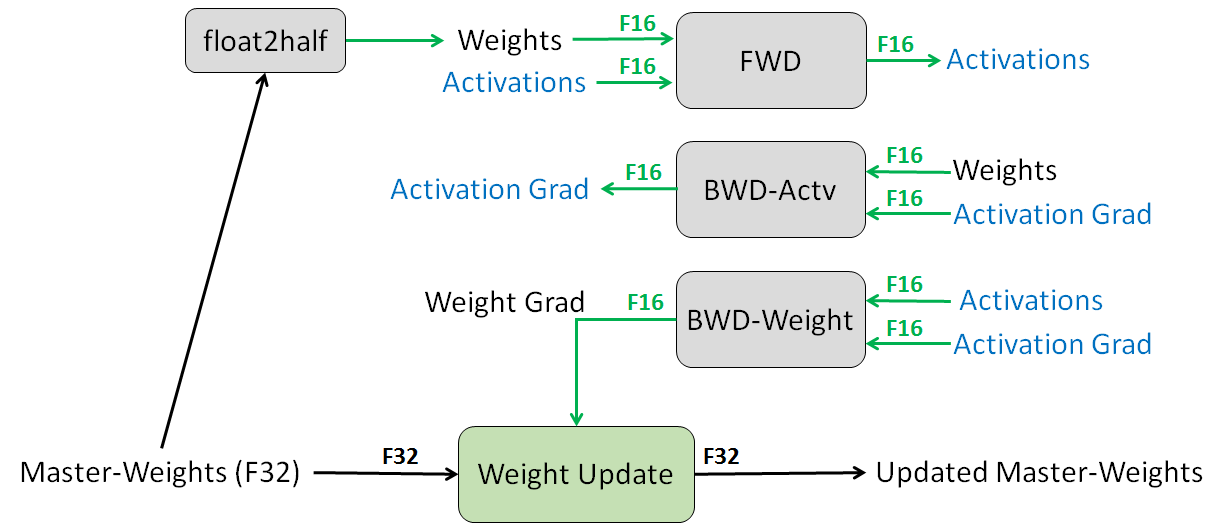
\includegraphics[width=\columnwidth]{img/Background/mixed_prec_iteration.png}
    \caption{FP16 训练流程}
    \label{img::background::fp16_ops}
  \end{subfigure}
  \quad
  \begin{subfigure}[t]{0.45\columnwidth}
    \centering
    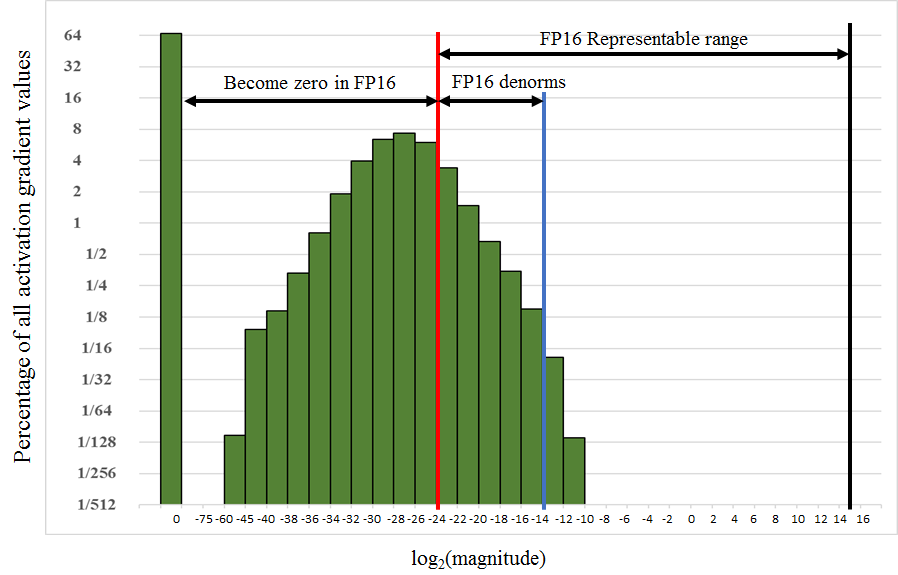
\includegraphics[width=\columnwidth]{img/Background/ssd_ag_log_histo_coarse.png}
    \caption{梯度分布与 FP16 数值范围}
    \label{img::background::fp16_grads}
  \end{subfigure}
  \caption{模型训练时使用 FP16 精度进行前向反向计算,并将梯度缩放后更新底层的 FP32 精度模型参数~\subref{img::background::fp16_ops}。FP16 数值精度有限,需在反传开始前缩放 loss 值以确保梯度计算不会出现数值截断~\subref{img::background::fp16_grads}。图片来自~\citet{micikevicius2018mixed}}
  \label{img::background::fp16_training}
\end{figure}

深度神经网络一般使用单精度浮点存储模型参数和进行数值计算,\citet{micikevicius2018mixed} 指出使用半精度浮点(FP16)也可在不影响模型准确度的前提下将大部分用于不同任务的深度神经网络训练至收敛。FP16 训练流程如图~\ref{img::background::fp16_ops} 所示,在前向传播过程中,模型参数和输入激活被截断转换至 FP16,之后通过 FP16 数值逻辑计算得出输出激活;在反向传播过程中,以 FP16 表示的梯度与以 FP16 缓存的前向过程临时变量通过 FP16 数值逻辑计算得出模型参数和输入激活的梯度,并继续以链式法则进行反向传播。模型参数梯度就绪后,转换至 FP32 格式对实际保存的 FP32 模型参数进行更新。注意如图~\ref{img::background::fp16_grads} 所示,由于 FP16 数值范围有限,幅度值较小的梯度在计算时可能会下溢为 0,因此需要在反向传播开始前适当缩放损失函数值 $\mathcal{L}$,使反向传播中所有梯度保持在 FP16 数值范围内;在将梯度转换至 FP32 时,再将梯度范围缩放至原有数值。

在大部分现代 GPU 及其他包含浮点计算单元的硬件上,同一设备的 FP16 算力一般是 FP32 算力的一倍以上。例如 NVIDIA RTX 2080Ti GPU 的 FP32 算力为 13.45T FLOPS,而其 FP16 算力高达 26.90T FLOPS \citep{nvidia2018turing}。除~\citet{micikevicius2018mixed} 外,\citet{abadi2016tensorflow, dean2012large} 也报告了使用 FP16 或 BFLOAT16 数值精度进行深度神经网络训练的结果。在实际应用中,FP16 一般能将模型训练时间缩短一倍左右。

\begin{figure}[htb]
  \centering
  \includegraphics[width=0.75\columnwidth]{img/Background/int8_training.pdf}
  \caption{INT8 训练对前向过程和反向过程的修改,图片来自~\citet{zhu2019towards}}
  \label{img::background::int8_training}
\end{figure}

另一个更激进的方法是将网络前向、后向传播中的参数、激活量化至带缩放因子的整数张量,从而将模型训练中计算量的大部分替换为整数数值逻辑(图~\ref{img::background::int8_training})。例如,\citet{das2018mixed} 报告了使用 INT16 数值精度训练深度卷积网络,可在不损失模型准确度的情况下获得 $1.8\times$ 训练吞吐量提升;\citet{zhu2019towards} 通过调整量化函数截断阈值和修改模型训练策略,可以在 INT8 数值精度下将 MobileNet~\citep{howard2017mobilenets, Sandler_2018} 系列模型训练收敛,且在 NVIDIA GTX 1080Ti GPU 上实际达到 $+22\%$ 的训练速度提升。

针对分布式训练中各节点间梯度同步问题,目前主要有两种加速方案。一种是使用梯度稀疏化、梯度量化、梯度信息编码等方式减少节点间的通讯量。例如 \citet{wen2017terngrad} 将节点间梯度三值化为 $\{-1, 0, 1\}$,并在不超过 $2\%$ 准确度损失的情况下将 GoogLeNet~\citep{szegedy2015going} 训练至收敛;\citet{aji2017sparse, lin2018deep} 通过幅度阈值对通讯梯度做稀疏化,\citet{lin2018deep} 报告了将 ResNet-50 训练梯度从 97MB 压缩至 0.35MB 而不损失模型准确度。另一种是利用反向传播逐层计算的特性,在模型计算某一层梯度时,同步以就绪的其他梯度,以实现“隐藏”通信时间的效果。\citet{abadi2016tensorflow, paszke2019pytorch} 利用 CUDA stream 异步执行的特性,将 NCCL~\citep{jeaugey2017nccl} 的通信原语与 cuDNN~\citep{chetlur2014cudnn} 的计算操作按调用顺序传递至训练 GPU 的 CUDA stream 中,从而实现对通信开销的隐藏。\citet{peng2019generic} 通过对神经网络不同层间通信的优先级调度以及根据集群网络环境对通信算法参数的优化,在 Parameter Server~\citep{li2014scaling}、基于 all-reduce 的同步训练等分布式训练范式上均获得了显著加速。
% ------------------------------------------------------------------------------
%    Efficient deployment
% ------------------------------------------------------------------------------
\subsection{高效模型部署方法}
神经网络模型在部署时主要面临的挑战仍然是其过高的存储和推理计算开销。为减轻算法模型对计算资源的需求,提高计算资源的利用率,高效模型部署技术的发展主要分为两个方向:从\emph{算法}层面减少部署模型的存储和推理复杂度,从\emph{系统}层面根据部署环境优化模型推理运行时对计算资源的利用率。

\begin{figure}[htb]
  \centering
  \includegraphics[width=0.75\columnwidth]{img/Background/deep_compression.pdf}
  \caption{DeepCompression 部署流程,图片来自~\citet{han2015deep}}
  \label{img::background::deep_compression}
\end{figure}

近年来从算法层面提升模型部署运行效率的工作,几乎都可以归类至 \citet{han2015deep, han2017efficient} 提出的 DeepCompression 框架内(图~\ref{img::background::deep_compression})。DeepCompression 对模型部署的优化加速包含三个流程:通过\emph{剪枝}(pruning)技术减少模型参数量,通过\emph{量化}(quantization)技术降低模型参数和激活数值位宽,最后通过其他无损压缩技术进一步减小模型部署后的体积。剪枝技术主要包括:
{
  \setlist[enumerate]{}
  \begin{enumerate*}[1)]
    \item 非结构化剪枝~\citep{han2015learning},即通过一定标准将模型中参数值置为 $0$ 而提高模型稀疏度,在支持稀疏操作的专有硬件上可降低能耗、提高推理效率;
    \item 结构化剪枝~\citep{li2016pruning},即删除模型卷积层中的部分卷积核和全连接层中的部分通道,可直接地减小模型的存储和计算复杂度;
    \item 层级剪枝~\citep{chen2018shallowing},直接删除网络模型中的部分冗余层。
  \end{enumerate*}
}
模型部署时的量化技术主要包括:
{
  \setlist[enumerate]{}
  \begin{enumerate*}[1)]
    \item 将模型参数量化或二值化至低比特表示~\citep{courbariaux2015binaryconnect, hou2018loss},从而减少模型部署后体积;
    \item 将模型参数和激活同时量化至低比特~\citep{rastegari2016xnor, jacob2018quantization},从而利用整数数值逻辑加速模型部署后的推理过程。
  \end{enumerate*}
}
DeepCompression 流程最后一步使用 Huffman 编码~\citep{van1976construction} 进一步减小模型体积。其他压缩加速算法还包括模型参数的低秩分解~\citep{sainath2013low}、高效矩阵乘法~\citep{lavin2016fast} 等。

\begin{figure}[htb]
  \centering
  \includegraphics[width=0.75\columnwidth]{img/Background/tvm_stack.pdf}
  \caption{TVM 部署系统架构,图片来自~\citet{chen2018tvm}}
  \label{img::background::tvm}
\end{figure}

从系统层面提高模型部署效率的代表性工作是 TVM~\citep{chen2018tvm}。在模型训练并压缩完成后,TVM 首先根据算子融合、内存布局重排列策略,在不改变模型输入——输出映射的情况下对模型进行\emph{计算图重写};随后 TVM 将计算图编译为与硬件无关的\emph{张量表达式},并根据部署环境对张量表达式进行并行化、循环展开、访存延时隐藏等优化,得到最优的\emph{调度策略};之后 TVM 根据模型调度策略和张量表达式生成\emph{字节码},并在部署硬件上实际测试字节码性能,并以此为反馈重新调节调度策略和字节码生成流程,最终在目标硬件上实现神经网络模型的高效部署。
% ==============================================================================
%  Quantized Neural Networks: Algorithms, Softwares and Hardwares
% ==============================================================================
\section{量化神经网络}
量化神经网络~\citep{guo2018survey} 及其特例二值化神经网络~\citep{qin2020binary} 通过将神经网络模型参数、激活、梯度使用特定方法压缩至低比特定点数、整数,或根据某一查找表进行映射至离散值(例如根据数值符号和阈值映射至 $\{-1, 0, 1\}$ ),达到减少模型参数体积(量化模型参数)、加速模型运算(同时量化模型参数和激活)及减少模型分布式训练通信量(量化模型梯度)的目的。具体地,给定一待量化输入 $x\in \mathbb{R}$,量化函数 $Q(\cdot)$ 将其映射至一离散集合 $\mathbb{T}$ 中的对应值,即 $\hat{x} = Q(x): \mathbb{R} \to \mathbb{T}$;在反向传播阶段,则根据相应的求导原则 $\diff{\hat{x}}{x}$ 将上游梯度 $\diff{\mathcal{L}}{\hat{x}}$ 传递至 $x$ 以继续梯度的链式法则计算。近年来量化神经网络领域大量工作主要集中探讨两个话题:量化函数 $Q(\cdot)$ 的设计方式,以及在给定量化函数后对量化模型 $\QuantNet$ 的优化方法。本节将依次介绍量化函数设计和量化函数优化方面的代表性工作。最后,本节还将介绍用于训练部署量化神经网络的软件和硬件实现。
% ------------------------------------------------------------------------------
%    Quantizers
% ------------------------------------------------------------------------------
% ○ Quantizers
%   § BinaryConnect
%   § BNN
%   § XNOR-Net
%   § DoReFa
%   § HWGQ
%   § PACT
%   § ABC-Net
%   § LQ-Nets
%   § APoT
% ○ Training methods
%   § QAT
%     □ Integer-only
%     □ Distillation Quantization / Apprentice
%     □ Loss-aware binary/ternary
%     □ LR-Nets / Probabilistic BNN
%     □ LIQ
%     □ DSQ
%   § Post-training methods
%     □ WhitePaper
%     □ Few-data calibration
%     □ Data-free / same but different
%   § Allocate the bit budget
%     □ AutoML methods (HWQ)
%     □ Metric-based methods (Hessian aware quant)
\subsection{量化函数设计}
BinaryConnect~\citep{courbariaux2015binaryconnect} 是最早使用量化技术减少模型参数体积的工作。在前向传播时,BinaryConnect 根据模型参数 $w$ 的幅度大小,\emph{随机地}将其映射至 $\{-1, 1\}$;在反向传播过程中,使用 Straight Though Estimator (\citet{bengio2013estimating},下文简称 STE) 将量化函数的上游梯度直接复制至全精度输入。为防止模型参数由于前向过程中幅度信息 $|w|$ 丢失而造成过多偏移,每步参数更新会将参数范围限制在 $[-1, 1]$ 之间。具体地,
\begin{align}
  \text{\textbf{Forward}: } & \hat{w} = 
    \begin{cases}
      1 & \text{ with probability } p = \hat{\sigma}(w) \\
      -1 & \text{ with probability } 1 - p
    \end{cases} \\
  \text{\textbf{Backward}: } & \diff{\mathcal{L}}{w} = \diff{\mathcal{L}}{\hat{w}} \label{eq::background::ste}
\end{align}
其中 $\diff{\mathcal{L}}{\hat{w}}$ 为损失函数 $\mathcal{L}$ 传导至 $\hat{w}$ 处的梯度,$\hat{\sigma}(w) = \max(0, \min(\frac{w+1}{2}, 1))$。在使用 $\diff{\mathcal{L}}{w}$ 更新 $w$ 后,再将 $w$ 范围限制在 $[-1, 1]$ 之间。

Binarized Neural Networks (\citet{hubara2016binarized}, 下文简称 BNN) 进一步将模型激活也映射至 $\{-1, 1\}$,以便使用\emph{算术位移}操作完成模型的前向传播。为减轻模型前向传播的计算开销,BNN 使用确定性量化处理模型激活:
\begin{align}
  \text{\textbf{Forward}: } & \hat{x} = 
    \begin{cases} 
      1 & \text{ if } x \ge 0 \\
      -1 & \text{ otherwise}
    \end{cases}
    \label{eq::background::sign}
\end{align}
同时 BNN 也提出了使用算术位移实现的 Batch normalization~\citep{ioffe2015batch} 和 AdaMax~\citep{kingma2014adam},并报告上述基于位移的实现在 GPU 上可节省 $60\%$ 的模型推理时间。

为进一步提高量化参数 $\hat{w}$ 针对全精度参数 $w$ 的近似准确性,XNOR-Net \citep{rastegari2016xnor} 为量化参数引入了浮点缩放 $\alpha$,并将量化过程视为针对量化后参数和缩放的最小二乘问题:
\begin{align}
\arg\min_{\hat{w}, \alpha} &= \| \alpha\hat{w} - w \|_2 \label{eq::background::xnor_opt}
\end{align}
\eqref{eq::background::xnor_opt} 存在闭式解 $\alpha^* = \frac{\|w\|_1}{n}$,$\hat{w}^* = \sign(w)$,其中 $n$ 为参数张量 $w$ 中所含元素个数,$\sign$ 即为 \eqref{eq::background::sign}。

值得注意的是,在 BNN 和 XNOR-Net 中,量化后的激活 $\hat{x}$ 和参数 $\hat{w}$ 满足 $\hat{x}, \hat{w} \in \{-1, 1\}$,因此它们之间的点积操作可用异或(XNOR)及 1-位计数(bitcount)完成:
\begin{align}
  \hat{x} \cdot \hat{w} &= N - 2 \cdot \mathrm{bitcount}(\mathrm{xnor}(\hat{x}, \hat{w})) \label{eq::background::xnor_dot}
\end{align}
其中 $N$ 为向量 $\hat{w}, \hat{x}$ 中所含元素个数。

DoReFa-Net~\citep{zhou2016dorefanet} 引入了 k-bit 量化函数 $Q_k(\cdot)$,使得量化点集 $\mathbb{T}$ 中可用元素数目达到了 $2^k-1$。具体地,给定一全精度输入 $x\in [0, 1]$,k-bit 量化函数定义为:
\begin{align}
  \text{\textbf{Forward}: } & \hat{x} = \frac{\lfloor (2^k - 1)x \rceil}{2^k - 1} \label{eq::background::dorefa_fwd} \\
  \text{\textbf{Backward}: } & \diff{\mathcal{L}}{x} = \diff{\mathcal{L}}{\hat{x}}
\end{align}
其中 $\Round{\cdot}$ 为舍入操作符。对于模型参数 $w$,DoReFa-Net 使用 $\tanh$ 函数将其映射至 $[-1, 1]$,再线性映射至 $Q_k(\cdot)$ 的定义域内;对于经过非线性层后的模型激活 $x$,则直接将其截断至 $[0, 1]$;对于梯度 $g$ 的处理方式和 $w$ 类似,但是会在量化前叠加幅度范围在 $\pm \frac{|g|}{2}$ 之内的均匀噪声。

Half Wave Gaussian Quant (\citet{cai2017deep},下文简称 HWGQ)注意到非线性层之后的模型激活 $x$ 通常符合从 0 截断的半波高斯分布,故使用分段式函数定义 $Q(\cdot)$。在给定量化位宽 $k$ 之后,
\begin{align}
  \text{\textbf{Forward}: } & \hat{x} = 
    \begin{cases} 
      q_i & \text{ if } x \in (t_i, t_{i+1}] \\
      0 & \text{ } x \le 0
    \end{cases}
    \label{eq::background::hwgq}
\end{align}
其中 $\{q_1, \ldots q_{2^k-1}\}$ 为量化点集,$t_0=0, t_1, \ldots, t_{2^k-1}, t_{2^k}=\infty$ 为分段函数的边界。$\{q_i, t_j\}, i, j \in {1, \ldots 2^k-1}$ 的取值通过 Lloyd~\citep{lloyd1982least} 算法求解优化问题
\begin{align}
  \arg\min_{q_i, t_j} \|\hat{x} - x\|_2
\end{align}
得出。

PArameterized Clipping acTivation (\citet{choi2018pact} 下文简称 PACT),为减少模型激活量化误差,设计了带可学习上界参数 $\beta$ 的线性截断函数代替 ReLU,并将截断后的激活值线性缩放至 $[0, 1]$ 之后传入 \eqref{eq::background::dorefa_fwd} 中。在模型反向传播过程中,$\beta$ 使用接收到的梯度进行更新。 

DoReFa-Net 和 PACT 所用的 k-bit 线性均匀量化函数 \eqref{eq::background::dorefa_fwd} 实际是将量化后的 $\hat{x}$ 表示为其编码向量 $b_x = [b_1, \ldots b_k], b_i \in \{0, 1\}$ 与 2-幂基底 $v^{(2)} = [2^0, 2^1, \ldots 2^{k-1}]$ 和缩放因子 $\alpha$ 的点积,即 $\hat{x} = \alpha v^{(2)} b_x^T$。LQ-Nets~\citep{Zhang_2018} 指出量化函数所用基底可以不一定是 2-幂基底 $v^{(2)}$,而可以在训练过程中学习适合目标网络数值特性的基底 $v = [v_1, \ldots, v_k], v_i \in \mathbb{R}$。由基底 $v$ 同样可以在 k-bit 编码上生成 $2^k$ 个量化点 $[q_1, \ldots, q_{2^k}]$,其中 $q_1 = v [0, \ldots 0]^T, q_{2^k} = v [1, \ldots 1]^T$。具体地,LQ-Nets 所用量化函数 $\hat{x} = Q_{\mathrm{LQ}}(x, v)$ 实现为
\begin{align}
  \text{\textbf{Forward}: } & \hat{x} = v b_x^T \label{eq::background::lq_fwd}
\end{align}
其中 $b_x$ 为 $q_i \le x < q_{i+1}$ 时 $i$ 对应的编码向量。使用 \eqref{eq::background::lq_fwd} 对实数向量点积 $wa^T, w, a \in \mathbb{R}^N$ 操作数量化后,点积操作可以用 \eqref{eq::background::xnor_dot} 在 $w, a$ 的编码向量上完成,即
\begin{align}
  Q_{\mathrm{LQ}}(w, v^{(w)}) Q_{\mathrm{LQ}}(a, v^{(a)})^T &= \sum_{i=1}^{k_w} \sum_{j=1}^{k_a} v^{(w)}_i v^{(a)}_{j} (b^{(w)}_i b^{(a)}_j)
\end{align}
其中 $k_w, k_a$ 分别为操作数 $w, a$ 的量化位宽,$v^{(w)} \in \mathbb{R}^{k_w}, v^{(a)} \in \mathbb{R}^{k_a}$ 为 $w, a$ 在 LQ-Nets 量化模式中的基底,$b^{(w)}, b^{(a)}$ 间的点积可以由 \eqref{eq::background::xnor_dot} 完成。

\begin{figure}[htb]
  \centering
  \includegraphics[width=\columnwidth]{img/Background/APoT.pdf}
  \caption{在 $[0, 1]$ 范围内,APoT 量化方式(右)与均匀量化(左)和 2-幂量化(中)的对比。图片来自 \citet{li2019additive}}
  \label{img::background::apot}
\end{figure}

Additive Power-of-Two (\citet{li2019additive},下文简称 APoT)将量化位宽 $k$ 拆分为 $n$ 个位宽为 $m$ 的 2-幂量化子项,将输入编码为 $n$ 个子项的加和,以避免普通 2-幂量化的量化点过于集中在零点附近的问题。具体地,在给定实数输入 $x\in [0, \alpha)$ 后,其量化函数 $\hat{x} = Q_{\mathrm{APoT}}(x; \alpha, m, n)$ 实现为:
\begin{align}
  Q_{\mathrm{APoT}}(x; \alpha, m, n) &= \gamma \times \{ \sum_{i=0}^{n-1} p_i \} \\
  \text{where } p_i &\in \{0, \frac{1}{2^i}, \frac{1}{2^{i+n}}, \ldots \frac{1}{2^{i + 2^{m-1}n}}\} \notag
\end{align}
其中 $\gamma$ 为缩放因子,确保 $Q_{\mathrm{APoT}}(x; \alpha, m, n)$ 输出的最大项数值为 $\alpha$,各项位宽 $m$ 和项数 $n$ 满足 $k = mn$。在 $\alpha = 1, m = n = 2$ 时,APoT 量化方式与其他常见量化方式的对比见图~\ref{img::background::apot}。
% ------------------------------------------------------------------------------
%    Training methods
% ------------------------------------------------------------------------------
\subsection{量化模型优化方法} \label{sec::background::train_qnn}
一般神经网络模型在量化后会遭受准确度损失,因此需要使用特定方法恢复量化模型的准确度。目前量化模型的优化方法主要分两类:需要在特定数据集上进行前向传播和反向传播计算,使用得到的梯度更新模型参数的\emph{量化感知训练}(\emph{Quantization-aware Training},下文简称 QAT)方法;以及不需要反向传播计算,在使用少量数据或完全没有训练数据情况下,进行模型量化参数标定及其他操作即可完成转换部署的\emph{量化后处理}(\emph{Post-training Quantization},下文简称 PTQ)方法。

\begin{figure}[htb]
  \centering
  \includegraphics[width=0.75\columnwidth]{img/Background/qat_ptq.png}
  \caption{TensorFlow Lite 中模型参数量化(左)、量化后处理方法(中)和量化感知训练方法(右)的算法流程。图片来自~\citet{krishnamoorthi2018quantizing}}
  \label{img::background::qat_ptq}
\end{figure}

PTQ 方法包含对模型激活的标定,对模型正则化参数的调整,以及在不使用梯度信息的情况下对模型参数进行微调。由于各类量化函数运行前需获知被量化输入的数值范围,故对神经网络模型参数、激活同时量化时,需要确定模型各层激活数值范围,即对模型激活进行\emph{标定}。TensorFlow Lite 的 PTQ 模块~\citep{abadi2016tensorflow, krishnamoorthi2018quantizing} 在标定数据集上运行待量化的模型,记录模型中每层参数的最大最小值,并通过动量 $M$ 以指数移动平均(Exponential Moving Average)方式更新每层激活的量化范围(图~\ref{img::background::qat_ptq} 中间部分流程)。\citet{he2018learning, peters2018probabilistic} 指出原模型中 BN 等正则化层的统计参数并不能有效地匹配量化模型的激活分布,因此提出在标定数据集上运行量化后的模型时,应根据量化激活的分布情况重新统计并更新模型中的正则化参数。在无法接触到训练数据或标定数据的情况下,\citet{nagel2019data, meller2019same} 通过调整量化模型参数分布,在不改变模型输入——输出映射关系的前提下减少模型量化误差,恢复量化模型准确度。

QAT 方法与一般神经网络训练方法类似,将量化后的模型在训练集上进行前向传播和反向传播计算,并按照特定策略对模型参数进行梯度下降更新(图~\ref{img::background::qat_ptq} 右侧流程)。QAT 方法的主要问题是量化函数对于量化输入并不可导,各类工作针对此问题提供了不同的解决方案:模型量化的早期工作 \citet{courbariaux2015binaryconnect, hubara2016binarized, rastegari2016xnor, zhou2016dorefanet} 使用 STE~\eqref{eq::background::ste} 将量化函数输出接受的梯度直接复制至其输入,以确保链式法则能继续进行。由于量函数的全精度输入与求导时所用的量化输出数值并不一定相同,所以使用 STE 反传梯度会出现梯度不匹配问题,且在量化数值精度较低时更为明显。为解决此问题,\citet{cai2017deep} 探索了 HWGQ 量化函数的可微分导数近似;\citet{louizos2018relaxed} 使用可微分的 Gumbel Softmax~\citep{jang2016categorical, maddison2016concrete} 算子,在全精度模型的训练过程中逐渐将模型参数和激活由连续分布“硬化”至离散分布;\citet{gong2019differentiable} 提出的 Differentiable soft quantization 算子将分段函数的导数使用可微分的类 $\tanh$ 函数近似,并在训练过程中逐渐接近实际分段函数。除改进 STE 的梯度准确度外,其他实现高精度 QAT 的方法包括:\citet{peters2018probabilistic, shayer2018learning} 将神经网络的量化操作视为随机过程,即量化后的参数或激活服从特定的参数化离散分布,在反向传播时即可针对分布参数求导;\citet{hou2016loss, hou2018loss} 利用 Adam 优化算法~\citep{kingma2014adam} 中的二阶动量信息作为 Hessian 近似,使用拟牛顿法直接对模型量化权重的缩放因子 $\alpha_w$ 和量化表示 $b_w$ 求导并优化;\citet{polino2018model, mishra2018apprentice} 使用知识蒸馏技术~\citep{hinton2015distilling} 将高准确度大模型的输出作为“软标签”引入 QAT 过程,以改善量化模型的准确度;\citet{jung2019learning} 使用参数化的量化函数,并在 QAT 阶段将量化函数参数引入模型任务损失计算,以此通过模型反向传播时的梯度优化量化函数。
% ------------------------------------------------------------------------------
%    Softwares and hardwares
% ------------------------------------------------------------------------------
\subsection{相关软硬件实现}
现今大量底层数学计算库已支持整数通用矩阵乘法(integer general matrix multiplication,下文简称 IGEMM)以及整数卷积计算(integer convolution,下文简称 ICONV):gemmlowp~\citep{google2018gemmlowp}、qnnpack~\citep{facebook2018qnnpack}、fbgemm~\citep{facebook2018fbgemm}、DNNL~\citep{intel2019dnnl} 支持 INT8 数值精度的 IGEMM 及 ICONV 操作,cuBLAS~\citep{nvidia2008cublas}、CUTLAS~\citep{nvidia2019cutlass} 和 cuDNN~\citep{chetlur2014cudnn} 在包含 TensorCore~\citep{nvidia2018turing} 的 NVIDIA GPU 上支持 FP16、INT8、INT4 精度的 IGEMM 和 ICONV 操作。

在底层计算库加持下,目前的主流神经网络软件框架已支持量化神经网络的训练和部署:TensorFlow Lite~\citep{abadi2016tensorflow} 借助 gemmlowp 支持以 PTQ、QAT 方式转换和训练 INT8 量化神经网络,并通过 Android Neural Networks API~\citep{google2020neurl} 部署至移动设备;Caffe2~\citep{markham2017caffe2}、PyTorch~\citep{paszke2019pytorch} 通过 fbgemm 支持 INT8 神经网络在 x86 平台上的量化推理和 GPU 平台上的 QAT,并通过 qnnpack 支持将模型部署至移动端;onnx~\citep{onnx2019onnx} 在计算图规范中包含了线性量化、反量化等操作,能够作为量化神经网络的通用中间表示。

在量化神经网络通过 PTQ 或 QAT 训练完成并转换为 onnx 中间表示后,可通过不同工具软件进行部署至相应平台:TensorRT~\citep{migacz20178} 自身包含 PTQ 能力,支持将模型部署至包含 TenosrCore 的 NVIDIA 硬件上;Core ML~\citep{apple2020coreml} 支持将模型部署至包含 Apple Neural Engine 的移动设备上;SNPE~\citep{qualcomm2019snpe} 自身包含基于激活标定和 data-free quantization 的 PTQ 能力,支持将模型部署至包含 DSP 或 AIX 的 Qualcomm 移动设备上。
% ~~~~~~~~~~~~~~~~~~~~~~~~~~~~~~~~~~~~~~~~~~~~~~~~~~~~~~~~~~~~~~~~~~~~~~~~~~~~~~
%  FQN
% ~~~~~~~~~~~~~~~~~~~~~~~~~~~~~~~~~~~~~~~~~~~~~~~~~~~~~~~~~~~~~~~~~~~~~~~~~~~~~~
\chapter{用于目标检测的全量化网络} \label{chap::fqn}
% ==============================================================================
%  Introduction
% ==============================================================================
\section{引言}
正如第~\ref{chap::background} 章所介绍,基于深度学习的目标检测技术已在大量真实世界的任务上取得显著成功 \citep{lecun2015deep}。然而,高昂的运算和存储开销,是将目标检测技术广泛应用到诸如智能手机、智能安防相机、自动驾驶系统等计算资源受限场景的主要障碍。为减少深度学习模型的运算和存储开销,近年来学术界和工业界探索了多种解决路径,其中主要方向包括高效的模型算子和结构探索~\citep{howard2017mobilenets, Sandler_2018, iandola2016squeezenet, zhang2018shufflenet}、以部署平台模型推理时间为约束的模型结构自动搜索~\citep{wu2019fbnet, tan2019mnasnet, tan2019efficientnet}、模型剪枝~\citep{han2015learning, li2016pruning, chen2018shallowing} 和模型量化~\citep{rastegari2016xnor, zhou2016dorefanet, jacob2018quantization} 等。其中,模型量化技术由于可以显著减少模型尺寸,同时使用更高效的整数或定点运算逻辑代替一般深度学习模型所需的浮点运算逻辑而提高推理效率,近年来受到了较多关注,也是本章讨论的重点。

现有的模型量化技术在物体分类等相对简单的任务上表现出色~\citep{zhou2016dorefanet, Zhang_2018, li2019additive},然而将其应用到目标检测~\citep{zou2019object} 这一较为复杂的任务时,会在模型训练及硬件部署时面临额外的挑战:
\begin{enumerate}[1)]
  \item 与只需学习模型输出间偏序关系的分类任务不同,目标检测还需要模型准确地将预设锚框(anchor box)准确地回归至检测物体的边界框(bounding box),低比特量化后的模型可能难以处理这一回归任务;
  \item 检测模型为保持特征图(feature map)的空间信息,其输入图片尺寸较分类任务增大(一般检测模型输入图像短边尺寸为 $600\sim 800$ 像素)而占用更多 GPU 显存,导致训练时单 GPU 批量大小(batch size)缩小至 2 或 4,从而影响模型中部分正则化操作,例如批正则化(Batch Normalization~\citep{ioffe2015batch},下文简称 BN)层的效率,使得本身就难以训练的量化网络更不稳定、难以收敛;
  \item 大部分运行量化模型的专有硬件,例如终端设备上嵌入的 FPGA 和 DSP 等,为保证硬件利用率和访存效率,并不包含浮点运算单元。这要求量化检测模型在训练后不包含任何浮点操作,而现有的大部分模型量化算法~\citet{zhou2016dorefanet, Zhang_2018, li2019additive} 为保证模型量化后准确度,会将模型的 BN 层等敏感部分数值精度保留为浮点。同时,一些模型量化方法对一般硬件部署并不友好,例如 \citet{zhu2016trained, cai2017deep}。
\end{enumerate}

针对上述挑战,本章提出了一种适用于目标检测任务且对于一般硬件友好的低比特量化神经网络训练及部署方法,称为\emph{用于目标检测的全量化网络}(\emph{Fully Quantized Network for Object Detection},下文简称 FQN)。FQN 可以在复杂的目标检测模型——例如 RetinaNet~\citep{lin2017focal} 和 Faster RCNN~\citep{ren2015faster} 上——将模型参数及激活的数值精度量化至 4 比特,并保持足够的准确度。FQN 使用对于一般硬件友好的非对称线性量化,且通过 BN 折叠技术,使模型训练后不包含任何浮点操作。为解决 FQN 的训练收敛问题,本章详细分析了其在 MS COCO 数据集~\citep{lin2014microsoft} 上的训练过程,指出其训练不稳定性的根源在于模型参数的通道间分布差异、模型激活量化的准确度不足以及小训练批量尺寸导致的 BN 统计量不稳定,并提出了相应的措施解决上述问题。

本章在 MS COCO 数据集上验证了 FQN 的有效性,所用的检测算法包括一阶检测算法 RetinaNet 和二阶检测算法 Faster RCNN,所用的模型包括使用特征金字塔(Feature Pyramid Network~\citep{lin2017feature},下文简称 FPN)的 ResNet-\{18, 34, 50\}~\citep{He_2016} 和 MobileNet-v2~\citep{Sandler_2018}。FQN 在上述实验中均保持了较高准确度,例如使用 4-bit ResNet-18 的 RetinaNet 检测模型应用 FQN 训练后,其 mAP 相较全精度模型仅下降 $0.031$ (4-bit $0.286$ mAP 相较于全精度 $0.317$ mAP),而之前被用于 TensorFlow Lite 中的 \citet{jacob2018quantization} 和 \citet{krishnamoorthi2018quantizing} mAP 下降分别为 $0.120$ 和 $0.091$,其相对准确度损失是 FQN 的 $3.87\times$ 和 $2.94\times$。
% ------------------------------------------------------------------------------
%    Motivation
% ------------------------------------------------------------------------------
\subsection{工作动机}
\paragraph{对于一般硬件友好的全量化网络}
量化网络的大部分部署场景(包括软件及硬件)并不支持特殊的量化模式,例如 NVIDIA TensorRT~\citep{vanholder2016efficient} 在包含 Tensor Core 的 GPU 或加速卡上运行 8-bit/4-bit 模型时,只支持对称线性量化~\citep{migacz20178},Qualcomm SNPE~\citep{qualcomm2019snpe} 在 DSP 或 AIX 设备上运行 8-bit 模型时,只支持零点对齐的非对称线性量化。这意味着,目前许多使用特殊量化函数的模型量化研究~\citep{zhu2016trained, cai2017deep, Zhang_2018} 是对一般硬件不友好且难以实际部署的。同时,大部分现有研究过于关注量化模型的最终准确度,将量化模型中的敏感操作——例如模型第一层和最后一层、模型中的 BN 等正则化层等——保留为浮点数值精度~\citep{zhou2016dorefanet, Zhang_2018, li2019additive}。在实际的部署场景中,智能相机等终端设备内嵌的 FPGA 或 ASIC 等专有硬件为保证硬件利用率一般不会再额外设计浮点运算逻辑;移动设备端的神经网络推理库虽然支持将模型中部分操作从 DSP 或 AIX 等量化设备回调(fallback execution)至支持浮点运算的 CPU 或 GPU,但其中涉及的上下文切换会极大降低模型的运行效率。因此,探索针对一般硬件友好的、完全量化的模型量化方法有极大的潜在实际影响力。

\paragraph{适用于复杂任务的低比特量化网络}
目前神经网络模型量化研究主要集中在两个方向:
\begin{enumerate}[1)]
  \item 在相对简单的模型、任务和数据集上,使用极低的数值精度量化模型参数及激活。例如 \citet{hubara2016binarized, zhou2016dorefanet} 报告了在 SVHN、CIFAR-10 等物体分类任务上,可将 small-VGG、AlexNet 等模型参数及激活压缩至 1-bit;
  \item 使用较高的数值精度,量化用于相对复杂任务的模型。例如 \citet{jacob2018quantization} 报告了在人脸特征抽取、人脸检测、通用目标检测任务上,多种模型可在 8-bit 精度下保持可用准确度。
\end{enumerate}

由于定点或整数乘法逻辑的计算开销与量化位宽呈超线性,且占计算能耗大部分的访存开销正比于量化位宽~\citep{han2017efficient},8-bit 量化的资源开销对于计算资源非常受限的设备而言仍然过于高昂。因此一个自然的想法是,能否将 4-bit $\sim$ 1-bit 低比特压缩技术用于复杂任务和复杂模型上。然而,直接将 \citet{rastegari2016xnor, zhou2016dorefanet} 等量化训练方法用于复杂模型时,会出现量化训练无法收敛、最终模型准确度低的问题。本章通过观察复杂任务上量化模型的训练过程,发现其中存在 BN 层 EMA 统计值波动明显、量化激活存在较多离群点等不稳定现象。后续实验进一步发现消除这些不稳定性,可显著改善复杂任务上低比特量化模型的训练收敛性并提高模型最终准确度(详见第~\ref{sec::fqn::experiments} 节)。
% ------------------------------------------------------------------------------
%    Contributions
% ------------------------------------------------------------------------------
\subsection{主要贡献}
\begin{enumerate}
  \item 本章提出了 FQN,一种适用于目标检测模型的低比特量化方法。FQN 使用对一般硬件友好的线性量化方式,使量化后的目标检测模型可以使用整数计算逻辑进行推理,且量化后的模型不包含浮点操作,便于部署至计算资源受限的终端设备;
  \item 本章分析了 FQN 的训练过程,指出其在低比特量化训练中不稳定性的主要来源,并提出了相应解决方案;
  \item 本章在 MS COCO 数据集上,使用不同神经网络模型和目标检测算法验证了 FQN 的准确性。FQN 在实验中达到了高于先前领域最优方法的检测准确度。
\end{enumerate}
% ==============================================================================
%  Method
% ==============================================================================
\section{目标检测模型的量化} \label{sec::fqn::methods}
本节详细描述 FQN 方法的各组成部分,包括对目标检测模型参数和激活的量化算法、量化模型的训练策略以及针对检测模型量化的实现细节。FQN 通过量化感知训练,可使检测模型在以低至 4-bit 的数值精度运行时仍保持足够的准确度。低比特量化目标检测模型的难点在于量化感知训练的不稳定性,而 FQN 通过对模型参数、激活、正则化层的量化算法和训练策略的改进以减少该不稳定性。FQN 对模型参数和激活使用线性量化,量化后仅需整数数值逻辑即可完成模型推理,从而便于部署至一般硬件平台上。
% ------------------------------------------------------------------------------
%    Quantization aware training
% ------------------------------------------------------------------------------
\subsection{量化感知训练} \label{sec::fqn::qat_overview}
根据~\citet{krishnamoorthi2018quantizing} 提出的针对模型量化方法的分类标准,FQN 属于\emph{量化感知训练}(\emph{Quantization Aware (re-)Training},下文简称 QAT),即在模型训练时将模型参数及激活按照部署时的量化方式映射至离散浮点值,以模拟模型量化运行时的数值误差,从而训练得到在量化误差存在时仍能在目标任务上保持足够准确度的模型。采用 QAT 的模型量化训练部署流程依次包含下三个阶段:
\begin{description}
  \item[模型预训练] 在没有预先提供全精度预训练参数时,需要对模型进行预训练。对于物体分类等相对简单的任务,模型在以特定方式初始化后直接在目标数据集上训练;对于目标检测、场景分割等相对复杂的任务,则一般先将其主干模型(backbone network)在分类任务上训练至收敛,再加入任务子模型在目标数据集上训练。模型参数和激活在预训练过程中保持全精度。对于包含 BN 等正则化操作的模型,模型每层在训练时会统计在当前的小批量输入下,该层输出各通道的均值、方差 $\{\Batch{\mu}, \Batch{\sigma}\}$,使用该组统计值将其输出正则化为近似标准高斯分布,并通过动量 $m$ 更新该层输出均值、方差的指数移动平均(Exponential Moving Average,下文简称 EMA)统计值 $\{\EMA{\mu}, \EMA{\sigma}\}$;
  \item[模型量化感知训练] 在模型预训练结束,或事先已获得全精度预训练模型后,则对该全精度模型进行量化感知训练。量化感知训练在模型计算图中加入额外算子:对于模型各层参数和激活,在前向传播时将其离散化,以模拟量化部署运行时的数值误差;在反向传播时,则通过 Straight Though Estimator (下文简称 STE,详见第~\ref{sec::fqn::q_weight} 节)或其他方法,根据算子离散输出接收的梯度计算出其全精度输入的梯度,以便继续梯度传播。注意在此阶段,每组模型参数均保留一份全精度副本,以确保参数能被数值范围较小的梯度准确更新。
  
  在此阶段,先前基于 QAT 的主要工作~\citet{jacob2018quantization, krishnamoorthi2018quantizing} 在量化后的模型激活上计算其小批量统计值 $\{\Batch{\mu}, \Batch{\sigma}\}$ 并继续更新各层 EMA 统计值 $\{\EMA{\mu}, \EMA{\sigma}\}$。我们发现这是导致目标检测模型 QAT 不稳定的原因之一,详见第~\ref{sec::fqn::q_bn} 节;
  \item[模型量化部署] 在上一阶段完成后,所得模型已经可以在量化误差下保持足够准确度。在模型部署前,需将模型中 BN 层的参数——其 EMA 统计值 $\{\EMA{\mu}, \EMA{\sigma}\}$ 和仿射参数 $\{\alpha, \beta\}$ ——合并至前一层卷积或全连接层的参数 $\{W, b\}$ 中,消除额外的线性操作以提高模型推理效率。之后将模型中所有参数转换至部署平台所支持的量化格式,例如包含以 \verb|int32| 定点数表示量化缩放的 \verb|uint8| 矩阵,最终在目标平台上运行。注意量化后的模型也可以在 GPU 上以离散浮点形式使用 \verb|cuDNN| 等浮点计算库运行,以快速验证 QAT 后量化模型的准确度。
\end{description}
% ------------------------------------------------------------------------------
%    Asymmetric linear quantization
% ------------------------------------------------------------------------------
\subsection{非对称线性量化} \label{sec::fqn::quant_scheme}
目前大多数神经网络模型使用单精度浮点格式存储其模型参数,并在运行时使用浮点数值逻辑计算中间激活和最终输出。模型量化方法将这些浮点值舍入至事先定义的一组离散数值中,以减少模型的存储开销;若这些离散数值以线性均匀或 2 的幂次均匀(power-of-two uniform)排布,则运行时的计算可在离散数值的\emph{秩}上以整数数值逻辑进行。具体地,给定一浮点格式的张量 $X^R = [x^R_{1, \ldots n}]$ 和量化位宽 $k$,量化函数 $Q_k(\cdot)$ 将每一浮点值 $x^R_i$ 映射至距其最近的量化点 $q_j$:
\begin{align}
  X^Q = Q_k(X^R) \in \{q_1, \ldots q_{2^k-1}\} 
\end{align}

FQN 使用\emph{非对称线性量化}模式,即任意相邻 $q_j, q_{j+1}$ 间等距,但 $\{q_0, \ldots q_{2^k-1}\}$ 不关于零点对称。因此在 FQN 中,$X^Q$ 按照
\begin{align}
  X^Q = \Delta (X^I - z) \label{eq::fqn::asymm_linear_q}
\end{align}
计算得出。其中 $\Delta$ 表示任意 $q_j, q_{j+1}$ 间的距离(下文统称\emph{量化间距}),$X^I$ 是以无符号整数表示的、 $X^R$ 中各元素在量化点集中的秩,$z$ 表示实数零点对应至量化点集的秩。在给定量化数值范围 $[lb, ub]$ 和量化位宽 $k$ 后,$\Delta$ 按照
\begin{align}
  ub &= \max(ub, lb + \epsilon) \\
  \Delta &= \frac{ub - lb}{2^k - 1}
\end{align}
计算得出。其中 $\epsilon$ 为确保数值稳定性而设置的最小量化范围,一般设为 $10^{-2}$,且给定量化范围后 $q_1 = lb$,$q_{2^k-1} = ub$。在得到 $\Delta$ 后,$X^I$ 可按照
\begin{align}
  \tilde{X}^R &= \Clamp{X^R, lb, ub} \\
  X^I &= \Round{\frac{\tilde{X}^R - lb}{\Delta}}
\end{align}
计算得出。其中 $\Clamp{\cdot, a, b} = \max(a, \min(\cdot, b))$,将输入 $X^R$ 限制在量化范围内;$\Round{\cdot}: \mathbb{R}\to\mathbb{Z}$ 为舍入操作符。

当模型第 $l$ 层的参数 $W_l$ 和输入 $x_l$ 均被量化后,其数值操作变为
\begin{align}
  y_l = Q_k(W_l) Q_k(x_l) = \Delta_{W_l}\Delta_{x_l} (W^I_l x^I_l) \label{eq::fqn::intmm}
\end{align}
由于 $W^I_l, x^I_l$ 均以无符号整数表示,该层的数值运算可用更为高效的整数数值逻辑进行。注意~\eqref{eq::fqn::intmm} 中省略了对零点 $z$ 的处理,以及使用非浮点数值逻辑处理 $\Delta_{W_l}\Delta_{x_l}$ 的讨论。关于零点和缩放的算法及部署细节的详细讨论见第~\ref{sec::fqn::q_misc} 节。% 和第~\ref{sec::fqn::deployment} 节。

因为包含舍入操作 $\Round{\cdot}$ 的量化函数 $Q_k(\cdot)$ 并不可导,因此 FQN 在训练时使用 STE~\citep{bengio2013estimating} 回传上游梯度 $\diff{y}{X^I}$。注意超出量化范围 $[lb, ub]$ 的输入元素不接收梯度:
\begin{align}
  \diff{y}{x^R_i} = 
    \begin{cases}
      \diff{y}{x^I_i} & \text{if } x^R_i \in [lb, ub] \\
      0 & \text{otherwise}
    \end{cases}
\end{align}
% ------------------------------------------------------------------------------
%    Quantize weights
% ------------------------------------------------------------------------------
\subsection{模型参数量化} \label{sec::fqn::q_weight}

\begin{figure}[htb]
  \centering
  \begin{subfigure}[t]{0.45\columnwidth}
    \centering
    \includegraphics[width=\columnwidth]{img/FQN/res50_channels.pdf}
    \caption{ResNet-50 模型参数各通道间最大/最小幅度比值的柱状统计,注意 x 轴单位为分贝}
    \label{img::fqn::w_channels}
  \end{subfigure}
  \quad
  \begin{subfigure}[t]{0.45\columnwidth}
    \centering
    \includegraphics[width=\columnwidth]{img/FQN/per_channel_quant.pdf}
    \caption{模型参数逐通道量化策略,每层各卷积核 $w_c$ 有各自的量化范围 $[lb_c, ub_c]$}
    \label{img::fqn::channel_quant}
  \end{subfigure}
  \caption{FQN 关于目标检测模型参数分布的分析~\subref{img::fqn::w_channels} 及对应的逐通道量化策略~\subref{img::fqn::channel_quant}。图~\subref{img::fqn::w_channels} 中分布在 60dB $\sim$ 80dB 之间的统计值说明模型中存在参数通道间幅度最大/最小比值达到 $10^6 \sim 10^8$ 的层,对这些层各通道使用同一量化边界将导致显著量化误差。因此,FQN 使用图~\subref{img::fqn::channel_quant} 所示的逐通道量化策略。}
  \label{img::fqn::w_quant}
\end{figure}

基于深度卷积网络的目标检测模型中,主要的参数化算子为卷积操作和全连接操作。对于 2D 卷积层,其参数 $W \in \mathbb{R}^{c_{\mathrm{out}} \times c_{\mathrm{in}} \times k_{\mathrm{H}} \times k_{\mathrm{W}}}$,对于全连接层,其参数 $W \in \mathbb{R}^{c_{\mathrm{out}} \times c_{\mathrm{in}}}$。其中 $c_{\mathrm{out}}$ 表示输出通道数(或称卷积核数),$c_{\mathrm{in}}$ 表示输入通道数(或称卷积核通道数),$k_{\mathrm{H}} \times k_{\mathrm{W}}$ 表示 2D 卷积核高宽尺寸。我们发现在目标检测模型中,同一层模型参数在 $c_{\mathrm{out}}$ 维度,或者说同一层不同卷积核之间,幅度范围相差非常明显。例如,在 MS COCO 数据集上训练的 ResNet-50 RetinaNet 检测模型,其 \verb|layer2.0.conv1| 层包含的卷积核中,参数幅度范围从 $3.745 \times 10^{−8}$ 至 $0.727$ 不等。若统计该模型各卷积层中,参数幅度最大的卷积核与参数幅度最小的卷积核之比,即对于模型第 $l$ 层,计算
\begin{align}
  \eta_l = \frac{\max(\mathrm{range} (W_l))}{\min(\mathrm{range}(W_l))} \label{eq::fqn::w_range_ratio}
\end{align}
其中 $\mathrm{range}(W_l)$ 返回第 $l$ 层中各卷积核参数 $W_{l, i}$ 的数值范围 $\max(W_{l, i}) - \min(W_{l, i})$。对 $\eta_{1, \ldots L}$ 做直方图统计,如图~\ref{img::fqn::w_channels} 所示,模型中存在大量参数通道间幅度差距悬殊的层。

如果模型每层参数共用一组量化范围,则数值范围较小的卷积核会因同层内其他数值范围较大的卷积核扩张量化范围,而产生巨大的相对数值误差,从而使 QAT 不稳定。为解决此问题,FQN 中同一层内各个卷积核使用各自的量化范围,如图~\ref{img::fqn::channel_quant} 所示,该量化方式称为\emph{逐通道量化}。具体地,模型第 $l$ 层参数 $W_l$ 各通道量化范围由该通道的最小值、最大值决定,即
\begin{align}
  lb_l &= \min_{\mathrm{dim}=c_{\mathrm{out}}} W_l \\
  ub_l &= \max_{\mathrm{dim}=c_{\mathrm{out}}} W_l
\end{align}
其中 $lb_l, ub_l \in \mathbb{R}^{c_{\mathrm{out}}}$。
% ------------------------------------------------------------------------------
%    Quantize activations
% ------------------------------------------------------------------------------
\subsection{模型激活量化} \label{sec::fqn::q_act}

\begin{figure}[htb]
  \centering
  \includegraphics[width=0.5\columnwidth]{img/FQN/act_quant.pdf}
  \caption{VGG16 主干模型第 12 层卷积输出的激活分布。注意该分布在 $[-1.5, -1.2]$ 和 $[1.2, 1.5]$ 范围内存在离群点,会导致激活量化范围过大而降低量化准确度,故 FQN 使用模型在标定集上激活分布的上下 $\gamma = 0.999$ 分位点作为该层激活的量化数值范围。}
  \label{img::fqn::q_act}
\end{figure}

为保证对一般硬件部署友好,FQN 量化了从正则化后的模型输入至检测任务子网络最后一层输入间的所有中间激活。由于事先无从得知模型运行时各中间激活的数值范围,故需在 QAT 阶段模型激活被量化前,对模型每一层中间激活进行\emph{标定}(\emph{calibration})以确定其量化数值范围。\citet{jacob2018quantization, krishnamoorthi2018quantizing} 通过在模型激活被量化前的一部分训练步数中(\citet{jacob2018quantization} 在 ILSVRC 2012 分类任务中统计了 5K 个训练步数),使用 EMA 统计每层浮点激活在模型参数被量化后的数值范围,来作为该层激活被量化时的量化范围。我们在实验中发现,对于目标检测模型,使用 EMA 统计标定激活量化范围会有以下问题:
\begin{enumerate}[1)]
  \item 激活范围的 EMA 统计值对于\emph{统计步数}和\emph{EMA 动量}这两个超参数很敏感,针对不同的检测算法、主干模型和量化数值精度,需要做超参调优;
  \item 如图~\ref{img::fqn::q_act} 所示,目标检测模型的中间激活分布中容易包含\emph{离群点},特别是在 FPN 输出特征图等不经过非线性层的中间激活。这些离群点容易将 EMA 动量扩张至较大范围,从而降低量化精度、使 QAT 更难收敛。
\end{enumerate}

针对上述问题,FQN 使用模型每层激活在标定集上的特定分布分位数作为该层激活的量化数值范围。具体地,FQN 在训练集上随机抽取 $n_{\mathrm{cal}}$ 组小批量样本作为\emph{标定集},并将预训练得到的全精度模型以第~\ref{sec::fqn::q_weight} 节方法进行参数量化后,统计该模型在标定集上运行时各层激活分布的 $\gamma$、$1-\gamma$ 分位点,将其直接作为该层激活的量化范围,其中 $\gamma \in [0, 1]$。

我们在实验中发现,对于大部分目标检测模型 $n_{\mathrm{cal}} = 20, \gamma = 0.999$ 能使 QAT 训练得到最佳的效果。但更重要的是,第~\ref{sec::fqn::analysis} 节的实验说明,FQN 模型的最终准确度对超参数 $\gamma$ 的选取并不敏感。
% ------------------------------------------------------------------------------
%    Quantize BN
% ------------------------------------------------------------------------------
\subsection{BN 层折叠及量化} \label{sec::fqn::q_bn}
模型中的各 BN 层在训练阶段,通过统计该层在每个小批量输入下的输出激活 $x^l$ 的均值 $\Batch{\mu}$、方差 $\Batch{\sigma}$,将该输出正则化至近似标准高斯分布,同时通过动量因子更新 EMA 统计量 $\{\EMA{\mu}, \EMA{\sigma}\}$ 以在模型推理时使用。注意该正则化过程,以及后续的通过参数 $\{\alpha, \beta\}$ 进行的仿射变换,均是对该 BN 层输入的\emph{线性变换}。由于 BN 层与其之前的卷积或全连接层之间并无非线性操作,故 $\{\Batch{\mu}, \Batch{\sigma}, \alpha, \beta\}$ 可作为线性变换的参数,\emph{折叠}进先前层的参数 $\{W, b\}$ 中,从而在模型部署前去除显式的 BN 层。具体地,BN 前一层卷积或全连接层折叠后的参数 $\Fold{W}, \Fold{b}$ 为
\begin{align}
  \Fold{W} &= \frac{\alpha}{\sqrt{\Batch{\sigma}^2 + \epsilon}} W \label{eq::fqn::fold_w} \\
  \Fold{b} &= \frac{\alpha}{\sqrt{\Batch{\sigma}^2 + \epsilon}} (b - \Batch{\mu}) + \beta \label{eq::fqn::fold_b}
\end{align}
其中 $\epsilon$ 为保持计算数值稳定性的常数。在~\citet{jacob2018quantization, krishnamoorthi2018quantizing} 中,模型在训练阶段的训练计算图按照~\eqref{eq::fqn::fold_w} 及~\eqref{eq::fqn::fold_b} 修改,以模拟模型在部署运行时 BN 折叠并对 $\Fold{W}, \Fold{b}$ 量化后的数值误差。修改后,模型预训练阶段和量化感知训练阶段的计算图分别如图~\ref{img::fqn::foldbn_train} 和图~\ref{img::fqn::foldbn_quant_train} 所示。

\begin{figure}[htb]
  \centering
  \includegraphics[width=\columnwidth]{img/FQN/bn_beta_mean_var.pdf}
  \caption{4-bit ResNet-18 RetinaNet BN 层 \texttt{layer2.0.bn1} 在训练过程中仿射参数 $\beta$ (左)、逐批量激活均值 $\Batch{\mu}$ (中)和方差 $\Batch{\sigma}$ (右)分布的演化情况,其中 z 轴为训练步数。由于目标检测模型单 GPU 训练批量尺寸较小(每一 GPU 2 个样本)且模型激活被激进地量化,逐批量统计值 $\Batch{\mu}, \Batch{\sigma}$ 分布并不稳定。因此,FQN 在 QAT 阶段全程使用 EMA 统计值 $\EMA{\mu}, \EMA{\sigma}$ 对各 BN 层输入进行正则化。}
  \label{img::fqn::bn_stat}
\end{figure}

然而在目标检测模型的训练过程中,我们发现在小批次输入上统计的激活均值方差 $\Batch{\mu}, \Batch{\sigma}$ 很不稳定。例如图~\ref{img::fqn::bn_stat} 展示了 ResNnet-18 RetinaNet 模型在 MS COCO 数据集上训练时,其 \verb|layer2.0.bn1| BN 层中参数和统计值随训练步数的分布变化。其中间子图和右侧子图分别表示 $\Batch{\mu}, \Batch{\sigma}$ 的分布,其分布在训练过程中剧烈变化。我们指出这是导致量化目标检测模型 QAT 不稳定的主要原因之一。

\begin{figure}[htb]
  \centering
  \includegraphics[width=0.7\columnwidth]{img/FQN/fold_bn.pdf}
  \caption{FQN 在 QAT 阶段对 BN 层做稳定化折叠。EMA 统计参数 $\EMA{\mu}, \EMA{\sigma}$ 来自全精度预训练模型,在 QAT 阶段和仿射参数 $\alpha, \beta$ 一并折叠至前一卷积层或全连接层参数 $W, b$ 中。QAT 阶段不再通过动量更新 $\EMA{\mu}, \EMA{\sigma}$ ,而 $\alpha, \beta$ 仍然通过梯度更新。}
  \label{img::fqn::foldbn_stable}
\end{figure}

FQN 通过一个简单的改进来处理此问题。注意在目标检测模型的训练流程中(见第~\ref{sec::fqn::qat_overview} 节的讨论),不论是事先提供的全精度模型或是在训练集上重新以全精度训练的模型,其中每一 BN 层均包含收敛模型的激活分布统计值 $\{\EMA{\mu}, \EMA{\sigma}\}$。我们发现使用该组在全精度下统计的 EMA 统计值也适用于 QAT 阶段的量化模型激活。因此在 FQN 的 QAT 阶段,模型各 BN 层均使用先前全精度模型的 EMA 统计值对该层激活做归一化操作。即在修改模型计算图时,将 $\{\EMA{\mu}, \EMA{\sigma}\}$ 而非 $\{\Batch{\mu}, \Batch{\sigma}\}$ 折叠至 BN 前一层的参数中。具体地,在 FQN 中 \eqref{eq::fqn::fold_w} 和 \eqref{eq::fqn::fold_b} 被修改为
\begin{align}
  \Fold{W} &= \frac{\alpha}{\sqrt{\EMA{\sigma}^2 + \epsilon}} W \label{eq::fqn::fold_w_stable} \\
  \Fold{b} &= \frac{\alpha}{\sqrt{\EMA{\sigma}^2 + \epsilon}} (b - \EMA{\mu}) + \beta \label{eq::fqn::fold_b_stable}
\end{align}
注意量化模型 BN 层的仿射参数 $\{\alpha, \beta\}$ 在 QAT 阶段仍保持更新。我们称这一方法为\emph{稳定化的 BN 折叠},修改后的模型计算图如图~\ref{img::fqn::foldbn_stable} 所示。

\begin{figure}[p]
  \tikzstyle{nobox}=[text centered, text=blue!60, font=\sffamily\bfseries]
  \tikzstyle{act}=[thick, rectangle, rounded corners, minimum width=2cm, minimum height=1cm, text centered, draw=black, fill=yellow!20, font=\sffamily\bfseries]
  \tikzstyle{add}=[thick, ellipse, minimum width=1cm, minimum height=1cm, text centered, draw=black, fill=yellow!20, font=\sffamily\bfseries]
  \tikzstyle{conv}=[thick, rectangle, rounded corners, minimum width=2cm, minimum height=1cm, text centered, draw=black, fill=green!20, font=\sffamily\bfseries]
  \tikzstyle{params}=[thick, ellipse, minimum width=2cm, minimum height=1cm, text centered, draw=black, fill=blue!20, font=\sffamily\bfseries]
  \tikzstyle{small_params}=[thick, ellipse, minimum width=1cm, minimum height=1cm, text centered, draw=black, fill=blue!20, font=\sffamily\bfseries]
  \tikzstyle{quant}=[thick, ellipse, minimum width=2cm, minimum height=1cm, text centered, draw=black, fill=red!20, font=\sffamily\bfseries]
  \tikzstyle{ma}=[thick, ellipse, minimum width=2cm, minimum height=1cm, text centered, draw=black, fill=gray!20, font=\sffamily\bfseries]
  \tikzstyle{arrow} = [thick,->,>=stealth]
  \centering
  \begin{subfigure}[t]{0.45\columnwidth}
    \centering
    \begin{tikzpicture}[node distance=2cm,scale=0.7,transform shape]
        \node (conv) [conv] {conv};
        \node (weights) [params, below right of=conv] {weights};
        \node (input) [nobox, below left of=weights] {input};
        \node (moments) [act, above of=conv] {moments};
        \node (ma) [ma, above of=moments] {EMA $\mathbf{\mu}$, $\mathbf{\sigma}$};
        \node (fold_weights) [act, above left of=ma] {$\mathbf{w \gamma / \sigma}$};
        \node (gamma) [small_params, below left of=fold_weights] {$\mathbf{\gamma}$};
        \node (fold_conv) [conv, above of=fold_weights] {conv fold};
        \node (fold_biases) [act, above right of=ma] {$\mathbf{\beta - \gamma \mu / \sigma}$};
        \node (beta) [small_params, below right of=fold_biases] {$\mathbf{\beta}$};
        \node (add) [add, above of=fold_conv] {+};
        \node (ReLU6) [act, above of=add] {ReLU6};
        \node (output) [nobox, above of=ReLU6] {output};
        \draw [arrow] (input) -- (conv);
        \draw [arrow] (weights) -- (conv);
        \draw [arrow] (conv) -- (moments);
        \draw [arrow] (moments) -- (ma);
        \draw [arrow] (ma) -- (fold_weights);
        \draw [arrow] (gamma) -- (fold_weights);
        \draw [arrow] (ma) -- (fold_biases);
        \draw [arrow] (beta) -- (fold_biases);
        \draw [arrow] (fold_weights) -- (fold_conv);
        \draw [arrow] (input) to [out=135,in=225,looseness=1.1] (fold_conv);
        \draw [arrow] (fold_conv) -- (add);
        \draw [arrow] (fold_biases) -- (add);
        \draw [arrow] (add) -- (ReLU6);
        \draw [arrow] (ReLU6) -- (output);
    \end{tikzpicture}
    \caption{BN 层折叠至卷积层的训练计算图}
    \label{img::fqn::foldbn_train}
  \end{subfigure}
  \quad
  \begin{subfigure}[t]{0.45\columnwidth}
    \centering
    \begin{tikzpicture}[node distance=2cm,scale=0.7,transform shape]
      \node (conv) [conv] {conv};
      \node (weights) [params, below right of=conv] {weights};
      \node (input) [nobox, below left of=weights] {input};
      \node (moments) [act, above of=conv] {moments};
      \node (ma) [ma, above of=moments] {EMA $\mathbf{\mu}$, $\mathbf{\sigma}$};
      \node (fold_weights) [act, above left of=ma] {$\mathbf{w \gamma / \sigma}$};
      \node (gamma) [small_params, below left of=fold_weights] {$\mathbf{\gamma}$};
      \node (wt_quant) [quant, above of=fold_weights] {wt quant};
      \node (fold_conv) [conv, above of=wt_quant] {conv fold};
      \node (fold_biases) [act, above right of=ma] {$\mathbf{\beta - \gamma \mu / \sigma}$};
      \node (beta) [small_params, below right of=fold_biases] {$\mathbf{\beta}$};
      \node (add) [add, above of=fold_conv] {+};
      \node (ReLU6) [act, above of=add] {ReLU6};
      \node (act_quant) [quant, above of=ReLU6] {act quant};
      \node (output) [nobox, above of=act_quant] {output};
      \draw [arrow] (input) -- (conv);
      \draw [arrow] (weights) -- (conv);
      \draw [arrow] (conv) -- (moments);
      \draw [arrow] (moments) -- (ma);
      \draw [arrow] (ma) -- (fold_weights);
      \draw [arrow] (gamma) -- (fold_weights);
      \draw [arrow] (ma) -- (fold_biases);
      \draw [arrow] (beta) -- (fold_biases);
      \draw [arrow] (fold_weights) -- (wt_quant);
      \draw [arrow] (wt_quant) -- (fold_conv);
      \draw [arrow] (input) to [out=135,in=225,looseness=1.1] (fold_conv);
      \draw [arrow] (fold_conv) -- (add);
      \draw [arrow] (fold_biases) to [out=90,in=315] (add);
      \draw [arrow] (add) -- (ReLU6);
      \draw [arrow] (ReLU6) -- (act_quant);
      \draw [arrow] (act_quant) -- (output);
    \end{tikzpicture}
    \caption{BN 层折叠至卷积层中,且包含参数、激活量化算子的训练计算图}
    \label{img::fqn::foldbn_quant_train}
  \end{subfigure}
  \caption{BN 折叠后的模型训练计算图。模型在部署时,其中 BN 层参数 $\alpha, \beta, \EMA{\mu}, \EMA{\sigma}$ 会被“吸收”进前一卷积或全连接层的参数 $W, b$ 中,从而消除部署模型的显式 BN 算子,提高推理效率。为了在模型预训练和 QAT 阶段模拟 BN 折叠的效果,FQN 对训练计算图进行了相应修改。图片来自~\citet{jacob2018quantization}。}
  \label{img::fqn::foldbn_graphs}
\end{figure}
% ------------------------------------------------------------------------------
%    Misc
% ------------------------------------------------------------------------------
\subsection{量化算法其他细节} \label{sec::fqn::q_misc}
\paragraph{零点对齐}
在模型 QAT 和量化部署时,需要将 $X^R$ 中的零点准确映射至 $X^Q$ 中,以避免量化模型在对中间特征补零等操作时引入额外误差。在 FQN 中,通过在 QAT 每次量化前微调量化范围 $lb, ub$ 来将实数零点对齐至量化表示~\eqref{eq::fqn::asymm_linear_q} 中的零点 $z$。具体地,微调后的量化边界 $\tilde{lb}, \tilde{ub}$ 及对应的零点在量化点集 $\{q_1, \ldots q_{2^k-1}\}$ 中的秩 $z$ 为
\begin{align}
  z &= \Round{\frac{|lb|}{\Delta}} \\
  \tilde{lb} &= \sign(lb) \cdot \Delta z \\
  \tilde{ub} &= \sign(ub) \cdot \Delta (2^k - 1 - z)
\end{align}

\paragraph{上采样操作和元素间操作}
在包含 FPN~\citep{lin2017feature} 的目标检测模型中,主干网络多级特征由深至浅,依次通过上采样扩展至前一层特征尺寸大小后叠加输出,以使图片特征同时包含深层特征语意信息和浅层特征精确的空间信息。为确保不引入浮点操作,FQN 中所有上采样操作均使用最近邻插值完成。对于逐元素相加操作 $\Delta_a a^I + \Delta_b b^I = \Delta_c c^I$,需要将输入向量的缩放因子 $\Delta_a, \Delta_b$ 统一缩放至 $\Delta_c$,再对缩放后的 $c^I = \frac{\Delta_a}{\Delta_c}a^{I} + \frac{\Delta_b}{\Delta_c}b^{I}$ 使用整数数值逻辑相加。在 QAT 过程中,这一操作可以通过对逐元素操作的输入输出分别添加激活量化函数模拟。
% ==============================================================================
%  Deployment considerations
% ==============================================================================
% \section{真实世界硬件部署的考量} \label{sec::fqn::deployment}
% TODO
% ==============================================================================
%  Experiments
% ==============================================================================
\section{主要实验结果} \label{sec::fqn::experiments}
为验证 FQN 在目标检测任务上的有效性,本章报告使用不同目标检测算法和主干网络模型的 FQN 在 MS COCO 数据集上的实验结果。由于其标注类别的丰富性和样本场景的复杂性,MS COCO 是现今目标检测模型的主要评测数据集。在本章的所有实验中,模型准确性以其在 MS COCO 数据集\emph{物体边界框检测}(\emph{object bounding box detection})任务上的多类别平均准确度(mean average precession,下文简称 mAP)和多类别平均召回率(mean average recall,下文简称 mAR)。实验结果中 mAP 和 mAR 计算方式按照 MS COCO 标准,报告了不同交并比(intersection over union,下文简称 IoU)阈值下的平均准确度 $\mAP{\{0.5:0.95, 0.5, 0.75\}}$,不同候选检测输出数目下的平均召回率 $\mAR{\{1, 10, 100\}}$,分别对于大、中、小尺寸目标的平均准确度和平均召回率 $\mAP{\{L, M, S\}}, \mAR{\{L, M, S\}}$。

\paragraph{训练策略}
本章中所有实验使用相同的训练策略。所有模型的预训练及 QAT 均在 MS COCO 数据集 \verb|coco-2017-train| 数据集上进行。在预训练阶段,模型主干网络使用 ImageNet 上预训练模型的参数作为初始化。预训练在 16 块 NVIDIA GTX 1080 Ti 上以同步(all-reduce)数据并行方式进行,每块 GPU 上训练的批量尺寸为 2。学习率线性 warmup 至 0.04,之后在训练第 30K 和第 80K 步分别将学习率衰减 $0.1\times$,并在 90K 步时结束。

在得到预训练至收敛的全精度模型后,QAT 阶段在相同的数据集上进行。模型参数和激活的数值精度被量化至 4-bit,各层激活量化范围在由 20 个从训练集上随机采样的小批量输入标定,量化上下界分别标定为每层激活分布的 $0.999\%$ 和 $0.001\%$ 分位点。QAT 阶段其他设置与预训练阶段一致,除了学习率被固定为 $0.004$。QAT 阶段持续 40K 步。
% ------------------------------------------------------------------------------
%    Numerical results
% ------------------------------------------------------------------------------
\subsection{数值结果} \label{sec::fqn::main_exp}

\begin{table}[p]
  \centering
  \caption{使用不同主干网络的一阶检测模型 RetinaNet FQN 在 MS COCO 数据集上的实验结果。表格中以 -FP32 结尾的数据表示作为基准的全精度模型的实验结果,以 -INT4 结尾的数据表示模型参数和激活数值精度被量化至 4-bit 的实验结果。注意由于 GPU 显存限制,训练 MobileNet-v2 模型时,输入图片短边尺寸为 600 像素。}
  \label{tab::fqn::retina_coco}
  \begin{subtable}[t]{\columnwidth}
    \centering
    \caption{RetinaNet 模型在 MS COCO 数据集上的平均准确率}
    \label{tab::fqn::retina_coco_mAP}
    \begin{tabular}{lc*{6}{c}}
      \toprule
      \multirow{2}{*}{模型} & \multirow{2}{*}{输入尺寸} & \multicolumn{6}{c}{mAP}  \\
      & & $\mathrm{AP}$ & $\mathrm{AP}^{0.5}$ & $\mathrm{AP}^{0.75}$ &
      $\mathrm{AP} ^ {\mathrm{S}}$ & $\mathrm{AP} ^ {\mathrm{M}}$ & $\mathrm{AP} ^ {\mathrm{L}}$ \\
      \midrule
      R50-FP32 & 800 & 0.356 &0.551 &0.382 &0.203 &0.393 &0.465 \\
      R50-INT4 & 800 & 0.325 &0.515 &0.347 &0.173 &0.356 &0.426 \\
      \hdashline
      R34-FP32 & 800 & 0.348 &0.538 &0.371 &0.192 &0.381 &0.460 \\
      R34-INT4 & 800 & 0.313 &0.504 &0.333 &0.161 &0.344 &0.416 \\
      \hdashline
      R18-FP32 & 800 & 0.317 &0.503 &0.337 &0.164 &0.346 &0.424 \\
      R18-INT4 & 800 & 0.286 &0.469 &0.299 &0.149 &0.312 &0.387 \\
      \hdashline
      MN2-FP32 & 600 & 0.275 &0.448 &0.290 &0.154 &0.289 &0.365 \\
      MN2-INT4 & 600 & 0.255 &0.425 &0.269 &0.134 &0.271 &0.345 \\
      \bottomrule
    \end{tabular}
  \end{subtable}
  \newline
  \vspace*{0.5 cm}
  \newline
  \begin{subtable}[t]{\columnwidth}
    \centering
    \caption{RetinaNet 模型在 MS COCO 数据集上的平均召回率}
    \label{tab::fqn::retina_coco_mAR}
    \begin{tabular}{lc*{6}{c}}
      \toprule
      \multirow{2}{*}{模型} & \multirow{2}{*}{输入尺寸} & \multicolumn{6}{c}{mAR} \\
      % \cline{3-14}
      & & $\mathrm{AR}^{1}$ & $\mathrm{AR}^{10}$ & $\mathrm{AR}^{100}$ &
      $\mathrm{AR} ^ {\mathrm{S}}$ & $\mathrm{AR} ^ {\mathrm{M}}$ & $\mathrm{AR} ^ {\mathrm{L}}$ \\
      \midrule
      R50-FP32 & 800 &0.308 &0.498 &0.529 &0.335 &0.569 &0.680 \\
      R50-INT4 & 800 &0.286 &0.463 &0.493 &0.298 &0.530 &0.643 \\
      \hdashline
      R34-FP32 & 800 &0.306 &0.493 &0.523 &0.319 &0.564 &0.686 \\
      R34-INT4 & 800 &0.284 &0.457 &0.487 &0.284 &0.524 &0.647 \\
      \hdashline
      R18-FP32 & 800 &0.288 &0.464 &0.495 &0.297 &0.529 &0.652 \\
      R18-INT4 & 800 &0.268 &0.433 &0.461 &0.269 &0.491 &0.621 \\
      \hdashline
      MN2-FP32 & 600 &0.267 &0.441 &0.470 &0.283 &0.492 &0.615 \\
      MN2-INT4 & 600 &0.253 &0.417 &0.445 &0.256 &0.468 &0.596 \\
      \bottomrule
    \end{tabular}
  \end{subtable}
\end{table}

\begin{table}[p]
  \centering
  \caption{使用不同主干网络的二阶目标检测模型 Faster RCNN FQN 在 MS COCO 数据集上的实验结果。与表~\ref{tab::fqn::retina_coco} 一致,表格中以 -FP32 结尾的数据表示作为基准的全精度模型的实验结果,以 -INT4 结尾的数据表示模型参数和激活数值精度被量化至 4-bit 的实验结果。注意由于 GPU 显存限制,训练 MobileNet-v2 模型时,输入图片短边尺寸为 600 像素。}
  \label{tab::fqn::faster_rcnn_coco}
  \begin{subtable}[t]{\columnwidth}
    \centering
    \caption{Faster RCNN 模型在 MS COCO 数据集上的平均准确率}
    \label{tab::fqn::faster_rcnn_coco_mAP}
    \begin{tabular}{lc*{6}{c}}
      \toprule
      \multirow{2}{*}{模型} & \multirow{2}{*}{输入尺寸} & \multicolumn{6}{c}{mAP}  \\
      & & $\mathrm{AP}$ & $\mathrm{AP}^{0.5}$ & $\mathrm{AP}^{0.75}$ &
      $\mathrm{AP} ^ {\mathrm{S}}$ & $\mathrm{AP} ^ {\mathrm{M}}$ & $\mathrm{AP} ^ {\mathrm{L}}$ \\
      \midrule
      R50-FP32 & 800 & 0.377 &0.593 &0.409 &0.220 &0.415 &0.489 \\
      R50-INT4 & 800 & 0.331 &0.540 &0.355 &0.182 &0.362 &0.436 \\
      \hdashline
      R34-FP32 & 800 & 0.358 &0.576 &0.384 &0.211 &0.390 &0.461 \\
      R34-INT4 & 800 & 0.318 &0.529 &0.339 &0.176 &0.344 &0.422 \\
      \hdashline
      R18-FP32 & 800 & 0.322 &0.538 &0.340 &0.180 &0.347 &0.419 \\
      R18-INT4 & 800 & 0.281 &0.484 &0.293 &0.145 &0.304 &0.381 \\
      \hdashline
      MN2-FP32 & 600 & 0.290 &0.497 &0.295 &0.160 &0.307 &0.390 \\
      MN2-INT4 & 600 & 0.255 &0.453 &0.257 &0.127 &0.275 &0.352 \\
      \bottomrule
    \end{tabular}
  \end{subtable}
  \newline
  \vspace*{0.5 cm}
  \newline
  \begin{subtable}[t]{\columnwidth}
    \centering
    \caption{Faster RCNN 模型在 MS COCO 数据集上的平均召回率}
    \label{tab::fqn::faster_rcnn_coco_mAR}
    \begin{tabular}{lc*{6}{c}}
      \toprule
      \multirow{2}{*}{模型} & \multirow{2}{*}{输入尺寸} &
      \multicolumn{6}{c}{mAR} \\
      & & $\mathrm{AR}^{1}$ & $\mathrm{AR}^{10}$ & $\mathrm{AR}^{100}$ &
      $\mathrm{AR} ^ {\mathrm{S}}$ & $\mathrm{AR} ^ {\mathrm{M}}$ & $\mathrm{AR} ^ {\mathrm{L}}$ \\
      \midrule
      R50-FP32 & 800 &0.316 &0.513 &0.541 &0.364 &0.580 &0.678 \\
      R50-INT4 & 800 &0.291 &0.468 &0.494 &0.320 &0.529 &0.629 \\
      \hdashline
      R34-FP32 & 800 &0.307 &0.496 &0.526 &0.348 &0.564 &0.611 \\
      R34-INT4 & 800 &0.284 &0.460 &0.486 &0.306 &0.520 &0.634 \\
      \hdashline
      R18-FP32 & 800 &0.286 &0.466 &0.494 &0.326 &0.524 &0.630 \\
      R18-INT4 & 800 &0.263 &0.429 &0.454 &0.281 &0.480 &0.594 \\
      \hdashline
      MN2-FP32 & 600 &0.272 &0.439 &0.465 &0.280 &0.502 &0.610 \\
      MN2-INT4 & 600 &0.250 &0.402 &0.426 &0.236 &0.465 &0.573 \\
      \bottomrule
    \end{tabular}
  \end{subtable}
\end{table}

表~\ref{tab::fqn::retina_coco} 和表~\ref{tab::fqn::faster_rcnn_coco} 分别报告了使用不同主干网络的一阶目标检测模型 RetinaNet FQN 和二阶目标检测模型 Faster RCNN FQN 在 MS COCO 验证集上的准确度。在这些表格中,以 R\{18, 34, 50\} 起始的数据行分别表示模型主干网络为包含 FPN 的 ResNet-\{18, 34, 50\},以 MN2 起始的数据行表示模型主干网络为包含 FPN 的 MobileNet-v2。以 -FP32 结尾的数据行行表示作为基准的全精度模型,以 -INT4 结尾的数据行表示模型在 QAT 和量化部署阶段其参数和激活数值精度均被量化至 4-bit。

通过对比可以发现,4-bit 量化的 FQN 在一阶检测模型上表现最好。对于 MobileNet-v2 模型,其 4-bit 下的 mAP 仅比全精度基线下降 $0.020$,对于在目标检测任务中常用的 ResNet-50 和 -18 模型,其 4-bits 下 mAP 相较全精度基线分别仅下降 $0.031$ 和 $0.031$。考虑到 MobileNet 和 ResNet 系列模型本身已足够紧凑,且 4-bit 量化带来的存储和运算开销削减非常明显,这样的准确度下降与部署加速的权衡在实际模型应用场景中是可以接受的。

同时值得注意的是,在相同模型及量化精度下,二阶检测算法 Faster RCNN 的准确度下降均较一阶检测算法 RetinaNet 严重。如表~\ref{tab::fqn::faster_rcnn_coco_mAP} 报告的数据,使用 MobileNet-v2 主干网络的 Faster RCNN 在量化至 4-bit 后 mAP 下降 $0.035$,使用 ResNet-50 和 -18 的 Faster RCNN 则 mAP 分别下降 $0.046$ 和 $0.041$。我们认为这可能是由于 Faster RCNN 的检测任务子网络最后一层使用全连接层导致的。全连接层从计算特征上等效于不共享参数的 $1\times 1$ 2D 卷积,而~\citet{krishnamoorthi2018quantizing} 指出 $1\times 1$ 卷积对于量化敏感。
% ------------------------------------------------------------------------------
%    Comparison
% ------------------------------------------------------------------------------
\subsection{对比其他方法} \label{sec::fqn::comparison_exp}

\begin{table}[htb]
  \centering
  \caption{FQN 与其他模型量化方法在 MS COCO 数据集上的对比。所用模型为使用 ResNet-18 主干网络,且包含 FPN 的 RetinaNet 目标检测模型。除第 1 行为 FP32 全精度基线外,其他实验数据为模型参数及激活量化至 4-bit 后的结果。}
  \label{tab::fqn::baselines}
  \begin{tabular}{llc}
    \toprule
    量化方法 & 激活标定方法 & mAP \\
    \midrule
    \emph{全精度基线} & -- &0.317 \\
    \hdashline
    Integer-only~\citep{jacob2018quantization} & Moving average & 0.197 \\
    Quant whitepaper~\citep{krishnamoorthi2018quantizing} & Moving average & 0.226 \\
    DoReFa-Net~\citep{zhou2016dorefanet} foldBN & Clip to $[\{-1,0\}, +1]$ & 0.039 \\
    \hdashline
    \multirow{2}{*}{XNOR-Net~\citep{rastegari2016xnor} foldBN} & Moving average & 0.244 \\
    & Percentile & 0.267 \\
    \hdashline
    \textbf{Ours} & Percentile & \textbf{0.286} \\
    \bottomrule
  \end{tabular}
\end{table}

为进一步验证 FQN 的有效性,本节列出 FQN 与领域其他方法在相同设置下 MS COCO 数据集上的对比实验结果(见表~\ref{tab::fqn::baselines}),以及训练时的收敛速率(见图~\ref{fig::fqn::convergence})。参与对比的其他方法包括 XNOR-Net~\citep{rastegari2016xnor}、DoReFa-Net~\citep{zhou2016dorefanet}、Google Integer-only~\citep{jacob2018quantization} 及 Quantization whitepaper~\citep{krishnamoorthi2018quantizing}。为在目标检测任务上公平对比,本节复现上述方法时做了下述修改:
\begin{enumerate}[1)]
  \item \citet{zhou2016dorefanet} 和 \citet{rastegari2016xnor} 原文提出的方法并未对 BN 做处理,而参与对比的其他方法均做了 BN 折叠及量化。因此本节实验中,使用 \citet{zhou2016dorefanet} 和 \citet{rastegari2016xnor} 方法量化的模型 BN 层也以相同方法折叠量化。其结果分别见表~\ref{tab::fqn::baselines} 第 $4 \sim 6$ 行;
  \item \citet{rastegari2016xnor} 原文提及了对于模型参数高于 1-bit 的量化方法,但是没有提及对于模型激活的标定方法。因此本节列出了使用指数移动平均和使用基于分位点的标定方法下,XNOR-Net 模型在 MS COCO 数据集上的 mAP,分别见表~\ref{tab::fqn::baselines} 第 5 行和第 6 行。
\end{enumerate}

通过对比可以发现,FQN 在目标检测这一任务下超过了领域内之前的所有最优方法。注意在~\citet{zhou2016dorefanet} 提出的方法中,模型所有激活被按照是否经过非线性层直接截断至 $[-1, 1]$ 或 $[0, 1]$。我们发现这样的激活截断策略在物体分类任务上几乎不损害模型准确度,但会使模型在目标检测任务上完全无法训练收敛,其最终 mAP 仅为 $0.039$。在与其他方法的对比中,我们发现在目标检测任务上,参数的逐通道量化对最终准确度关系明显:使用了逐通道参数量化的 \citet{krishnamoorthi2018quantizing, rastegari2016xnor} 方法,mAP 明显高于逐层参数量化的 \citet{jacob2018quantization}。

\begin{figure}[htb]
  \centering
  \includegraphics[width=0.7\columnwidth]{img/FQN/mAP.eps}
  \caption{FQN 与其他模型量化方法 QAT 阶段收敛速度的比较。图为使用 ResNet-18 主干网络,且包含 FPN 的 RetinaNet 检测模型以 4-bit 数值精度在 MS COCO 数据集上的测试准确度曲线。x-轴为 QAT 步数,y-轴为模型在验证集上的 mAP。注意使用指数移动平均进行激活标定的方法在前 10K 步仅量化模型参数,故在其激活刚被量化时模型准确度会出现下跌。}
  \label{fig::fqn::convergence}
\end{figure}

本节还比较了 FQN 与上述基准方法在 QAT 阶段的收敛速度,如图~\ref{fig::fqn::convergence} 所示。对比实验在量化至 4-bit,使用 ResNet-18 主干网络且包含 FPN 的 RetinaNet 模型上进行。在 QAT 阶段,FQN 的收敛速度明显快于其他方法。注意使用指数移动平均进行激活标定的方法~\citep{jacob2018quantization, krishnamoorthi2018quantizing, rastegari2016xnor} 在 QAT 前 10K 步因统计激活范围仅做参数量化,故在第 10K 步——模型参数及激活同时量化——时,其在验证集上的准确度出现了下跌。
% ==============================================================================
%  Ablation study
% ==============================================================================
\section{模型简化实验及分析} \label{sec::fqn::analysis}
为验证 FQN 中各个部分的有效性,本节在 MS COCO 数据集上进行模型简化分析(ablation study)。所有实验均在使用ResNet-18 主干网络且包含 FPN 的 RetinaNet 模型上进行。我们分别验证了 FQN 相较于~\citet{jacob2018quantization, krishnamoorthi2018quantizing} 的改进在 QAT 阶段的叠加效果,以及 FQN 中的主要超参数——激活标定时分位点 $\gamma$ 的选取——的稳定性。 

简化实验的主要结果在表~\ref{tab::fqn::ablations} 中报告。由于 FQN 主要在~\citet{jacob2018quantization, krishnamoorthi2018quantizing} 上针对目标检测任务改进,而后两者主要关注通用 8-bit 模型量化,故本节分别报告了 4-bit (表~\ref{tab::fqn::ablation_4bits})和 8-bit (表~\ref{tab::fqn::ablation_8bits})下的模型简化结果。在这两组实验中,表格第 1 行均代表全精度模型的 mAP,之后每行代表包含某个或数个第~\ref{sec::fqn::methods} 节中提出的改进后的 mAP。具体地,F 表示第~\ref{sec::fqn::q_bn} 节讨论的稳定化 BN 折叠量化,P 表示第~\ref{sec::fqn::q_act} 节讨论的对模型激活使用基于分布分位点的方式标定,C 表示第~\ref{sec::fqn::q_weight} 节讨论的对模型参数做逐通道量化。表格中打 \checkmark 表示该行结果对应实验包含了该改进。表格第 2 行(不包含任何改进)代表~\citet{jacob2018quantization} 的实验结果,表格第 9 行代表本章提出的 FQN 的实验结果。

\begin{table}[htb]
  \centering
  \caption{在 MS COCO 上模型简化分析实验,结果为使用 ResNet-18 主干网络,且包含 FPN 的 RetinaNet 目标检测模型在 4-bit 和 8-bit 数值精度下的 mAP。在表~\subref{tab::fqn::ablation_4bits} 及表~\subref{tab::fqn::ablation_8bits} 中,格第 1 行均代表全精度模型的 mAP,之后每行代表包含某个或数个第~\ref{sec::fqn::methods} 节中提出的改进后的 mAP。具体地,F 表示第~\ref{sec::fqn::q_bn} 节讨论的稳定化 BN 折叠量化,P 表示第~\ref{sec::fqn::q_act} 节讨论的对模型激活使用基于分布分位点的方式标定,C 表示第~\ref{sec::fqn::q_weight} 节讨论的对模型参数做逐通道量化。表格中打 $\checkmark$ 表示该行结果对应实验包含了该改进。}
  \label{tab::fqn::ablations}
  \begin{subtable}{0.475\columnwidth}
    \centering
    \caption{4-bits ResNet-18 RetinaNet 的模型简化实验}
    \label{tab::fqn::ablation_4bits}
    \begin{tabular}{*{6}{c}}
      \toprule
      F & P & C & $\mathrm{AP}$ & $\mathrm{AP}^{0.5}$ & $\mathrm{AP}^{0.75}$ \\
      \midrule
      \multicolumn{3}{l}{\emph{全精度基线}} &0.317 &0.503 &0.337 \\
      \hdashline
      & & & 0.197 & 0.348 & 0.198 \\
      \checkmark& & & 0.235 & 0.402 & 0.245 \\
      & \checkmark& & 0.222 & 0.381 & 0.228 \\
      & & \checkmark& 0.250 & 0.419 & 0.260 \\
      \checkmark& \checkmark& & 0.254 & 0.426 & 0.265 \\
      \checkmark& & \checkmark& 0.268 & 0.442 & 0.280 \\
      & \checkmark& \checkmark& 0.273 & 0.449 & 0.288 \\
      \checkmark& \checkmark& \checkmark& \textbf{0.286} & \textbf{0.469} & \textbf{0.299} \\
      \bottomrule
    \end{tabular}
  \end{subtable}
  \quad
  \begin{subtable}{0.475\columnwidth}
    \centering
    \caption{8-bits ResNet-18 RetinaNet 的模型简化实验}
    \label{tab::fqn::ablation_8bits}
    \begin{tabular}{*{6}{c}}
      \toprule
      F & P & C & $\mathrm{AP}$ & $\mathrm{AP}^{0.5}$ & $\mathrm{AP}^{0.75}$ \\
      \midrule
      \multicolumn{3}{l}{\emph{全精度基线}} & 0.317 & 0.503 & 0.337 \\
      \hdashline
      & & &0.296 &0.475 &0.312 \\
      \checkmark & & &0.299 &0.481 &0.314 \\
      &\checkmark & &0.313 &0.499 &0.344 \\
      & &\checkmark &0.293 &0.473 &0.308 \\
      \checkmark &\checkmark & &0.312 &0.495 &0.311 \\
      \checkmark & &\checkmark &0.302 &0.482 &0.319 \\
      &\checkmark &\checkmark &0.312 &0.497 &0.311 \\
      \checkmark &\checkmark &\checkmark & \textbf{0.314} & \textbf{0.498} & \textbf{0.332} \\
      \bottomrule
    \end{tabular}
  \end{subtable}
\end{table}

\paragraph{稳定化的 BN 折叠}
对比表~\ref{tab::fqn::ablation_4bits} 和表~\ref{tab::fqn::ablation_8bits} 的第 2、3 行可以发现,在 QAT 阶段固定量化模型的 BN 层统计值可以提高模型训练后的准确度。具体地,4-bit 数值精度下,使用稳定化的 BN 折叠带来了 $+0.038$ 的 mAP 提升,8-bit 数值精度下带来 $+0.003$ 的少量提升。低比特量化下的提升较高比特量化明显,说明对模型激活的量化就会显著影响小批量激活分布统计的稳定性,即在量化数值精度较低时 $\{\Batch{\mu}, \Batch{\sigma}\}$ 会导致 QAT 不稳定而不应被 BN 层使用。

注意~\citet{krishnamoorthi2018quantizing} 也发现在模型 QAT 的最后阶段固定 BN 统计值可改善模型最终准确度。为验证 FQN 与~\citet{krishnamoorthi2018quantizing} 就 BN 固定策略在目标检测任务上的差异,本节就 BN 固定策略进行了对比实验。实验仍在 4-bit 和 8-bit ResNet-18 RetinaNet 上进行,分别按照 FQN 全程固定 BN 统计及按照 \citet{krishnamoorthi2018quantizing} 在 QAT 阶段最后 10K 步固定 BN。实验结果见表~\ref{tab::fqn::freeze_bn_compare} 所示。在不同量化数值精度下,QFN 所用的全程固定 BN 统计值的策略能得到 mAP 更高的模型,且在低比特量化时收益更为明显($+0.010$ mAP )。

\begin{table}[htb]
  \centering
  \caption{不同 BN 统计值固定策略在不同数值精度下的对比实验。勾选 F 指在整个 QAT 过程中固定所有 BN 层 EMA 统计值 $\EMA{\mu}, \EMA{\sigma}$,否则按照 \citet{krishnamoorthi2018quantizing} 仅在 QAT 最后 10K 步固定 EMA 统计值。}
  \label{tab::fqn::freeze_bn_compare}
  \begin{tabular}{l*{4}{c}}
    \toprule
    Precision & F & $\mathrm{AP}$ & $\mathrm{AP}^{0.5}$ & $\mathrm{AP}^{0.75}$ \\
    \midrule
    \multirow{2}{*}{4 bits} & & 0.226 & 0.384 & 0.235 \\
    & \checkmark & \textbf{0.236} & 0.400 & 0.245 \\
    \hdashline
    \multirow{2}{*}{8 bits} & &0.299 & 0.479 & 0.316 \\
    & \checkmark & \textbf{0.300} & 0.480 & 0.318 \\
    \bottomrule
  \end{tabular}
\end{table}

\paragraph{基于分布分位点的激活标定}
对比表~\ref{tab::fqn::ablation_4bits} 和表~\ref{tab::fqn::ablation_8bits} 的第 2、4 行可以发现,基于分位点的激活标定较基于移动平均的激活标定能在不同数值精度下显著提高量化模型 QAT 后的准确度。在 4-bit 模型上,使用基于分位点的激活标定带来了 $+0.225$ 的 mAP 提升;在 8-bit 模型上,此改进也能带来 $+0.017$ 的 mAP 提升。这说明不论量化数值精度高低,目标检测模型的激活中均包含可能降低量化准确度的离群点,需要在激活范围标定时予以剔除。

\begin{table}[htb]
  \centering
  \caption{激活标定过程中,统计分位点 $\gamma$ 的不同取值对模型最终准确度的影响。}
  \label{tab::fqn::gamma_compare}
  \begin{tabular}{*{4}{c}}
    \toprule
    $\gamma$ & $\mathrm{AP}$ & $\mathrm{AP}^{0.5}$ & $\mathrm{AP}^{0.75}$ \\
    \midrule
    0.9990 & 0.286 & 0.469 & 0.299 \\
    0.9973 & \textbf{0.289} & 0.469 & 0.308 \\
    0.9545 & 0.275 & 0.449 & 0.287 \\
    \bottomrule
  \end{tabular}
\end{table}

另一需要注意的点是 FQN 中对激活标定方法包含的超参数 $\gamma$,即统计激活分布时采用的分位点。第~\ref{sec::fqn::experiments} 节中的实验均选取了 $\gamma = 0.999$,本节对此超参数的分析实验进一步指出,FQN 模型的最终性能对 $\gamma$ 的选取并不敏感。为验证 $\gamma$ 取值对模型准确度的影响,本节的对比实验采用的不同的 $\gamma$ 取值:除上文所用的 $0.999$ 外,还验证了 $\gamma = 0.9973$ 和 $\gamma = 0.9545$(即假设模型激活随机且服从 $\NormalDist{\mu, \sigma}$ 分布,则在 $[\mu-3\sigma, \mu+3\sigma]$ 间的激活值占总体的 $0.9973$,在 $[\mu-2\sigma, \mu+2\sigma]$ 间的激活值占总体的 $0.9545$)。如表~\ref{tab::fqn::gamma_compare} 报告的结果,对 $\gamma$ 的不同取值并不会显著影响模型最终的 mAP。

\paragraph{模型参数逐通道量化}
对比表~\ref{tab::fqn::ablation_4bits} 的第 2、4 行可以发现,模型参数逐通道量化在低比特量化时对提高模型准确度有明显帮助。4-bit 量化时,对模型参数使用逐通道量化带来了 $+0.053$ 的 mAP 提升。对比该表的第 6、9 行可以发现,即使在使用了稳定化 BN 折叠和改进激活标定后,使用逐通道量化仍能带来 $+0.032$ 的 mAP 提升。
% ==============================================================================
%  Conclusion
% ==============================================================================
\section{结论}
本章提出了 FQN,一种仅使用整数数值逻辑即可完成部署的、端到端量化的目标检测模型量化方案。FQN 可以将目标检测模型的参数和激活量化至 4-bit 整数,且在部署运行时不包含任何浮点操作。相较于领域内其他方法,FQN 可在各种常用且紧凑的目标检测算法和主干模型上做到低比特压缩,且保持接近全精度模型的准确率。本章详细测试并报告了 FQN 在一系列检测模型上的性能,希望能以此促进学术界和工业界对于轻量化目标检测算法和部署技术的研究。
% ~~~~~~~~~~~~~~~~~~~~~~~~~~~~~~~~~~~~~~~~~~~~~~~~~~~~~~~~~~~~~~~~~~~~~~~~~~~~~~
%  GQ-Nets
% ~~~~~~~~~~~~~~~~~~~~~~~~~~~~~~~~~~~~~~~~~~~~~~~~~~~~~~~~~~~~~~~~~~~~~~~~~~~~~~
\chapter{探索训练量化友好神经网络的通用方法} \label{chap::gq_nets}
% ==============================================================================
%  Introduction
% ==============================================================================
\section{引言}
第~\ref{chap::fqn} 章针对 FQN 模型的分析显示,基于量化神经网络的目标检测模型训练和部署较一般模型困难,其原因在于一般神经网络模型及训练方法在设计时并未考虑量化部署场景,在量化后会引入明显的数值误差,故而构建于其上的目标检测算法整体\emph{对量化部署不友好}。若能够根据量化部署场景设计相应的通用神经网络模型和训练算法,则有可能在此基础上得到更为鲁棒的量化目标检测模型。

本章介绍一种将神经网络量化部署时产生的数值误差以可微分形式隐式建模,并利用类似模型蒸馏训练的反向蒸馏训练技术,将该误差模型引入原网络训练过程的训练方法。该方法可平行整合至原模型训练方法中,将模型训练过程引导至同时最小化原损失函数和量化误差的求解点,从而得到适合被量化运行的神经网络模型。我们称使用该方法训练的量化神经网络为 GQ-Nets (Guided Quantization Networks)。

GQ-Nets 使用在相同输入下,量化神经网络和全精度浮点神经网络之间最终输出的不一致性作为量化误差的度量。在分类任务中,该不一致性由各神经网络最后一层输出(即 logits)间的 KL--散度刻画;在检测任务中,则由模型分类子网络输出的 logits 间的 KL--散度,以及回归子网络输出间的 L2-loss 一同刻画。这类一致性标准虽然没有针对模型参数及量化参数的显式表达式,但通过在量化操作的反向传播过程中引入 STE,其计算过程变得可微分,从而使得量化误差能够在训练过程中被显式地优化。

在将针对量化误差的优化引入原模型训练过程后,原模型优化问题演化为多目标优化问题,即需要考虑最小化量化误差的梯度是否会与原模型训练梯度冲突。通过在模型训练过程中对这两组梯度间余弦相似度的度量,揭示了这两组梯度在训练的多数过程中近似正交;即对于大部分任务而言,减少模型量化误差这一任务并不与模型原始任务冲突。基于上述观察,本章引入了调和这两组梯度的一系列训练方法,并对其效果进行了分析比较。
% ------------------------------------------------------------------------------
%    Motivation
% ------------------------------------------------------------------------------
\subsection{工作动机}
\paragraph{在模型预训练阶段即引入量化误差}
之前基于量化感知训练的工作,一般采取“预训练——量化感知微调”的两段式训练方法来减少神经网络的量化误差。然而,这类训练流程的代价是训练时间消耗几乎是传统训练的 $2\times$ 以上,且在量化感知微调阶段需要模型的完整训练数据集。例如 \citet{jung2019learning} 在 ImageNet 分类任务上,模型先在预训练阶段训练 120 轮,之后再在量化感知微调阶段训练 $60\sim 90$ 轮。如果考虑在量化感知微调阶段,模型计算图中包含的更多额外操作(例如量化、反量化、量化 STE 算子的梯度修改等),则在 ImageNet 分类任务上 \citet{jung2019learning} 的总训练时长约是一般全精度模型的 $2\times$ 左右。与此同时,在实际应用场景中,模型在量化部署前一般很难接触到完整的训练数据集(例如模型的设计、训练和部署分别由不同的技术团队负责,各团队间数据不一定共享),这直接导致了两段式量化感知训练在实际场景中不一定可行。因此在 GQ-Nets 在能够接触完整训练数据的模型预训练阶段,即开始考虑模型量化运行的误差,并直接在模型参数优化时,尽可能消除该误差。

\paragraph{对量化误差的端到端建模}
之前工作对神经网络量化过程的误差建模多集中在逐层或逐张量误差分析,以及依赖特定显式一致性指标,例如 \citet{rastegari2016xnor, cai2017deep} 通过调整量化函数取值点最小化量化参数和原参数间 $L_2$ 误差。然而,在较为复杂的神经网络中,这可能导致两方面的问题:
\begin{enumerate}[1)]
  \item 逐层或逐张量误差分析可能不够准确:例如在 MobileNet 系列模型中,由于层参数量较少导致各卷积核表达能力受限,使用 depth-wise convolution 的中间层会产生较大的参数量化误差和激活量化误差,然而模型最终的误差却仍可能被控制在较小范围内;
  \item 使用某一特定的显式一致性指标不一定能适应各种任务:例如在目标检测的回归子网络中,其输出的一致性指标一般用 L2-loss 或 smooth L1-loss 刻画;在嵌入向量的非监督学习中,则一般用余弦相似度刻画嵌入向量间的一致性;
\end{enumerate}
因此我们提出,应针对所用神经网络模型的任务使用相应的一致性指标,并以\emph{相同输入}下,全精度模型和量化模型\emph{最终输出}间的一致性,作为量化误差的衡量标准。也就是说,相较于模型训练或推理时某些中间层的局部误差,我们更关注模型最终输出间的不匹配度。

\paragraph{调和训练阶段多任务梯度}
对于较复杂的神经网络模型而言,其训练过程包含来自不同任务损失函数的梯度——例如在用于实例分割的 Mask R-CNN~\citep{he2017mask} 训练过程中,模型参数同时被最小化分类损失、检测锚框回归损失和分割掩模的三组梯度更新。类似地,在 GQ-Nets 的训练过程中,最小化原模型误差会生成一组梯度,最小化量化误差会生成生成另一组梯度。使用多组在训练过程中频繁变化的梯度优化同一组模型参数是较为困难的。因此 GQ-Nets 在预训练阶段减小量化误差的挑战之一是调和各损失函数生成的梯度,使模型能够收敛至同时最小化所有损失函数的解。
% ------------------------------------------------------------------------------
%    Contributions
% ------------------------------------------------------------------------------
\subsection{主要贡献}
\begin{enumerate}
  \item 本章提出了 GQ-Nets,一种将相同输入下模型量化输出与全精度输出间的差异作为量化误差建模,并将其引入模型预训练阶段,从而直接得到量化友好的神经网络模型的训练方法;
  \item 本章深入分析了 GQ-Nets 在训练阶段的诸多特性,提出并验证了同时使用原模型误差和量化误差进行模型训练的方法;
  \item 本章使用 ResNet-\{18, 20, 34, 50\} 和 MobileNet-\{v1, v2\} 等主干模型,在 CIFAR-10、ImageNet 图片分类任务上验证了 GQ-Nets 的有效性。
\end{enumerate}
% ==============================================================================
%  Modeling Quantization Errors
% ==============================================================================
\section{量化误差的建模} \label{sec::gq_nets::q_error}

\begin{figure}[htb]
  \centering
  \includegraphics[width=\columnwidth]{img/GQ_Nets/arch.pdf}
  \caption{GQ-Nets 的主要结构。模型输入 $x_0$ 在前向传播过程中沿蓝色箭头依次通过原模型 $\FpNet$ 和量化模型 $\QuantNet$ 各层,并分别产生最终全精度输出 $x_L$ 和量化输出 $\tilde{x}_L$。随后按照原模型损失函数 $\mathcal{L}_f$ 和本章提出的衡量量化输出和全精度输出间不一致性的损失项 $\mathcal{L}_q$,构造最终损失函数 $\mathcal{L}$。在反向传播过程中,模型权重参数 $\mathcal{W}$ 和量化参数 $\Theta$ 的梯度一并通过链式法则算出。更多细节请参考第~\ref{sec::gq_nets::q_error} 节。}
  \label{img::gq_nets::arch}
\end{figure}

为了能在预训练阶段减小神经网络模型的量化误差,GQ-Nets 将神经网络模型的量化误差构造为:在初始全精度神经网络模型的基础上,使用同一套模型参数\emph{并行地}构建一个量化神经网络模型,将它们在同一输入下的最终输出与全精度模型的对应输出相类比,作为量化误差的衡量指标。GQ-Nets 的主要结构如图~\ref{img::gq_nets::arch} 所示,其中的前向传播(forward pass)部分展示了在预训练阶段对量化误差 $\mathcal{L}_f$ 及模型整体损失函数 $\mathcal{L}$ 的构造,反向传播(backward pass)部分展示了采用整体损失函数 $\mathcal{L}$ 对模型参数做量化感知训练的细节。本节先详细讨论前向传播过程中模型量化误差的构造方式,第~\ref{sec::gq_nets::train} 节讨论该框架的具体优化细节。

在前向传播过程中,GQ-Nets 各部分及其运行流程如下:
\begin{enumerate}[1.]
  \item 初始 $L$ 层全精度神经网络模型 $f_{\mathcal{W}}$,其中 $\mathcal{W} = \{W_1, \ldots, W_L\}$ 表示模型的权重参数(下文统称为\emph{权重参数}),而 $W_i, i \in 1 \ldots L$ 分别表示模型第 $i$ 层的权重参数,均以浮点形式存储及运算;
  \item 由 $f_{\mathcal{W}}$ 构建而来的 $L$ 层量化神经网络模型 $\hat{f}_{\mathcal{W}, \mathcal{Q}}$,其中 $\mathcal{Q}$ 表示量化模型在运行时所用的量化函数。 具体地,$\mathcal{Q} = \{Q^w_1, \ldots , Q^w_L, Q^a_1, \ldots , Q^a_L\}$ ,其中 $Q^w_i, i \in 1\ldots L$ 表示用于量化第 $i$ 层权重参数的量化函数,$Q^a_i, i \in 1\ldots L$ 表示用于量化第 $i$ 层模型激活的量化函数。注意在 GQ-Nets 中,每一个量化函数都分别被一组参数 $\theta^w_i$ (用于参数量化函数 $Q^w_i$ )或 $\theta^a_i$ (用于激活量化函数 $Q^a_i$ )参数化。每组参数 $\theta = \{k, lb, ub\}$ ,\footnote{此处省略 $\theta$ 上下标。}包括量化比特位宽 $k \in \mathbb{Z}^+$,量化截断上下界 $ub, lb \in \mathbb{R}$,其中 $ub, lb$ 是可学习参数。下文统称 $\Theta = \{\theta^w_1, \ldots , \theta^w_L, \theta^a_1, \ldots , \theta^a_L\}$ 为\emph{量化参数}。本章中所有参数化量化函数 $Q$ 均使用带截断的线性量化,即给定一输入向量 $x$ (可以是模型参数、输入或中间激活)和量化参数 $\theta = \{k, lb, ub\}$,其对应量化输出 $\hat{x}$ 为
  \begin{align}
    \Delta &= \frac{ub - lb}{2^k - 1} \\
    \hat{x} &= Q(x; k, lb, ub) \notag \\
            &= \Delta \lfloor \frac{\mathrm{clamp}(x, lb, ub) - lb}{\Delta} \rceil + lb \label{eq::gq_nets::linear_q_func}
  \end{align}
  其中 $\mathrm{clamp}(x, lb, ub) = \max(lb, \min(x, ub))$ 为截断操作符,在实际量化前将 $x$ 所有数值范围控制在 $[lb, ub]$ 范围内;$\lfloor\cdot\rceil: \mathbb{R}\to\mathbb{Z}$ 为舍入操作符。注意 $\hat{f}_{\mathcal{W}, \mathcal{Q}}$ 通过权重参数量化函数 $Q^w_{1\ldots L}$,与 $f_{\mathcal{W}}$ 共享一套权重参数 $\mathcal{W}$;
  \item GQ-Nets 模型各层在前向传播时,同时计算浮点和量化的中间激活值。具体地,在得到一经过预处理的、以浮点格式存储的小批量输入 $x_0$ 后,第 $i=1$ 层首先计算该层的浮点输出激活 $x_1 = x_0 \star_1 W_1$,其中 $\star_1$ 表示该层的对应操作(例如卷积、逐通道分离卷积或池化等);之后将该层的输入 $x_0$、权重参数 $W_1$ 使用对应的量化函数及量化参数进行量化 $\hat{x}_0 = Q^a_1(x_0; \theta^a_1), \hat{W}_1 = Q^w_1(W_1; \theta^w_1)$,即可计算得到该层的量化输出激活 $\tilde{x}_1 = \hat{x}_0 \star_1 \hat{W}_1$。对于 $i\in 2\ldots L$ 层,浮点和量化前向计算不再共享输入,即分别使用 $i-1$ 层的浮点输出激活 $x_{i-1}$ 和量化输出激活 $\tilde{x}_{i-1}$ 计算本层的浮点输出 $x_i = x_{i-1} \star_i W_i$ 和量化输出 $\tilde{x}_i = Q^a_i(\tilde{x}_{i-1}; \theta^a_i) \star_i Q^w_i({W}_{i}; \theta^w_i)$ 。注意各层在执行量化前向计算时,由于其输入和权重参数均已被量化,故 $\tilde{x}_i$ 可完全由定点或整数数值逻辑计算得出;
  \item 在得到第 $L$ 层的浮点输出 $x_L$ 和量化输出 $\tilde{x}_L$ 后,分别计算反映模型在目标任务上准确度的原损失函数 $\mathcal{L}_f$ 及反映模型量化输出与浮点输出间相似程度的量化误差度量 $\mathcal{L}_q$,并由此计算模型训练的总体损失函数 $\mathcal{L}$。不失一般性地,本章中使用线性加权计算 $\mathcal{L}$,即
  \begin{align}
    \mathcal{L} = w_f \mathcal{L}_f + w_q \mathcal{L}_q \label{eq::gq_nets::total_loss}
  \end{align}
  其中 $w_f, w_q \in \mathbb{R}$ 分别表示模型训练过程对准确度和量化误差减少的偏重程度,并可以在训练过程中动态调整。对于分类任务,$\mathcal{L}_f$ 一般表示为模型最终浮点输出 $x_L$ 对应的概率分布与当前小批量输入标签 $y$ 间的交叉熵 $\mathcal{L}_f = \CE{\sigma(x_L)}{y}$,而 $\mathcal{L}_q$ 则表示为模型量化输出对应的概率分布相较于浮点输出对应的概率分布间的 KL--散度 $\mathcal{L}_q = \KL{\sigma(\tilde{x}_L)}{\sigma(x_L)}$,其中 $\sigma(\cdot)$ 表示 softmax 操作。对于回归任务(例如目标检测中检测框坐标尺寸),$\mathcal{L}_f$ 一般表示为回归子网络输出与检测框标定间的 smooth L1-loss , $\mathcal{L}_q$ 一般表示为全精度和量化回归子网络输出间的 L2-loss 。
  
  通过构造损失函数~\eqref{eq::gq_nets::total_loss} 的第二项,GQ-Nets 在模型预训练阶段即可刻画出当前模型的量化误差。在此误差的构造过程中,我们只关注量化模型\emph{最终}输出与全精度输出的近似性,为模型保留了更多优化空间。\ref{sec::gq_nets::train} 节将详细讨论针对该误差模型的优化方法。
\end{enumerate}
% ==============================================================================
%  Method
% ==============================================================================
\section{反向蒸馏训练} \label{sec::gq_nets::train}
GQ-Nets 的损失函数构造~\eqref{eq::gq_nets::total_loss} 在高层思想上与神经网络的知识蒸馏训练 \citep{hinton2015distilling} 类似:在知识蒸馏中,通过将在目标任务上表现更优异的教师模型的 logits 作为学生模型学习的\emph{软标签},实现教师模型对于目标任务的“知识”向学生模型的流动;而在 GQ-Nets 中,根据量化函数 $\mathcal{Q}$ 在前向过程中即时生成的量化模型 $\QuantNet$ 拥有在目标任务——模型被量化部署时保持足够准确度——的相关“知识”,而这些知识通过 \eqref{eq::gq_nets::total_loss} 中量化损失项 $\mathcal{L}_q$ 指导模型权重 $\mathcal{W}$ 和量化参数 $\Theta$ 的训练,因此我们也称其为蒸馏训练。然而在知识蒸馏中,目标任务上的“知识”由大模型流向小模型;而在 GQ-Nets 中,目标任务上的“知识”由量化后的小模型 $\QuantNet$ 流向全精度大模型 $\FpNet$,因此称 GQ-Nets 的训练方法为\emph{反向蒸馏训练}。

GQ-Nets 在预训练阶段构造模型量化误差~\eqref{eq::gq_nets::total_loss} 中 $\mathcal{L}_q$ 时,前向传播运算的几乎所有操作算子均可微分,并且模型的所有权重参数 $\mathcal{W}$ 及量化参数 $\Theta$ 均参与了构造。因此,以适当的优化方法最小化~\eqref{eq::gq_nets::total_loss} 即可以得到一套量化友好的模型权重 $\mathcal{W}$ 及与之对应的量化运行时参数 $\Theta$。使用基于梯度的方法优化~\eqref{eq::gq_nets::total_loss} 需要考虑以下问题:
\begin{enumerate}[1)]
  \item 在训练过程中权衡 $\mathcal{L}_f$ 与 $\mathcal{L}_q$ 间的重要性,防止两者梯度在训练时互相冲突,或训练由某一组梯度完全主导,以确保训练方法能得到在目标任务上足够准确、同时量化后额外误差最小的模型;
  \item 量化模型 $\hat{f}_{\mathcal{W, Q}}$ 计算图在反向传播时的额外细节,例如 $\lfloor\cdot\rceil$ 操作默认不可微分、针对 $\mathcal{L}_q$ 的优化可能降低 $f_{\mathcal{W}}$ 的准确度等;
  \item 浮点和量化模型在训练过程中,其激活分布可能会不一致,需要使用相应的方法分别做正则化处理。
\end{enumerate}
本节讨论针对上述问题的一系列解决方案,使 GQ-Nets 可以在不显著修改原模型 $f_{\mathcal{W}}$ 的基础上,训练得到高准确度且无需额外微调的量化友好模型 $f_{\mathcal{W, Q}}$。
% ------------------------------------------------------------------------------
%    Loss function
% ------------------------------------------------------------------------------
\subsection{损失函数设计} \label{sec::gq_nets::loss_func}

\begin{figure}[htb]
  \centering
  \includegraphics[width=\columnwidth]{img/GQ_Nets/grad-of-kl-detach/kl_to_ce_angle.pdf}
  \caption{使用 ResNet-20 主干网络的 GQ-Nets 在 CIFAR-10 数据集上训练过程中,脱离梯度 $\nabla_{\sigma(x_L)}\mathcal{L}_q$ 前后最后一层权重参数 $W_L$ 收到的梯度间的余弦距离(左图),及训练过程中 $\FpNet$ 测试准确度(右图)。脱离梯度前,原模型损失函数产生的梯度 $\nabla_{W_L}\mathcal{L}_f$ 与量化损失项产生的梯度 $\nabla_{W_L}\mathcal{L}_q$ 之间的余弦距离在 $-0.6 \sim -0.4$ 之间,说明此时这两组梯度是相互冲突的(左图黄线);脱离梯度后,两组梯度间余弦距离非常接近 0,说明此时这两组梯度基本保持正交(左图蓝线)。右图展示的训练过程准确度曲线进一步说明,在 \eqref{eq::gq_nets::total_loss} 中脱离梯度 $\nabla_{\sigma(x_L)}\mathcal{L}_q$ 可以加快 GQ-Nets 模型收敛。}
  \label{img::gq_nets::detach_grad_cos}
\end{figure}

正如在第~\ref{sec::gq_nets::q_error} 节所讨论的,GQ-Nets 损失函数~\eqref{eq::gq_nets::total_loss} 的构造思路是,通过优化原模型损失函数 $\mathcal{L}_f$ 使模型在目标任务上保持高准确度,同时优化量化误差项 $\mathcal{L}_q$ 使模型在量化后不产生明显的输出误差。然而需要注意的是,直接优化 $\mathcal{L}_q$ 会使 $x_L$ 和 $\tilde{x}_L$ 趋向一致,这一过程可能会使浮点输出对应的概率分布 $\sigma(x_L)$ 偏离目标分布 $y$,从而与 $\mathcal{L}_f$ 的优化冲突。

为解决此问题,GQ-Nets 在构造 $\mathcal{L}_q$ 时,将浮点输出对应的概率分布 $\sigma(x_L)$ 看作\emph{常数项},从而其梯度 $\nabla_{\mathcal{W}, \Theta} \mathcal{L}_q$ 只会通过量化模型的输出 $\tilde{x}_L$ 作用于 $\hat{f}_{\mathcal{W, Q}}$,使量化模型输出对应概率 $\sigma(\tilde{x}_L)$ 趋近于 $\sigma(x_L)$,而不会对 $\sigma(x_L)$ 的准确度产生负面影响。虽然 $\nabla_{\mathcal{W}, \Theta} \mathcal{L}_q$ 最终仍会作用到模型权重参数 $\mathcal{W}$ 上,但上述操作解藕了 $f_{\mathcal{W}}$ 和 $\hat{f}_{\mathcal{W, Q}}$ 的优化。如图~\ref{img::gq_nets::detach_grad_cos} 所示,解藕后 $\nabla_{\mathcal{W}} \mathcal{L}_f$ 和 $\nabla_{\mathcal{W}} \mathcal{L}_f$ 在训练过程中基本保持正交,使模型整体训练更快收敛,且最终产生更准确的模型。

上述操作反映到图~\ref{img::gq_nets::arch} 中,即 $\mathcal{L}_q$ 在反向传播过程中,其梯度(对应橙色箭头)仅指向量化输出 $\tilde{x}_L$,而不直接影响 $x_L$。这一操作可以在 PyTorch 中使用 \verb|detach| 操作符,或在 TensorFlow 中使用 \verb|stop_gradient| 操作符实现。其数学定义为
\begin{align}
  \NoDiff{x} =
    \begin{cases}
      x & \text{forward} \\
      0 & \text{backward}
    \end{cases}
\end{align}
在执行上述操作后,\eqref{eq::gq_nets::total_loss} 中 $\mathcal{L}_q$ 项应改写为
\begin{align}
  \mathcal{L}_q = \KL{\sigma(\tilde{x}_L)}{\sigma(\NoDiff{x_L})}
\end{align}
% ------------------------------------------------------------------------------
%    Optimization
% ------------------------------------------------------------------------------
\subsection{损失函数优化} \label{sec::gq_nets::optimize_loss_func}

\begin{figure}[htb]
  \centering
  \begin{subfigure}[t]{0.45\columnwidth}
    \centering
    \includegraphics[width=\columnwidth]{img/GQ_Nets/schedule/schedule.pdf}
    \caption{损失函数权重调整策略及学习率调整策略}
    \label{img::gq_nets::w_fq_schedule}
  \end{subfigure}
  \quad
  \begin{subfigure}[t]{0.45\columnwidth}
    \centering
    \includegraphics[width=\columnwidth]{img/GQ_Nets/loss_weight/wq_acc_curve.pdf}
    \caption{损失函数权重调整策略 vs. 模型准确度}
    \label{img::gq_nets::schedule_acc}
  \end{subfigure}
  \caption{GQ-Nets 在训练过程中损失函数各项权重 $w_f, w_q$ 动态调整策略与学习率调整策略 \subref{img::gq_nets::w_fq_schedule} 及训练过程模型准确率 \subref{img::gq_nets::schedule_acc} 的对比。原模型损失项在训练全过程中保持激活,即 $w_f = 1$;在模型全精度准确率显著上升时(图~\subref{img::gq_nets::schedule_acc} 中橙色曲线快速上升部分),量化误差项不计入训练误差以确保模型权重 $\mathcal{W}$ 训练稳定;在模型全精度准确率趋于稳定后,再将 $w_q$ 逐步从 $0$ 线性地 warmup 至 $1$,即逐渐引入量化误差的影响。}
  \label{img::gq_nets::schedule}
\end{figure}

除量化误差建模及整体损失函数构造外,使用~\eqref{eq::gq_nets::total_loss} 生成的梯度优化模型参数 $\{\mathcal{W}, \Theta\}$ 还需要解决两个问题:$\hat{f}_{\mathcal{W, Q}}$ 计算图反向传播时,不可微分算子及其他特殊算子需做相应处理处理;以及模型训练时对 $\mathcal{L}_f$ 和 $\mathcal{L}_q$ 的侧重程度。

在反向传播时,GQ-Nets 使用 STE 直接将梯度“跳过”计算图中的 $\Round{\cdot}$ 等不可微分操作,即
\begin{align}
  \diff{y}{\Round{x}} \diff{\Round{x}}{x} &= \diff{y}{\Round{x}}
\end{align}
反向传播时的另一类特殊算子,是量化模型 $\hat{f}_{\mathcal{W, Q}}$ 中保留为浮点运行的部分,例如模型的第一层、最后一层等。\footnote{保留浮点操作的量化模型对于实际硬件部署并不友好,讨论此情形主要便于对比其他工作。} 这类层在量化训练时应视为对其量化输入的参数化变换,故其权重参数 $W_i$ 在更新时应只接受由原模型损失函数所传回的梯度 $w_f \nabla_{W_i}\mathcal{L}_f$,而不叠加量化误差函数传回的梯度 $w_q \nabla_{W_i}\mathcal{L}_q$。% \improvement{仔细说清楚为什么只接受 $\mathcal{L}_f$ 的梯度}

在 GQ-Nets 训练的不同阶段,损失函数~\eqref{eq::gq_nets::total_loss} 中权重项 $w_f$ 和 $w_q$ 刻画了训练过程中 $\mathcal{L}_f$ 和 $\mathcal{L}_q$ 的相对重要程度。较大的 $w_f$ 会增大由全精度模型损失函数 $\mathcal{L}_f$ 生成的梯度幅度,从而得到准确度较高,却很可能不够量化友好的模型。与之相对,较大的 $w_q$ 会得到量化友好的模型,而其准确度却有可能降低。本章探讨了多种在训练过程中权衡 $w_f$ 和 $w_q$ 的方法。

首先,我们发现用最简单的等值常数权重,即在整个训练过程中 $w_f = w_q = 0.5$ 就可得到优于很多先前方法的结果(见~\ref{sec::gq_nets::exp} 节实验结果)。这可能是因为,由 GQ-Nets 损失函数~\eqref{eq::gq_nets::total_loss} 生成的两组梯度 $w_f \nabla_{\mathcal{W}}\mathcal{L}_f$ 和 $w_q \nabla_{\mathcal{W}, \Theta}\mathcal{L}_q$ 链式传播到 $\mathcal{W}$ 后基本正交而不会相互冲突(见图~\ref{img::gq_nets::detach_grad_cos})。

其次,我们根据实验发现,在训练过程中依据特定策略,动态地调整 $w_f$ 和 $w_q$ 能得到准确度更高的量化模型。例如图~\ref{img::gq_nets::w_fq_schedule} 所示的一种策略,在模型训练的整个过程中,$f_{\mathcal{W}}$ 部分训练不作改动,即 $w_f = 1$。同时,在模型训练初始的几轮(即 warmup 阶段,本章使用训练前 $4$ 轮作为 warmup)以及学习率衰减之后的几轮内,由于模型参数分布变化较大、准确度会快速上升,在这些阶段内设置 $w_q = 0$ 以确保量化误差项不干扰训练;在模型训练相对稳定后,再逐步提高 $w_q$ 至 $1$,如图~\ref{img::gq_nets::schedule_acc} 所示。具体地,我们在实验中设置 $w_q$ 在训练学习率 warmup 完毕及学习率衰减后的 4 轮内为 $w_q = 0$,之后在 5 轮内线性地 warmup 至 $w_q = 1$。训练过程中动态调节 $w_{f, q}$ 对 GQ-Nets 准确率的影响详见第~\ref{sec::gq_nets::ablation_study} 节的实验。
% ------------------------------------------------------------------------------
%    Multi-domain BN
% ------------------------------------------------------------------------------
\subsection{多域批量正则化}

\begin{figure}[htb]
  \centering
  \includegraphics[width=0.5\columnwidth]{img/GQ_Nets/activation/layer2_0_downsample_0.pdf}
  \caption{使用 ResNet-18 主干网络的 4-bit GQ-Net 卷积层 \texttt{layer2.0.downsample.0} 在 ImageNet 数据集上随机取样的样本输入下,全精度分支输出激活 $x_f$ 和量化分支输出激活 $x_q$ 的分布。$x_{f, q}$ 尚未经过 ReLU 和激活量化函数,因此在 $0 < x$ 区间仍有分布,且 $x_q$ 包含超过 $16$ 个数据点。注意 $x_f$ 和 $x_q$ 的分布均值、方差显著不同,因此 GQ-Nets 使用多域批量正则化,即使用不同的均值、方差统计值分别对 $x_f, x_q$ 进行正则化。}
  \label{img::gq_nets::fp_q_act_dist}
\end{figure}

批量正则化(Batch Normalization,简称 BN)是现代深度神经网络训练中不可或缺的部分。BN 层在训练时通过指数滑动均值(Exponential Moving Average,简称 EMA)统计模型训练时中间各层输出激活的分布信息(各批量激活 $x_{1\ldots L}$ 的均值 $\mu$、方差 $\sigma$),将各激活分布归一化为标准正态分布,从而缓解或消除模型训练时前向传播激活消失、反向传播梯度弥散等问题。在量化神经网络中,一个需要注意的问题是,即使在同一套模型参数 $\{\mathcal{W}, \Theta\}$ 下,全精度模型 $f_{\mathcal{W}}$ 和量化模型 $\hat{f}_{\mathcal{W}, \Theta}$ 的中间激活分布可能很不一样,如图~\ref{img::gq_nets::fp_q_act_dist} 所示。这会导致在 $\FpNet$ 中使用的正则化参数 $\{\mu, \sigma\}$ 无法匹配量化模型 $\QuantNet$ 的激活分布均值 $\hat{\mu}$ 和方差 $\hat{\sigma}$,影响量化模型的训练收敛速率及最终的模型准确度。

在一般的“预训练——量化感知微调”二段式训练过程中,由于在量化感知微调时模型 BN 层仍会通过 EMA 保持更新,其正则化参数 $\{\mu, \sigma\}$ 会逐渐演化为 $\{\hat{\mu}, \hat{\sigma}\}$,从而解决量化模型的激活分布不匹配问题。然而在 GQ-Nets 的训练过程中,全精度模型 $\FpNet$ 和量化模型 $\QuantNet$ 同时存在且共享参数 $\mathcal{W}$,其中包括 $\{\mu, \sigma\}$,故 GQ-Nets 的批量正则化需要做额外处理。受多域适配(Domain Adaptation)领域的工作(……)启发,GQ-Nets 将全精度模型激活 $x_{1\ldots L}$ 和量化模型激活 $\tilde{x}_{1\ldots L}$ 视为来自不同\emph{域}(\emph{domain})的采样,从而使用两组分离的正则化参数 $\{\mu, \sigma\}$ 和 $\{\hat{\mu}, \hat{\sigma}\}$ 分别对其进行批量正则化操作。在一般神经网络模型,如卷积神经网络、循环神经网络、Transformer 中,BN 层按照逐通道正则化输入激活,即 $\{\mu, \sigma\}$ 通常为维数 $16\sim 512$ 的浮点向量,故维护另一组正则化参数 $\{\hat{\mu}, \hat{\sigma}\}$ 带来的额外存储开销非常少。

在 GQ-Nets 中,我们称维护两组正则化参数以解决全精度模型和量化模型中间激活分布不一致问题的解决方案为\emph{多域批量正则化}(\emph{Multi-domain Batch Normalization},下文简称 \emph{Multi-domain BN})。
% ==============================================================================
%  Experiments
% ==============================================================================
\section{主要实验结果} \label{sec::gq_nets::exp}
本节在不同神经网络模型、任务和数据集上实验验证 GQ-Nets 的有效性。为验证 GQ-Nets 对模型结构的普适性,本节使用了在计算机视觉任务中广泛使用且不包含过多冗余参数的模型,包括 ResNets 系列,以及非常紧凑的 MobileNets 系列模型;为验证 GQ-Nets 对于大规模数据的普适性,本节在在物体分类任务中使用 CIFAR-10 和 ILSVRC 2012 数据集验证了 GQ-Nets 的性能。
% 本节在物体分类和物体检测两类任务上验证了 GQ-Nets 的性能。在物体分类任务中,使用了 CIFAR-10 和 ILSVRC 2012 数据集;在物体检测任务中,使用了 MS COCO 数据集。
% ------------------------------------------------------------------------------
%    Experimental settings
% ------------------------------------------------------------------------------
\subsection{实验详细设置} \label{sec::gq_nets::general_conf}
\paragraph{数据集}
本节中讨论的物体分类任务使用了 CIFAR-10 和 ILSVRC 2012 数据集。CIFAR-10~\citep{krizhevsky2009learning} 包含来自 10 个不同类别的、分辨率为 $32 \times 32$ 的图片,其中训练集包含 50K 个样本,测试集包含 10K 个样本,实验结果报告为模型在测试集上的 Top-1 分类准确度。ILSVRC 2012~\citep{ILSVRC15} 是 ImageNet~\citep{deng2009imagenet} 数据集的子集,包含了来自 1K 个类别的图片,其中训练集包含 1.2M 个样本,验证集和测试集分别包含 50K 和 100K 个样本,实验结果报告为模型在验证集上的 Top-1 及 Top-5 准确度。

% 本节中讨论的物体检测任务使用了 MS COCO 数据集及 COCO-2017 Detection Challenge 的标注信息,下文统称 MS COCO。MS COCO~\citep{lin2014microsoft} 数据集包含 115K 训练集样本及 5K 验证集样本,每一样本上标注了来自 80 类物体的检测框(bounding box)。实验结果主要报告为在验证集检测框检测子任务上,模型输出检测框与标注框交并比(intersection over union,下文统称 IoU)阈值为 $[0.5, 0.55, \ldots 0.95]$ 的多类别平均准确度(mean average precision,下文统一记为 $\mathrm{mAP}^{0.5:0.95}$)。
% \unsure{把 COCO 上的实验单独列一节,把这一段移过去?}

\paragraph{主干模型}
本节中使用 ResNet-\{18, 20, 34, 50\}~\citep{He_2016} 和 MobileNet-\{v1, v2\}~\citep{howard2017mobilenets, Sandler_2018} 作为实验的主干模型(backbone network)。在 CIFAR-10 分类任务上,使用了 ResNet-20 模型。注意本章所用的 ResNet-20 与~\citet{zhou2016dorefanet, choi2018pact, li2019additive} 一致,其结构如表~\ref{tab::gq_nets::res20} 所示。

\begin{table}[htb]
  \centering
  \caption{用于 CIFAR-10 数据集的 ResNet-20 模型结构}
  \label{tab::gq_nets::res20}
  \begin{tabular}{l*{3}{c}}
    \toprule
    操作类型 & 操作参数 & 输出通道数 & 输出尺寸 \\
    \midrule
    \emph{输入} & -- & 3 & $32\times32$ \\
    2D 卷积 & 卷积核 $3\times 3$,步长 $1$,补零 $1$ & 16 & $32\times 32$ \\
    基本残差单元 & 单元数 $3$,步长 $1$,补零 $1$ & 16 & $32\times 32$ \\
    基本残差单元 & 单元数 $3$,步长 $2$,补零 $1$ & 32 & $16\times 16$ \\
    基本残差单元 & 单元数 $3$,步长 $2$,补零 $1$ & 64 & $8\times 8$ \\
    2D 均匀池化 & 池化核 $8\times 8$ & 64 & $1\times 1$ \\
    全连接 & -- & 10 & -- \\
    \bottomrule
  \end{tabular}
\end{table}

其中,\emph{基本残差单元}为~\citet{He_2016} 中描述的 basic building block,由两个相同通道数且卷积核尺寸为 $3\times 3$ 的 2D 卷积层及残差连接组成,如图~\ref{img::gq_nets::basic_res_block} 所示;操作参数中\emph{单元数}指模型当前阶段中,堆叠的基本残差单元个数;\emph{步长}和\emph{补零}指残差单元中,第一个 2D 卷积层的卷积核步长及其输入的补零尺寸。在 ILSVRC 2012 物体分类任务上所用其他主干模型配置与~\citet{He_2016,howard2017mobilenets,Sandler_2018} 完全一致。

\begin{figure}[htb]
  \centering
  \includegraphics[width=0.5\columnwidth]{img/GQ_Nets/basic_res_block.pdf}
  \caption{ResNet-20(表~\ref{tab::gq_nets::res20})中所用的基本残差单元结构。图片来自~\citet{He_2016}。}
  \label{img::gq_nets::basic_res_block}
\end{figure}

\paragraph{量化函数}
除非特别说明,本章中所有实验都使用如下量化函数设置:模型权重及激活量化函数均为逐层非对称线性量化,即在量化函数 $Q$ 的定义~\eqref{eq::gq_nets::linear_q_func} 中,模型各层权重及激活张量中所有元素共用当前层的量化宽度 $\Delta$ 和截断边界 $\{lb, ub\}$。模型量化参数 $\Theta$ 中,截断边界 $\{lb, ub\}$ 为可学习参数,在训练过程中随梯度更新。对于权重量化函数 $Q^w_i$,其截断边界分别被初始化为当层权重 $W_i$ 的最小值和最大值;对于激活量化函数 $Q^a_i$,在第一次计算量化误差前,随机从训练集中构造一用于校准的小批量输入(实验中批量尺寸为 $64$),使用该组输入得出模型每层激活值的上下 $99.9\%$ 分位数,并将各层激活量化函数的截断上下边界分别初始化为该校准值。
% ------------------------------------------------------------------------------
%    CIFAR
% ------------------------------------------------------------------------------
\subsection{CIFAR-10 物体分类实验} \label{sec::gq_nets::cifar10_experiments}
所有 CIFAR-10 上的模型使用相同的训练配置。训练在一块 NVIDIA RTX 2080 Ti GPU 上进行,训练批量大小为 128,训练持续 200 轮。模型权重参数 $\mathcal{W}$ 和量化参数 $\Theta$ 使用不同的初始化和训练策略。模型权重参数 $\mathcal{W}$ 以 $\NormalDist{0, \sqrt{\frac{2}{n_{\mathrm{out}}}}}$ 方式初始化,其中 $n_{\mathrm{out}}$ 表示当前参数张量的\emph{扇出(fan-out)}。\footnote{例如对于维度为 $c_{\mathrm{in}} \times c_{\mathrm{out}} \times k_{\mathrm{H}} \times k_{\mathrm{W}}$ 的 2D 卷积核,其扇出计为 $n_{\mathrm{out}}=c_{\mathrm{out}} \times k_{\mathrm{H}} \times k_{\mathrm{W}}$。} 随后使用带 Nesterov 动量的 SGD 算法进行优化。其动量设置为 $0.9$,L2 权重衰减设置为 $10^{-4}$,学习率初始化为 $0.1$,并在训练过程第 80 和第 120 轮分别衰减 $0.1\times$。量化参数 $\Theta$ 按照~\ref{sec::gq_nets::general_conf} 节设定初始化,随后使用 Adam~\citep{kingma2014adam} 算法进行优化。优化过程不使用权重衰减,学习率全程设为 $4\times 10^{-4}$,Adam 算法中第一动量和第二动量分别设为 $\beta_1 = 0.9$ 和 $\beta_2 = 0.999$。训练样本首先通过边缘对称补零拓展至 $40\times40$ 像素,之后随机裁剪至 $32\times 32$ 像素,最终再随机水平翻转并分别在 RGB 通道做归一化;测试样本则只对 RGB 通道分别做归一化。

\begin{table}[htb]
  \centering
  \caption{完全量化的 ResNet-20 GQ-Nets 在 CIFAR-10 物体分类任务上的准确率}
  \label{tab::gq_nets::cifar}
  \begin{tabular}{l *{4}{c}}
    \toprule
    \multirow{2}{*}{主干模型} & \multicolumn{2}{c}{数值精度} &\multicolumn{2}{c}{Top-1 准确率} \\
    & 权重(W) & 激活(A) & 全精度(FP) & 量化(Q) \\
    \midrule
    \multirow{5}{*}{ResNet-20} & 32 & 32 & 91.81 & -- \\
    & 5 & 5 & 91.81 & 91.75 \\
    & 4 & 4 & 91.86 & 91.35 \\
    & 3 & 3 & 91.93 & 90.04 \\
    & 2 & 2 & 91.66 & 84.97 \\
    \bottomrule
  \end{tabular}
\end{table}

模型完全量化时(模型第一层 2D 卷积、最后一层全连接以及模型输入),在 CIFAR-10 测试集上 Top-1 准确率见表~\ref{tab::gq_nets::cifar} 。其中,表格中第一行(W32/A32)为只使用全精度损失函数 $\mathcal{L}_f$ 训练得到的全精度基准模型。可以看出,在实验的所有数值精度设置中,模型全精度准确度几乎都不受影响。在模型参数和激活分别被量化至 W5/A5 和 W4/A4 时,GQ-Nets 在训练后能保持接近全精度模型的准确率(Top-1 准确率相较于 W32/A32 分别 $-0.06\%$ 和 $-0.46\%$)。在模型数值精度被进一步压缩至 W2/A2 后,GQ-Nets 准确率出现了明显的下降(相较于 W32/A32 $-6.84\%$)。

\begin{table}[htb]
  \centering
  \caption{不完全量化的 ResNet-20 GQ-Nets 在 CIFAR-10 物体分类任务上的准确率}
  \label{tab::gq_nets::cifar_fpfl}
  \begin{tabular}{l *{4}{c}}
    \toprule
    \multirow{2}{*}{主干模型} & \multicolumn{2}{c}{数值精度} &\multicolumn{2}{c}{Top-1 准确率} \\
    & 权重(W) & 激活(A) & 全精度(FP) & 量化(Q) \\
    \midrule
    \multirow{5}{*}{ResNet-20} & 32 & 32 & 91.81 & -- \\
    & 5 & 5 & 90.75 & 91.04 \\
    & 4 & 4 & 91.13 & 90.90 \\
    & 3 & 3 & 91.16 & 90.37 \\
    & 2 & 2 & 91.19 & 88.15 \\
    \bottomrule
  \end{tabular}
\end{table}

GQ-Nets 也可以按照模型不完全量化的方式进行量化训练,即模型输入、第一层 2D 卷积和最后一层全连接在训练和推理时保持全精度。该设置与~\citet{zhou2016dorefanet, choi2018pact, Zhang_2018, li2019additive} 一致,该设置下 GQ-Nets 在 CIFAR-10 测试集上的准确率见表~\ref{tab::gq_nets::cifar_fpfl} 。相较于表~\ref{tab::gq_nets::cifar} 中列出的完全量化模型,不完全量化的 GQ-Nets 在低数值精度时准确度改善明显。例如在 W2/A2 设置上,不完全量化模型准确率相较完全量化提升了 $3.18\%$,仅比 W32/A32 模型准确率降低 $3.66\%$。然而,在数值精度相对较高的 W5/A5 和 W4/A4 设置中,不完全量化反而会使模型准确度降低。例如在 W5/A5 设置上,不完全量化的准确度相较完全量化降低了 $0.71\%$。另外值得注意的是,在 W5/A5 $\sim$ W2/A2 的所有量化设置中,不完全量化模型在全精度推理时的准确率均低于完全量化模型。这可能表示,在 GQ-Nets 的训练中,量化误差项 $\mathcal{L}_q$ 的加入可以视为模型训练过程的额外正则化,而完全量化训练的正则化效果更为明显。在 CIFAR-10 这类相对容易的任务中,较强的训练正则化可得到测试准确度更高的模型。

\ctable[
  caption = 不同量化方法的 ResNet-20 在 CIFAR-10 物体分类任务上的准确率,
  pos = htb,
  label = tab::gq_nets::cifar_comparison,
]{l *{5}{c}}{
  \tnote[a]{\citet{zhou2016dorefanet} 没有报告 CIFAR-10 实验结果,数据取自~\citet{choi2018pact} 的复现报告;}
  \tnote[b]{不完全量化,模型输入、第一层和最后一层保留为浮点;}
  \tnote[c]{不完全量化,模型输入、第一层和最后一层数值精度为 W8/A8;}
  \tnote[d]{GQ-Nets 数据第一行表示模型完全量化下的准确率,第二行表示模型不完全量化(即模型输入、第一层和最后一层保留为浮点)下的准确率。}
}{
  \FL
  \multirow{2}{*}{量化方法} & \multicolumn{5}{c}{Top-1 准确率} \NN
  & FP & W5/A5 & W4/A4 & W3/A3 & W2/A2
  \ML
  DoReFa~\citep{zhou2016dorefanet}~\tmark[a]\tmark[b] & 91.6 & 90.4 & 90.5 & 89.9 & 88.2 \NN
  PACT~\citep{choi2018pact}~\tmark[b]        & 91.6 & 91.7 & 91.3 & 91.1 & 89.7 \NN
  LQ-Net~\citep{Zhang_2018}~\tmark[b]        & 92.1 & -- & -- & 91.6 & 90.2 \NN
  APoT~\citep{li2019additive}~\tmark[c]      & 92.96 & -- & 92.45 & 92.49 & 90.96 \NN
  \hdashline
  \multirow{2}{*}{GQ-Nets~\tmark[d]} & \multirow{2}{*}{91.81} & 91.75 & 91.35 & 90.04 & 84.97 \NN
                                                  & & 91.04 & 90.90 & 90.37 & 88.15
  \LL
}

表~\ref{tab::gq_nets::cifar_comparison} 列出了 GQ-Nets 与其他量化训练方法在 CIFAR-10 数据集上的性能对比,这些数据同时包含了模型被完全量化,及模型不完全量化时的准确率。由于 GQ-Nets 的训练策略强调在预训练阶段且不引入过多训练开销,GQ-Nets 不使用预训练参数且训练流程不超过全精度模型预训练轮数,故不同数值精度下完全量化的 GQ-Nets 的模型准确度与不完全量化的 \citet{zhou2016dorefanet} 相当,与领域最优的 \citet{Zhang_2018, li2019additive} 差距明显。但是正如将在第~\ref{sec::gq_nets::other_training_protocol} 节所讨论的,如果不在意引入更多训练预算,GQ-Nets 模型准确度可以达到或超过上述领域内现有最优方法。
% ------------------------------------------------------------------------------
%    ILSVRC
% ------------------------------------------------------------------------------
\subsection{ILSVRC 2012 物体分类实验}
由于数据量显著增大,GQ-Nets 在 ILSVRC 2012 数据集上的实验在 32 块 NVIDIA GTX 1080 Ti GPU 上使用数据并行模式进行。每一节点的训练批量大小为 64,每一步反向传播完成后,各节点间使用 all-reduce 同步梯度并更新模型参数,训练持续 120 轮。模型权重参数 $\mathcal{W}$ 以 Kaiming-normal~\citep{He_2015} 方式初始化。由于全局训练批量尺寸增大,优化 $\mathcal{W}$ 的学习率按照~\citet{goyal2017accurate} 提出的 \emph{warmup} 策略,在训练开始的前 4 轮从 0.2 线性增大至 0.8,并分别在训练的第 60 轮和第 90 轮衰减 $\times 0.1$。训练样本首先被随机裁剪至 $224\times 224$ 像素并随机水平翻转,之后在 RGB 通道分别归一化;测试样本先缩放至图片短边 256 像素,之后在缩放后的图片中央裁剪 $224\times 224$ 像素区域,最后在 RGB 通道分别做归一化。其他实验配置与 CIFAR-10 上的实验配置(第~\ref{sec::gq_nets::cifar10_experiments} 节)一致。

\ctable[
  caption = 完全量化的 GQ-Nets 在 ILSVRC 2012 物体分类任务上的准确率,
  pos = p,
  label = tab::gq_nets::imgnet,
]{l *{5}{c}}{
  \tnote[a]{由于显存限制,QAT 阶段单 GPU 训练批量大小为 32,学习率对应减小一半;}
  \tnote[b]{QAT 1 轮之后出现量化范围交错;}
  \tnote[c]{模型实现及全精度参数取自 \verb|torchvision (v0.5.0)|:\url{https://pytorch.org/docs/stable/torchvision/models.html};}
  \tnote[d]{模型实现取自:\url{https://github.com/marvis/pytorch-mobilenet};}
}{
  \FL
  \multirow{2}{*}{主干模型} & \multirow{2}{*}{数值精度(W/A)} &\multicolumn{2}{c}{Top-1 准确率} &\multicolumn{2}{c}{Top-5 准确率} \\
  & & 全精度 & 量化 & 全精度 & 量化
  \ML
  \multirow{5}{*}{ResNet-18} & 32/32~\tmark[c] & 69.89 & -- & 89.27 & -- \\
  & 5/5 & 69.63 & 68.86 & 89.16 & 88.62 \\
  & 4/4 & 69.12 & 67.32 & 88.89 & 87.73 \\
  & 3/3 & 68.81 & 64.16 & 88.81 & 85.91 \\
  & 2/2 & 67.56 & 52.57 & 88.06 & 77.13 \\
  \hdashline
  \multirow{5}{*}{ResNet-34} & 32/32~\tmark[c] & 73.30 & -- & 91.42 & -- \\
  & 5/5 & 72.94 & 72.40 & 91.13 & 90.81 \\
  & 4/4 & 73.07 & 71.53 & 91.33 & 90.46 \\
  & 3/3 & 72.58 & 68.45 & 90.95 & 88.36 \\
  & 2/2 & 71.01 & 59.13 & 90.01 & 82.15 \\
  \hdashline
  \multirow{5}{*}{ResNet-50~\tmark[a]} & 32/32~\tmark[c] & 76.15 & -- & 92.87 & -- \\
  & 5/5 & 75.16 & 74.69 & 92.45 & 82.18 \\
  & 4/4 & 75.44 & 74.35 & 92.51 & 91.81 \\
  & 3/3 & 75.63 & 72.61 & 92.61 & 90.96 \\
  & 2/2~\tmark[b] & -- & -- & -- & -- \\
  \hdashline
  MobileNet-v1 & 32/32~\tmark[d] & 70.68 & -- & 89.84 & -- \\
  & 4/4 & 68.31 & 65.04 & 88.47 & 86.09 \\
  \hdashline
  MobileNet-v2 & 32/32~\tmark[c] & 71.09 & -- & 90.12 & -- \\
  & 4/4 & 68.58 & 66.15 & 88.70 & 86.92
  \LL
}

使用不同主干模型和量化精度的实验结果见表~\ref{tab::gq_nets::imgnet} 所示。在所有主干模型所列结果的第 1 行为其全精度下准确度,除 MobileNet-v1 模型实现来自 GitHub 第三方实现外,其他模型实现及全精度参数来自 \verb|torchvision| 软件包。在模型完全量化的情况下,使用 ResNet 系列主干模型的 GQ-Nets 可在 W4/A4 及以上数值精度下保留可接受的准确度:在 W4/A4 数值精度下,ResNet-50、-34、-18 模型的量化输出 Top-1 准确率相较其全精度基线仅下降 $-1.80\%$、 $-1.77\%$ 和 $-2.57\%$;在 W5/A5 数值精度下,Top-1准确率相较全精度基线下降 $-1.46\%$、$-0.90\%$ 和 $-1.03\%$。考虑到 GQ-Nets 训练策略并不使用预训练模型,即量化模型的累计训练轮数与全精度基线是一致的,且 GQ-Nets 模型量化了部署时的所有参数及数值运算操作,这样的准确度损失相较于部署全量化模型带来的加速优势,是可以接受的。

值得注意的是,本身已经足够紧凑的 MobileNet 系列模型在 GQ-Nets 框架下仍能在完全量化后保持可接受的准确率。在 W4/A4 数值精度下,MobileNet-v1、-v2 模型量化输出 Top-1 准确率相较于全精度基线下降分别为 $-5.64\%$ 和 $-4.94\%$。

另外需要注意的是,极低数值精度下 GQ-Nets 在较困难的大规模数据集上,会出现较小规模数据集上更明显的准确度损失。例如在 W2/A2 数值精度下对比表~\ref{tab::gq_nets::imgnet} 和表~\ref{tab::gq_nets::cifar_comparison} 上的结果,会发现在 ILSVRC 2012 上训练的 ResNet 系列模型 Top-1 准确度损失在 $-14.17\% \sim -17.32\%$ 之间,而 CIFAR-10 上训练的 ResNet-20 准确度损失为 $-6.78\%$。同时,参数量较少的模型在量化后也会带来更多的准确度损失,例如 ResNet-18 模型量化后的准确率下降在各数值精度下均高于 ResNet-50。

\begin{table}[htb]
  \caption{GQ-Nets 与其他完全量化方法在 ILSVRC 2012 物体分类任务上的准确率}
  \label{tab::gq_nets::imgnet_comparison}
  \begin{center}
    \begin{tabular}{l *{7}{c}}
      \toprule
      \multirow{2}{*}{量化方法} & \multirow{2}{*}{W/A} & \multicolumn{2}{c}{ResNet-18} & \multicolumn{2}{c}{MobileNet-v1} & \multicolumn{2}{c}{MobileNet-v2} \\
      & & Top-1 & Top-5 & Top-1 & Top-5 & Top-1 & Top-5 \\
      \midrule
      \emph{全精度基线} & 32/32 & 69.89 & 89.27 & 70.68 & 89.64 & 71.09 & 90.12 \\
      \hdashline
      \multirow{2}{*}{\citet{krishnamoorthi2018quantizing}} & 4/8 & & & 65.00 & & 62.00 & \\
        & 8/4 & & & 64.00 & & 58.00 & \\
      \hdashline
      \citet{jacob2018quantization} & 5/5 & 64.64 & 86.67 & & & & \\
      \hdashline
      \multirow{2}{*}{\citet{louizos2018relaxed}} & 5/5 & 65.10 & 86.57 & 61.38 & 83.73 & & \\
        & 4/4 & 61.52 & 83.99 & & & & \\
      \hdashline
      % \multirow{2}{*}{GQ-Nets}  & 5/5 & 68.86 & 88.62 & & & & \\
        GQ-Nets & 4/4 & 67.32 & 87.73 & 65.04 & 86.09 & 66.15 & 86.92 \\
      \bottomrule
    \end{tabular}
  \end{center}
\end{table}

由于 GQ-Nets 主要关注模型完全量化后的性能表现,故在与其他方法对比时,对比基线选取为同样对模型做完全量化的 \citet{jacob2018quantization, krishnamoorthi2018quantizing, louizos2018relaxed}。在 ILSVRC 2012 数据集上的对比结果见表~\ref{tab::gq_nets::imgnet_comparison} 所示。在模型压缩领域广受关注的 ResNet-18 模型上,4-bit GQ-Nets 的量化 Top-1 准确度优于先前最优的完全量化方法 \citet{louizos2018relaxed} 在 5-bit 和 4-bit 上的准确度——在 W4/A4 数值精度下,GQ-Nets 仅损失 $-2.57\%$ 准确度,而 \citet{louizos2018relaxed} 在 W5/A5 和 W4/A4 下分别损失了 $-4.79\%$ 和 $-8.37\%$ 准确度。在广泛部署至低性能终端的 MobileNet 系列模型上,GQ-Nets 相较与 \citet{jacob2018quantization, krishnamoorthi2018quantizing} 在更低数值精度下取得了近似或更高准确度:在 MobileNet-v1 模型上,W4/A4 精度的 GQ-Nets 准确度较 W4/A8 精度的 \citet{krishnamoorthi2018quantizing} 高 $+0.04\%$($65.04\%$ Top-1 准确度对比 $65.00\%$ Top-1 准确度);在 MobileNet-v2 模型上,W4/A4 精度的 GQ-Nets 模型较 W4/A8 的 \citet{krishnamoorthi2018quantizing} 准确度提高了 $+4.15\%$($66.15\%$ Top-1 准确度对比 $62.00\%$ Top-1 准确度)。
% ------------------------------------------------------------------------------
%    COCO
% ------------------------------------------------------------------------------
% \subsection{MS COCO 物体检测实验}
% TODO
% ==============================================================================
%  Analysis and discussions
% ==============================================================================
\section{分析实验及讨论}
由于第~\ref{sec::gq_nets::exp} 节报告了使用不同主干模型、数值精度的 GQ-Nets 在不同任务和数据集上的表现,同时 GQ-Nets 在算法设计和训练策略中包含了多个元素,故本节对 GQ-Nets 进行更深入的分析讨论。本节首先讨论不同数值精度下 GQ-Nets 训练过程的收敛情况,之后通过模型简化实验(ablation study)确认 GQ-Nets 算法各模块对最终性能的贡献,最后讨论在训练预算更充裕时,可以显著改进 GQ-Nets 任务准确率的其他训练策略。
% ------------------------------------------------------------------------------
%    Convergence
% ------------------------------------------------------------------------------
\subsection{收敛性分析}

\begin{figure}[htb]
  \centering
  \begin{subfigure}[t]{0.45\columnwidth}
    \centering
    \includegraphics[width=\columnwidth]{img/GQ_Nets/convergence/res20_train_fp_acc.pdf}
    \caption{全精度输出训练准确度}
    \label{img::gq_nets::res20_train_fp_acc}
  \end{subfigure}
  \quad
  \begin{subfigure}[t]{0.45\columnwidth}
    \centering
    \includegraphics[width=\columnwidth]{img/GQ_Nets/convergence/res20_val_fp_acc.pdf}
    \caption{全精度输出测试准确度}
    \label{img::gq_nets::res20_eval_fp_acc}
  \end{subfigure}
  \newline
  \vspace*{0.5 cm}
  \newline
  \begin{subfigure}[t]{0.45\columnwidth}
    \centering
    \includegraphics[width=\columnwidth]{img/GQ_Nets/convergence/res20_train_quant_acc.pdf}
    \caption{量化输出训练准确度}
    \label{img::gq_nets::res20_train_quant_acc}
  \end{subfigure}
  \quad
  \begin{subfigure}[t]{0.45\columnwidth}
    \centering
    \includegraphics[width=\columnwidth]{img/GQ_Nets/convergence/res20_val_quant_acc.pdf}
    \caption{量化输出测试准确度}
    \label{img::gq_nets::res20_eval_quant_acc}
  \end{subfigure}
  \caption{使用 ResNet-20 主干网络的 GQ-Nets 在 CIFAR-10 数据集上的训练收敛情况。}
  \label{img::gq_nets::res20_convergence}
\end{figure}

本节通过观察不同数值精度的 GQ-Nets 模型在 CIFAR-10 数据集上训练过程中的训练/测试准确度,以及其中主要量化参数的分布变化,来获知并探讨 GQ-Nets 的收敛性特征。图~\ref{img::gq_nets::res20_convergence} 展示了使用 ResNet-20 主干模型的 GQ-Nets 在训练过程中其全精度输出 $\sigma(x_L)$ 和量化输出 $\sigma(\tilde{x}_L)$ 在训练过程中在 CIFAR-10 训练/测试集上的准确度。如图~\ref{img::gq_nets::res20_train_fp_acc} 及图~\ref{img::gq_nets::res20_eval_fp_acc} 所示,不同数值精度下 GQ-Nets 的全精度分支几乎表现一致,即引入量化损失几乎不对模型的原有训练过程产生负面影响。这进一步验证了第~\ref{sec::gq_nets::optimize_loss_func} 节及图~\ref{img::gq_nets::detach_grad_cos} 中声明的,GQ-Nets 中减少量化损失产生的梯度与原模型训练梯度基本正交的观点。

需要注意的是,如图~\ref{img::gq_nets::res20_train_quant_acc} 及图~\ref{img::gq_nets::res20_eval_quant_acc} 所示,不同量化精度的 GQ-Nets 量化分支收敛速率和最终准确度可能会呈现明显差别。在 CIFAR-10 数据集上,W5/A5 和 W4/A4 数值精度的收敛速率和最终准确率没有明显差别,说明在相对简单的任务上 4-bit 数值精度即可达到模型完全量化后保持模型性能的要求;W2/A2 数值精度在训练时的收敛速率与其他设置有明显差距,且其在测试集上的准确率也会在训练过程中出现较大波动,说明极低比特量化与一般量化在训练时存在明显差别,其训练策略需要更仔细考虑。

\begin{figure}[htb]
  \centering
  \begin{subfigure}[t]{0.45\columnwidth}
    \centering
    \includegraphics[width=\columnwidth]{img/GQ_Nets/convergence/layer3.2.conv2_act_bounds.pdf}
    \caption{QAT 过程中激活量化边界}
    \label{img::gq_nets::act_bounds}
  \end{subfigure}
  \quad
  \begin{subfigure}[t]{0.45\columnwidth}
    \centering
    \includegraphics[width=\columnwidth]{img/GQ_Nets/convergence/layer3.2.conv2_weight_bounds.pdf}
    \caption{QAT 过程中模型参数量化边界}
    \label{img::gq_nets::weight_bounds}
  \end{subfigure}
  \caption{ResNet-20 GQ-Nets 模型在 CIFAR-10 数据集上 QAT 过程中模型 \texttt{layer3.\-2.\-conv2} 层量化参数收敛情况。}
  \label{img::gq_nets::res20_quant_bounds}
\end{figure}

图~\ref{img::gq_nets::res20_quant_bounds} 展示了使用 ResNet-20 主干网络的 GQ-Nets 中 \verb|layer3.2.conv2| 层(主干网络最后一个 2D 卷积层)在训练过程中,其模型参数和输出激活的量化边界在不同量化精度下的收敛情况。随着量化数值精度的降低,模型参数和激活的量化范围都在逐渐变窄,说明可用量化点较低的极低比特量化的模型在训练过程中会试图通过降低量化范围来提高量化点间的分辨率。同时需要注意模型参数量化和激活量化在训练过程中呈现了不同的趋势:图~\ref{img::gq_nets::act_bounds} 说明模型激活在训练初期首先逐渐增大量化范围,在学习率衰减后量化范围开始收窄,并在模型测试准确率稳定后同样趋于稳定;而图~\ref{img::gq_nets::weight_bounds} 说明模型参数在训练开始后就迅速趋于缩减分布数值范围,且量化数值精度越低,其收敛的速率越显著。
% ------------------------------------------------------------------------------
%    Ablation
% ------------------------------------------------------------------------------
\subsection{模型简化分析} \label{sec::gq_nets::ablation_study}

\begin{table}[htb]
  \centering
  \caption{使用 ResNet-18 主干模型,量化数值精度为 W4/A4 的的 GQ-Nets 在 ILSVRC 2012 数据集上的模型简化实验。第~\ref{sec::gq_nets::train} 节中改进 GQ-Nets 损失函数及训练过程的算法模块被依次加入到图~\ref{img::gq_nets::arch} 所示的 GQ-Nets 基本架构中,以验证各改进对最终性能的贡献。表格第 1 行指不含任何改进的 GQ-Nets 在 W4/A4 数值精度下训练完成后,其全精度和量化输出的 Top-1 准确度;包含 Alt. $\{\mathcal{W}, \Theta\}$ 的实验结果指模型训练时交替优化模型权重参数 $\mathcal{W}$ 和量化参数 $\Theta$;包含 Sch. $w_f, w_q$ 的实验结果指训练时按照图~\ref{img::gq_nets::schedule} 所示策略动态调整模型原损失函数 $\mathcal{L}_f$ 和量化损失函数 $\mathcal{L}_q$ 的权重;包含 Detach $\sigma(x_L)$ 的实验结果指模型损失函数按照第~\ref{sec::gq_nets::loss_func} 节讨论,不回传梯度 $\nabla_{\sigma(x_L)} \mathcal{L}_q$;包含 MD-BN 的实验结果指模型在 BN 操作中,对全精度激活和量化激活使用不同的统计值 $\{\mu, \sigma\}$ 和 $\{\hat{\mu}, \hat{\sigma}\}$。模型在全精度下的基准 Top-1 准确度为 69.89\%。}
  \label{tab::gq_nets::ablation}
  \begin{tabular}{*{4}{c} *{2}{c}}
    \toprule
    Alt. $\{\mathcal{W}, \Theta\}$ & Sch. $w_f, w_q$ & Detach $\sigma(x_L)$ & MD-BN & Top-1 (FP) & Top-1 (Q) \\
    \midrule
      & & & & 65.21 & 60.95 \\
    \checkmark & & & & 67.14 & 65.19 \\
    \checkmark & \checkmark & & & 66.56 & 65.42 \\
    \checkmark & \checkmark & \checkmark & & 66.61 & 66.08 \\
    \checkmark & \checkmark & \checkmark & \checkmark & \textbf{68.30} & \textbf{66.68} \\
    \bottomrule
  \end{tabular}
\end{table}

本节在 ILSVRC 2012 数据集上,对使用 ResNet-18 主干模型且量化数值精度为 W4/A4 的 GQ-Nets 进行模型简化分析,结果见表~\ref{tab::gq_nets::ablation}。在不使用任何针对损失函数和训练过程的改进的情况下,如图~\ref{img::gq_nets::arch} 所示的基本 GQ-Nets 量化准确度为 $60.95\%$。具体地,该基线模型在训练每一步同时优化模型权重参数 $\mathcal{W}$ 和量化参数 $\Theta$;在训练全程为损失函数各项赋予相等权重 $w_f = w_q = 0.5$;反向传播时不额外修改计算图,量化损失项 $\mathcal{L}_q$ 的梯度同时反向传播至模型全精度输出 $\sigma(x_L)$ 和量化输出 $\sigma(\tilde{x}_L)$;所有 BN 层对量化激活和全精度激活使用同一套正则化统计参数 $\{\mu, \sigma\}$。

首先讨论训练过程中交替优化模型权重参数 $\mathcal{W}$ 和量化参数 $\Theta$ 的贡献。对比表~\ref{tab::gq_nets::ablation} 第 1 行和第 2 行,交替优化后模型在基线上提高了 $+4.24\%$ 量化准确度。这说明在基线模型中 $\{\mathcal{W}, \Theta\}$ 的优化可能是互相耦合的,即优化方向 $\nabla_{\mathcal{W}} \mathcal{L}$ 和 $\nabla_{\Theta} \mathcal{L}$ 都分别能够提升模型的准确度,但是合并这两个优化方向可能导致次优的最终结果。

对比表~\ref{tab::gq_nets::ablation} 第 2 行和第 3 行可以看出,在训练过程中动态调整全精度损失项权重 $w_f$ 和量化损失项权重 $w_q$ 在交替优化的基础上提高了 $+0.23\%$ 准确度。这说明 GQ-Nets 在训练过程中全精度损失和量化损失之间最优重要性并不是恒定的,使用适当的方式对损失权重做动态调整可以改善模型的最终性能。

通过不回传量化损失对于全精度输出的梯度 $\nabla_{\sigma(x_L)} \mathcal{L}_q$ 可以再提高 $+0.66\%$ 量化准确度。这说明梯度 $\nabla_{\sigma(x_L)} \mathcal{L}_q$ 是导致全精度模型优化和量化模型优化耦合的原因之一,脱离此梯度可以一定程度解藕优化过程,改善量化模型的准确度。

最后,模型 BN 层对量化激活和全精度激活使用不同的正则化统计参数带来了 $+0.60\%$ 的准确度提升。这说明如图~\ref{img::gq_nets::fp_q_act_dist} 所示的量化/全精度激活分布不一致会影响模型训练,且用同一套统计参数不足以同时对这两类激活做正则化。由于 GQ-Nets 框架内即同时包含了量化及全精度分支,故需要对不同分支分别采用不同的正则化统计参数。
% ------------------------------------------------------------------------------
%    Training time and extension training
% ------------------------------------------------------------------------------
\subsection{其他训练策略} \label{sec::gq_nets::other_training_protocol}

\ctable[
  caption = 使用其他训练策略的 GQ-Nets 在 CIFAR-10 上的准确率和累计训练开销,
  pos = htb,
  label = tab::gq_nets::other_training_protocol,
]{l *{5}{c}}{
  \tnote[a]{时间格式:\verb|<小时: 分钟: 秒>|;}
  \tnote[b]{不完全量化,模型输入、第一层和最后一层保留为浮点;}
  \tnote[c]{模型训练在 NVIDIA GTX 1080Ti GPU 上进行;}
  \tnote[d]{模型训练在 NVIDIA RTX 2080Ti GPU 上进行。}
}{
  \FL
  \multirow{2}{*}{训练策略} & \multicolumn{2}{c}{训练开销} & 数值精度 &\multicolumn{2}{c}{Top-1 准确率} \\
  & 累计轮数 & 累计用时~\tmark[a] &(W/A)& 全精度 & 量化
  \ML
  \emph{预训练参数} & 200 & 1:9:16~\tmark[d] & 32/32 & 91.81 & -- \\
  \hdashline
  \multirow{2}{*}{GQ-Nets} & 200 & 2:4:22~\tmark[d] & 2/2 & 91.66 & 84.97 \\
    & 200 & 1:53:48~\tmark[d] & 2/2~\tmark[b] & 91.19 & 88.15 \\
  \hdashline
  \multirow{2}{*}{GQ-Nets + 预训练参数} & 400 & 3:12:25~\tmark[c] & 2/2 & 92.02 & 85.32 \\
    & 400 & 3:04:04~\tmark[d] & 2/2~\tmark[b] & 91.96 & 90.01 \\
  \hdashline
  \multirow{4}{*}{GQ-Nets + 渐进训练} & 400 & 3:12:56~\tmark[c] & 5/5 & 92.17 & 92.20  \\
    & 600 & 5:16:10~\tmark[c] & 4/4 & 92.70 & 92.13  \\
    & 800 & 7:18:39~\tmark[c] & 3/3 & 92.85 & 90.89  \\
    & 1000 & 9:20:51~\tmark[c] & 2/2 & 92.99 & 85.99  \\
  \hdashline
  \multirow{4}{*}{GQ-Nets + 渐进训练~\tmark[b]} & 400 & 3:17:52~\tmark[d] & 5/5 & 92.30 & 92.47 \\
    & 600 & 5:10:59~\tmark[d] & 4/4 & 92.33 & 92.44 \\
    & 800 & 7:16:50~\tmark[d] & 3/3 & 92.84 & 92.19 \\
    & 1000 & 9:09:17~\tmark[d] & 2/2 & 92.50 & 90.18 
  \LL
}

从表~\ref{tab::gq_nets::cifar_comparison} 和表~\ref{tab::gq_nets::imgnet_comparison} 的数据可以得知,由于 GQ-Nets 强调在模型预训练阶段,以不高于原模型训练轮数的开销得出量化友好模型,导致了 GQ-Nets 与其他注重量化模型准确率而不关注训练开销的方法~\citep{jung2019learning, li2019additive} 尚有明显量化准确度差距。本节探讨若不关注训练开销,可以改进 GQ-Nets 量化准确率的其他训练策略,并在 CIFAR-10 数据集和 ResNet-20 模型上比较这些策略与第~\ref{sec::gq_nets::train} 节讨论的训练策略的实际训练开销及模型最终准确率比较。

领域内基于 QAT 的量化模型训练方法一般会使用全精度\emph{预训练参数},即先将模型以全精度在任务数据上训练至收敛,再使用收敛后的参数进行 QAT 得到量化准确率足够高的模型。本节验证了使用预训练参数的 GQ-Nets 的训练策略,具体地,我们先将全精度模型按照第~\ref{sec::gq_nets::cifar10_experiments} 节训练策略在 CIFAR-10 训练集上训练 200 轮至收敛,之后以 W2/A2 量化精度重复上述训练流程,并报告模型最终准确率和累计训练时长。下文称此训练策略为\emph{GQ-Nets + 预训练参数}。

在训练极低比特的量化模型时,\citet{li2019additive} 使用了训练开销较大但最终准确率改善明显的训练策略:例如在训练 W2/A2 数值精度的极低比特模型时,先使用全精度预训练参数初始化 W5/A5 数值精度的普通量化模型,待训练收敛后再以 W5/A5 模型参数初始化 W4/A4 数值精度的模型并以相同流程训练,以此渐进地降低训练过程中模型量化数值精度,直至得到训练收敛的 W2/A2 模型为止。本节称这种训练策略为\emph{渐进训练},并将此策略应用至 GQ-Nets 的训练过程中。下文称此训练策略为\emph{GQ-Nets + 渐进训练}。

将上述不考虑训练开销的训练策略应用至 GQ-Nets 后的结果见表~\ref{tab::gq_nets::other_training_protocol} 所示,其中列出了不同训练策略达到目标量化精度所用的累计训练轮数、累计训练用时及最终的模型准确度。表中也同时列出了模型量化与不完全量化的 GQ-Nets 在这些训练策略下的开销与性能。使用预训练参数在完全量化的 GQ-Nets 上改善了 $+0.35\%$ 准确度,在不完全量化的 GQ-Nets 上改善了 $+1.86\%$ 准确度,但代价是训练轮数从 200 轮增至 400 轮。使用渐进训练可明显改善极低比特量化模型的准确率:例如在 W2/A2 量化精度下,使用渐进训练策略可以使完全量化的 GQ-Nets 准确率提高 $+1.02\%$,不完全量化的 GQ-Nets 准确率提高 $+2.03\%$,从而达到或超过先前准确率最高的~\citet{Zhang_2018, li2019additive} 的准确率水平。但是代价是训练轮数达到了 GQ-Nets 训练策略的 5 倍,即使在 NVIDIA RTX 2080Ti GPU 上仍需要约 9 小时才能得到在 CIFAR-10测试集上,以 W2/A2 量化精度达到 $90.18\%$ 准确率的模型。
% ==============================================================================
%  Conclusion
% ==============================================================================
\section{结论}
本章提出了 GQ-Nets,一种在预训练阶段直接得到量化友好的神经网络模型的训练算法框架。GQ-Nets 将相同输入下模型量化输出与全精度输出的差异作为模型量化损失,并通过对该量化损失和全精度模型训练损失的仔细平衡在预训练阶段直接得到量化友好模型。GQ-Nets 对模型量化函数没有特殊要求,且不改变原模型训练计算图,具有良好通用性。GQ-Nets 在完全量化场景下量化准确率显著超过领域内最优方法,在训练预算充裕时能在不完全量化场景上达到或超过领域内最优方法。最后,我们也希望 GQ-Nets 提出的算法框架能够为领域外其他神经网络优化算法提供借鉴。
% ~~~~~~~~~~~~~~~~~~~~~~~~~~~~~~~~~~~~~~~~~~~~~~~~~~~~~~~~~~~~~~~~~~~~~~~~~~~~~~
%  Conclusions
% ~~~~~~~~~~~~~~~~~~~~~~~~~~~~~~~~~~~~~~~~~~~~~~~~~~~~~~~~~~~~~~~~~~~~~~~~~~~~~~
\chapter{总结与展望}
智能终端设备正积极地影响着现代生活,而其有限的计算力和能耗资源使得学术界和工业界愈发迫切地探索轻量、高效、能够适用于复杂任务的算法模型。本文以目标检测任务作为切入点,探讨了将神经网络量化压缩技术应用至复杂任务模型的挑战,并从两个角度给出了解决方案:不同任务和模型在量化部署过程中会展现出其独有的困难,因此可以针对特定任务提出\emph{专用}的量化压缩算法;同时,量化神经网络的误差根源是统一的——其模型参数和激活量化后引入的数值误差,因此可以为使用量化神经网络的压缩加速方法提出\emph{通用}的训练算法框架。

本文第~\ref{chap::fqn} 章通过分析用于目标检测这一特定任务的量化神经网络模型在训练和部署过程中的困难,提出了专门适用于目标检测模型的量化方法 Fully Quantized Network for Object Detection (FQN)。FQN 通过对模型参数逐通道量化、使用基于分布分位点的激活标定方法、稳定化的 BN 折叠等方法,降低了目标检测模型在量化训练中的不稳定性,最终在 4-bit 数值精度下得到了接近全精度模型准确度的量化目标检测模型。

本文第~\ref{chap::gq_nets} 章通过相同输入下同一模型量化输出和全精度输出间的差异作为量化误差建模,端到端地考虑了神经网络参数和激活被量化后的误差影响,并据此提出了训练通用的、对量化部署友好的训练算法框架 Guided Quantization Networks (GQ-Nets)。GQ-Nets 可以在模型预训练阶段直接得到量化后几乎不损失准确度的神经网络模型,故不再需要额外的量化感知训练等流程。在不同的量化范式和量化数值精度下,GQ-Nets 可达到或超过先前最优方法的准确度。

量化神经网络仍然是一个充满着崭新挑战和机遇的研究领域。从神经网络的通用量化方法的角度,可能的未来工作方向包括:
\begin{description}
  \item[更有效的计算资源分配] 神经网络模型不同部分对量化误差的敏感性不一致,因此在支持混合数值精度——例如,同时支持 FP16、INT8、INT4 算术操作——的部署平台上,为模型不同部分分配不同量化数值精度将会进一步提高量化神经网络的运行效率;
  \item[更高效的优化方法] 量化神经网络的训练过程仍然存在梯度不匹配导致的训练收敛问题,在复杂任务的极低比特量化场景下更为明显。为复杂模型和任务设计 2-bit 或二值化数值精度下的优化方法会极大地促进极低比特量化压缩技术在其他领域的普及。
\end{description}

从用于特定任务的专用量化方法的角度,可能的工作方向包括:
\begin{description}
  \item[用于自然语言处理、推荐系统等领域的模型量化技术] 不同于模型体积在 MB 量级的计算机视觉领域模型,部署在服务器端的自然语言处理、推荐系统等领域模型体积可以达 GB 量级。将模型量化技术应用到这些领域将会极大地减轻数据中心的计算和能耗负担;
  \item[使用 AutoML 技术自动化模型的量化训练及部署] 随着应用场景和部署平台的扩增,为每一任务单独分析并设计量化算法的开销将高至无法承受。将模型量化技术融入至 AutoML 系统中,将是未来神经网络模型高效训练和部署的主流方向。
\end{description}

\makebiblio[thesis]

\appendix
% ==============================================================================
%  QuantPack
% ==============================================================================
\chapter{\QP 系统设计及实现} \label{chap::quant_pack}
作者在撰写本文过程中,深感量化神经网络领域现有代码库无法满足本文需求:这些代码库或由研究人员为其论文项目开发,因而灵活性足够而功能太弱;或由工业界为生产部署开发,因而功能强大而难以拓展。为了能够在不同任务、模型上验证不同量化算法和训练、部署方式,作者在 PyTorch 基础上开发了 \QP 软件包。
% ------------------------------------------------------------------------------
%    Design goals
% ------------------------------------------------------------------------------
\section{设计目标}
\QP 在设计时定位偏向学术研究,以方便使用者在不同任务模型上快速实现算法原型并诊断调试为主要目标;同时也能够对接业界标准,使框架产出模型能够被业界其他部署工具读取使用。为实现上述主要目标,作者将 \QP 的具体设计目标按优先级拆分为:
\begin{enumerate}
  \item 少量修改用户代码即可完成全精度模型至量化模型的转换。自动转换便于在不同任务和模型上验证量化压缩算法,且对用户而言更容易接受;
  \item 能够便捷地支持不同的量化方法及训练推理策略。除第~\ref{sec::background::train_qnn} 节介绍的一般 PTQ、QAT 方法外,还能够支持 GQ-Nets 等复杂算法的训练方式;
  \item 提供便捷的诊断工具,便于用户对量化模型的训练、推理过程进行调试、观察。同时为诊断工具设计统一接口,以便用户根据自身需求编写自己的诊断工具;
  \item 可将训练后模型导出至 \verb|onnx| 格式,以便通过其他转换工具部署至相应硬件平台。
\end{enumerate}
% ------------------------------------------------------------------------------
%    Design and Implementations
% ------------------------------------------------------------------------------
\section{详细设计及实现} \label{sec::appendix::design}
% ~ ~ ~ ~ ~ ~ ~ ~ ~ ~ ~ ~ ~ ~ ~ ~ ~ ~ ~ ~ ~ ~ ~ ~ ~ ~ ~ ~ ~ ~ ~ ~ ~ ~ ~ ~ ~ ~ ~ 
%    Minimum modifications
% ~ ~ ~ ~ ~ ~ ~ ~ ~ ~ ~ ~ ~ ~ ~ ~ ~ ~ ~ ~ ~ ~ ~ ~ ~ ~ ~ ~ ~ ~ ~ ~ ~ ~ ~ ~ ~ ~ ~ 
\subsection{最小化用户代码修改}
从神经网络训练/部署工具的角度,将神经网络模型从一般浮点格式转换为量化格式需要:
\begin{enumerate*}[a)]
  \item 标定模型中待量化数值(例如模型权重、激活等)的范围;
  \item 指定模型中算子的融合模式(operator fusion),例如第~\ref{sec::fqn::q_bn} 节讨论的 BN-Conv 折叠,以及将 ReLU 折叠至其前一算子中,以减小模型推理时算子启动(kernel launching)的额外开销;
  \item 完成模型中浮点算子至量化算子的替换,例如在 QAT 过程中,将一般的浮点卷积、矩阵乘法算子替换为为使用离散浮点的伪量化算子;在部署时则替换为使用目标平台上整数数值逻辑进行推理计算的量化算子;
  \item 在模型的训练/推理代码中做其他修改,例如量化后模型输入数据预处理流程、模型输出后处理的相应修改。
\end{enumerate*}

\QP 首要的设计目标即为尽可能减少上述过程中用户端代码的修改。作为对比,PyTorch 自 v1.3 之后开始试验性地支持量化操作,但其提供的用户接口较为繁琐,用户在将其原有模型转换为量化模型时需要付出较多精力。以 PyTorch 团队发布的 \verb|torchvision| v0.5 软件包为例,量化模型的实现需要使用 \verb|torch.quantization| API 部分地重写模型及其子模块定义,并为每一模型在 \verb|fuse_model| 方法中手动指定 Conv-BN-ReLU 和 Conv-ReLU 的映射规则,以便在 QAT 和量化部署阶段实现算子折叠和融合。例如,MobileNet-v2 在 \verb|torchvision| 中被实现为:\footnote{\url{https://github.com/pytorch/vision/blob/c4f77c2/torchvision/models/quantization/mobilenet.py\#L16-L56}}
\begin{python}
class QuantizableInvertedResidual(InvertedResidual):
    def __init__(self, *args, **kwargs):
        super(QuantizableInvertedResidual, self).__init__(*args, **kwargs)
        self.skip_add = nn.quantized.FloatFunctional()

    def forward(self, x):
        if self.use_res_connect:
            return self.skip_add.add(x, self.conv(x))
        else:
            return self.conv(x)

    def fuse_model(self):
        for idx in range(len(self.conv)):
            if type(self.conv[idx]) == nn.Conv2d:
                fuse_modules(self.conv, [str(idx), str(idx + 1)], inplace=True)


class QuantizableMobileNetV2(MobileNetV2):
    def __init__(self, *args, **kwargs):
        """
        MobileNet V2 main class
        Args:
          Inherits args from floating point MobileNetV2
        """
        super(QuantizableMobileNetV2, self).__init__(*args, **kwargs)
        self.quant = QuantStub()
        self.dequant = DeQuantStub()

    def forward(self, x):
        x = self.quant(x)
        x = self._forward_impl(x)
        x = self.dequant(x)
        return x

    def fuse_model(self):
        for m in self.modules():
            if type(m) == ConvBNReLU:
                fuse_modules(m, ['0', '1', '2'], inplace=True)
            if type(m) == QuantizableInvertedResidual:
                m.fuse_model()
\end{python}

而在 \QP 中,用户只需导入原有模型,使用 \QP 提供的 \verb|track_bn_folding_mapping| 函数自动捕捉模型中的 BN-\{Conv, FC\} 映射,并使用 \verb|ParametrizedQuantWrapper| 类将模型包裹起来即可。模型从浮点转换至定点格式所需的额外参数注册、计算方法替换、激活范围校准和算子融合/折叠等操作均被封装至 \verb|ParametrizedQuantWrapper| 类中,模型转换阶段用户可见的代码修改仅有 2 行:\footnote{\url{https://github.com/lirundong/quant-pack/blob/99bb607/quant_pack/apis/train.py\#L51-L52}}
\begin{python}
bn_folding_mapping = wrapper.track_bn_folding_mapping(model, torch.randn(*cfg.model.input_size))
model = wrapper.__dict__[cfg.wrapper.name](model, bn_folding_mapping=bn_folding_mapping, **cfg.wrapper.args)
\end{python}
% ~ ~ ~ ~ ~ ~ ~ ~ ~ ~ ~ ~ ~ ~ ~ ~ ~ ~ ~ ~ ~ ~ ~ ~ ~ ~ ~ ~ ~ ~ ~ ~ ~ ~ ~ ~ ~ ~ ~ 
%    Multiple quant/training scheme
% ~ ~ ~ ~ ~ ~ ~ ~ ~ ~ ~ ~ ~ ~ ~ ~ ~ ~ ~ ~ ~ ~ ~ ~ ~ ~ ~ ~ ~ ~ ~ ~ ~ ~ ~ ~ ~ ~ ~ 
\subsection{统一量化操作接口及训练策略接口} \label{sec::appendix::internal_interface}
\QP 的另一设计目标为支持不同的量化操作及训练模式。最理想的使用方式是,用户只需在实验配置文件中指定模型所用的量化参数(例如量化方式、各层量化位宽等)及当前实验的训练流程,不需对代码做任何改动即可快速验证不同的量化和训练方法。例如,第~\ref{chap::gq_nets} 章提出的 GQ-Nets 的量化及训练流程可通过 \verb|YAML| 配置为:\footnote{\url{https://github.com/lirundong/quant-pack/blob/99bb607/configs/GQ_Nets/resnet18_base.yaml}}
\begin{yaml}
# quantization config
wrapper:
  name: ParametrizedQuantWrapper
  args:
    quant_conf:
      method: linear
      bit_width: 4
      align_zero: false
    do_fold_bn: false
    fp_layers: null # list with item like: ((module|model).)*conv1

# QAT process
train:
  optim_groups:
    - name: &n_q quant_params
      matches:
        - .*(_lb|_ub)
      optim_type: Adam
      args:
        lr: !!float 1e-3
        weight_decay: 0.0
    - name: &n_w weight_params
      matches:
        - .*
      optim_type: SGD
      args:
        lr: 0.025
        momentum: 0.9
        weight_decay: !!float 1e-4
        nesterov: true
  loss:
    name: CEKL
    args: {}
  metrics:
    - name: TopK
      args:
        logits_names:
          - fp
          - quant
        topk: [1, 5]
  lr_policies:
    - name: StepMultiOptim
      args:
        gamma: 0.1
        step: [60, 90]
        warmup: linear
        warmup_iters: 2500  # ~4 epochs on b2048 setting
        warmup_ratio: 0.25
        scale_by_world_size: true
        by_epoch: true
        apply_to:
          - *n_w
  qat_policies:
    - name: EnableQuantAtIntervals
      args:
        quant_mode: quant  # ("fp", "quant", "qw_fa", "fw_qa")
        granularity: epoch  # ("epoch", "iter")
        always_enable_fp: true
        intervals: &q_intervals
          - [25, 60]
          - [65, 90]
          - [95, -1]
        calibrate_cfg:
          name: calibration
          type: ActivationCalibration
          args:
            percentile: 0.99
    - name: ConstantVariable
      args:
        name: ce_loss_weight
        value: 1.0
    - name: IntervalWarmupedVariable
      args:
        name: kl_loss_weight
        value: 1.0
        warmup_iters: 2500
        intervals: *q_intervals
    - name: ConstantVariable
      args:
        name: kl_temperature
        value: 1.0
    - name: OptimAlterStep
      args:
        apply_to:
          - *n_w
          - *n_q
        alter_freq: 1
        intervals: *q_intervals
\end{yaml}

其中,模型中不同量化操作均统一参数化为 \verb|quant_conf| ,并在模型自动转换时传递给 \verb|ParametrizedQuantWrapper| 类。\verb|quant_conf| 除上述代码中列出的量化方法(\verb|method|)、量化位宽(\verb|bit_width|)、是否零点对齐(\verb|align_zero|)外,还包含是否将小幅值输入剪枝至 0 (\verb|prune_to_zero|,试验性参数)。这些参数在 \QP 模型转换过程中,封装为 \verb|QuantConfig| 类,自动注册至所有需要量化的子模型中:\footnote{\url{https://github.com/lirundong/quant-pack/blob/99bb607/quant_pack/core/quant/config.py\#L73-L86}}
\begin{python}
class QuantConfig:

    def __init__(self, method, bit_width, lb, ub, align_zero, prune_to_zero=False):
        self.method = method
        self.bit_width = bit_width
        self.lb = lb
        self.ub = ub
        self.align_zero = align_zero
        self.prune_to_zero = prune_to_zero
        self.retain_fp = False

        self._enabled = True
        self._quantizer = _registered_quantizers[self.method]
        self._manual_bias = None  # experimental
\end{python}

在用户指定 \verb|quant_conf| 并注册至模型待量化的子模块后,\QP 在运行时根据这些 \verb|QuantConfig| 对模型相应部分进行量化。例如,当 \texttt{method = "linear"} 时,\verb|QuantConfig| 将线性量化函数 \verb|fake_linear_quant| 及相应的量化位宽、量化边界等参数绑定至待量化层的 \verb|transform| 方法:\footnote{\url{https://github.com/lirundong/quant-pack/blob/99bb607/quant_pack/core/quant/config.py\#L94-L122},代码中 \texttt{self.\_quantizer} 即为由 \texttt{method = "linear"} 查找绑定的 \texttt{fake\_linear\_quant} 方法。}
\begin{python}
@property
def transform(self):
    if self._enabled and not self.retain_fp:
        if self.prune_to_zero:
            lb, ub = self.lb.item(), self.ub.item()
            delta = (ub - lb) / (2 ** self.bit_width - 1)
            if 0. < lb:
                p_lb = None
                p_ub = lb - delta / 2
            elif ub < 0.:
                p_lb = ub + delta / 2
                p_ub = None
            else:
                q0_minor = lb + math.floor(abs(lb) / delta) * delta
                q0_plus = lb + math.ceil(abs(lb) / delta) * delta
                p_lb = q0_minor / 2
                p_ub = q0_plus / 2
        else:
            p_lb = p_ub = None
        q_f = lambda x: self._quantizer(x, self.lb, self.ub, self.bit_width, self.align_zero, p_lb, p_ub)
    else:
        q_f = None

    if self._manual_bias is not None:
        bias_f = lambda x: x + x.detach().mul_(self._manual_bias)
    else:
        bias_f = None

    return combine_optional_callables(q_f, bias_f)
\end{python}
该层在执行 \verb|forward| 方法时调用参数化的 \verb|transform| 将其输入或参数量化。在实际实现中,各层参数、激活的量化方法分别被绑定为 \verb|m.weight_transform| 和 \verb|m.input_transforn|:\footnote{\url{https://github.com/lirundong/quant-pack/blob/99bb607/quant_pack/core/quant/functional.py\#L52-L65}}
\begin{python}
def quant_linear_forward(module, input):
    if module.input_transform is not None:
        input = module.input_transform(input)
    weight, bias = module.weight, module.bias
    if module.weight_transform is not None:
        weight = module.weight_transform(weight)
    elif module.weight_qconf.retain_fp:
        weight, bias = detach_vars(weight, bias)
    output = F.linear(input, weight, bias)
    if getattr(module, "gather_data", None):
        for name in module.gather_data:
            if name in locals():
                module.gather_buffer[name] = locals()[name].detach()
    return output
\end{python}

在该架构下,实现不同量化方法只需独立定义量化函数的输入--输出映射,并在 \verb|transform| 方法内进行参数化调用。将量化方法注册至 \QP 后,用户仅通过配置文件即可对其进行调用。量化方法可以使用 PyTorch 提供的 Autograd 系列算子实现,也可以通过 C++/CUDA 实现并通过 PyTorch C++ API 绑定至 \QP 中。

上述 \verb|YAML| 文件也展示了 \QP 支持在配置文件中直接调用和组织不同的 QAT 策略。\QP 使用和 \verb|mmcv|\footnote{\url{https://github.com/open-mmlab/mmcv}} 类似的 training hook 机制,将组成训练策略的每一元素抽象为 \emph{hooks},并且支持不同 hooks 之间的相互组合。例如,第~\ref{sec::gq_nets::optimize_loss_func} 节描述的动态调节 GQ-Nets 损失函数各项权重 $w_f, w_q$ 的训练策略在 \QP 中被抽象为 \verb|IntervalWarmupedVariable| 类。该类实现 \verb|before_train_epoch| 和 \verb|before_train_iter| 两个训练 hooks。根据设置的粒度,它们分别在训练阶段每一 epoch 和 iteration 之前被调用,从而动态地调节训练参数的数值:\footnote{\url{https://github.com/lirundong/quant-pack/blob/99bb607/quant_pack/core/train/qat_policies.py\#L106-L139}}
\begin{python}
class IntervalWarmupedVariable(Hook):

    def __init__(self, name, value, warmup_iters, intervals):
        self.name = name
        self.target_value = value
        self.warmup_iters = warmup_iters
        self.intervals = intervals

    def before_run(self, runner: Runner):
        if not hasattr(runner, "named_vars"):
            runner.named_vars = dict()

    def before_train_epoch(self, runner):
        current_interval = _in_intervals(runner.epoch, self.intervals)
        if current_interval:
            iters_per_epoch = len(runner.data_loader)
            warmup_start_iter = current_interval[0] * iters_per_epoch
            warmup_done_iter = warmup_start_iter + self.warmup_iters
        else:
            warmup_start_iter = warmup_done_iter = None
        self.warmup_start_iter = warmup_start_iter
        self.warmup_done_iter = warmup_done_iter
        self.value_enabled = current_interval is not None
        self.warmup_delta = self.target_value / self.warmup_iters

    def before_train_iter(self, runner: Runner):
        if self.value_enabled:
            if runner.iter < self.warmup_done_iter:
                gone_iters = runner.iter - self.warmup_start_iter
                runner.named_vars[self.name] = self.warmup_delta * gone_iters
            else:
                runner.named_vars[self.name] = self.target_value
        else:
            runner.named_vars[self.name] = 0
\end{python}
% ~ ~ ~ ~ ~ ~ ~ ~ ~ ~ ~ ~ ~ ~ ~ ~ ~ ~ ~ ~ ~ ~ ~ ~ ~ ~ ~ ~ ~ ~ ~ ~ ~ ~ ~ ~ ~ ~ ~ 
%    Diagnosis mechanisem
% ~ ~ ~ ~ ~ ~ ~ ~ ~ ~ ~ ~ ~ ~ ~ ~ ~ ~ ~ ~ ~ ~ ~ ~ ~ ~ ~ ~ ~ ~ ~ ~ ~ ~ ~ ~ ~ ~ ~ 
\subsection{诊断及中间变量捕获机制}
神经网络模型训练往往会面对各种调试困难,例如训练算法不收敛、出现 NaN 数值问题、在特定场景下准确度低等。这些困难在量化神经网络的训练及部署环节中更为明显。由于神经网络模型的训练及部署算法一般不具有确定性,其调试过程通常依赖于频繁考察算法中间变量的数值特征,例如模型参数、激活和梯度随训练过程的分布变化、模型量化前后各层激活的相对损失等。用于确定性算法的断点、打印日志等调试方法难以便捷全面地展示这些信息,故 \QP 在第~\ref{sec::appendix::internal_interface} 节讨论的 hook 机制基础上实现了中间变量捕获及诊断,并且这些操作均可在实验配置文件中调用,从而提高算法开发的效率。

例如,若需要调试模型前向传播过程中模型权重、输出在全精度和量化数值精度下的误差,可以在调试实验中分别使用 \QP 提供的 \verb|SaveAllValue| hook 和 \verb|RelativeErrorPostProcess| hook。\verb|SaveAllValue| 通过正则表达式指定需要匹配的子模型和中间变量的名称,将捕获的变量以 CPU Tensor 的形式存储在 RAM 中。待前向传播结束后,\verb|RelativeErrorPostProcess| 将对应的张量读入,过滤去异常值(如 NaN 等)并计算张量间的相对误差。最后,诊断的数值结果通过 \verb|EnhancedTBLoggerHook| 实时展示在 TensorBoard 上。上述过程可通过 \verb|YAML| 配置,而无需额外修改代码:\footnote{\url{https://github.com/lirundong/quant-pack/blob/99bb607/configs/debug/resnet20_diag_local.yam\#L3-L39}}
\begin{yaml}
runtime_hooks:
  interval: 5
  hooks:
    - name: &fp_act fp_activations
      type: SaveAllValue
      args:
        target_cls: (Conv[\d]d|Linear)
        inject_at_mode: fp
        need_reg: true
        var_names:
          - input
          - weight
          - pre_activation
          - output
    - name: &quant_act quant_activations
      type: SaveAllValue
      args:
        target_cls: (Conv[\d]d|Linear)
        inject_at_mode: quant
        need_reg: true
        var_names:
          - input
          - weight
          - pre_activation
          - output
  post_process:
    - name: relative_error_vis
      type: RelativeErrorPostProcess
      args:
        apply_to:
          - *fp_act
          - *quant_act
        ce_loss_from: quant
        abnormal_x_range: [0., 0.1]
        abnormal_y_range: [10., .inf]
        ideal_x_range: [5., .inf]
        ideal_y_range: [-1.0, 1.0]
\end{yaml}
% ------------------------------------------------------------------------------
%    QuantPack architecture
% ------------------------------------------------------------------------------
\section{\QP 系统架构}
\definecolor{ClassCyan}{RGB}{62, 134, 160}
\definecolor{FieldRed}{RGB}{173, 108, 121}
\definecolor{MethodYellow}{RGB}{170, 130, 63}
\providecommand{\Class}[1]{%
  \Circled[fill color=ClassCyan, inner color=white, outer color=ClassCyan]{\small\ttfamily C} #1%
}
\providecommand{\Field}[1]{%
  \Circled[fill color=FieldRed, inner color=white, outer color=FieldRed]{\small\ttfamily F} #1%
}
\providecommand{\Method}[1]{%
  \Circled[fill color=MethodYellow, inner color=white, outer color=MethodYellow]{\small\ttfamily M} #1%
}
\forestset{
  default preamble={
    for tree={
      font=\ttfamily,
      grow'=0,
      child anchor=west,
      parent anchor=south,
      anchor=west,
      calign=first,
      edge path={
        \noexpand\path [draw, \forestoption{edge}]
        (!u.south west) +(7.5pt,0) |- node[fill,inner sep=1.25pt] {} (.child anchor)\forestoption{edge label};
      },
      before typesetting nodes={
        if n=1
          {insert before={[,phantom]}}
          {}
      },
      fit=band,
      before computing xy={l=15pt},
    }
  }
}

第~\ref{sec::appendix::design} 节讨论的设计原则在 \QP 内主要被实现为 3 个类:用于模型自动转换的 \verb|ParametrizedQuantWrapper| 类,用于实现动态训练策略、调试诊断的 \verb|RuntimeHook| 类,以及用于按照用户配置运行实验的 \verb|MultiOptimRunner| 类。上述各类的结构如下,其中 \Class 表示\emph{类(class)},\Field 表示类\emph{成员变量(field)},\Method 表示类\emph{方法(method)}:

\begin{forest}
[\Class{ParametrizedQuantWrapper}
  [\Field{module}]
  [\Field{quant\_mode}]
  [\Field{w\_quant\_conf}]
  [\Field{a\_quant\_conf}]
  [\Field{\_module\_forward}]
  [\Field{\_quant\_submodules}]
  [\Field{\_fused\_submodules}]
  [\Method{batch\_processor}]
  [\Method{do\_calibration}]
  [\Method{forward}]
  [\Method{to\_ddp}]
  [\Method{to\_torch\_quant}]
  [\Method{get\_optimizers}]
  [\Method{fp\_w}]
  [\Method{fp\_a}]
  [\Method{quant\_w}]
  [\Method{quant\_a}]
  [\Method{\_do\_bn\_folding}]
  [\Method{\_register\_quant\_params}]
  [\Method{\_inject\_runtime\_hooks}]
]
\end{forest}

\begin{forest}
[\Class{RuntimeHook}
  [\Field{intervals}]
  [\Field{intervals}]
  [\Field{enable\_reg}]
  [\Field{named\_builders}]
  [\Field{named\_handles}]
  [\Field{is\_ddp}]
  [\Field{enabled\_at\_this\_iter}]
  [\Method{before\_run}]
  [\Method{before\_iter}]
  [\Method{update\_hooks}]
  [\Method{add\_builder}]
  [\Method{remove\_builder}]
]
\end{forest}

\begin{forest}
[\Class{MultiOptimRunner}
  [\Field{\emph{(Fields inherented from mmcv.Runner)}}]
  [\Method{init\_optimizer}]
  [\Method{register\_qat\_hooks}]
  [\Method{register\_eval\_hooks}]
  [\Method{register\_logger\_hooks}]
  [\Method{inject\_runtime\_hooks}]
  [\Method{\emph{(Other methods inherented from mmcv.Runner)}}]
]
\end{forest}
% ------------------------------------------------------------------------------
%    Source code acquisition
% ------------------------------------------------------------------------------
\section{源代码获取}

\begin{table}[htb]
  \centering
  \caption{QuantPack 代码统计}
  \label{tab::aappendix::cloc}
  \begin{tabular}{l *{4}{r}}
    \toprule
    Language &                   Files &        Blank &      Comment &         Code \\
    \midrule
    \texttt{YAML} &                167 &         1487 &         1107 &        11933 \\
    \texttt{Python} &               86 &         1504 &          386 &         5965 \\
    \texttt{CUDA} &                  4 &           58 &            7 &          441 \\
    \texttt{Bourne Shell} &          8 &           34 &            0 &          290 \\
    \texttt{C++} &                   2 &            8 &            0 &           64 \\
    \texttt{C/C++ Header} &          2 &            4 &            0 &           24 \\
    \texttt{Markdown} &              1 &            6 &            0 &           19 \\
    \hdashline
    \textbf{SUM} &                 270 &         3101 &         1500 &        18736 \\
    \bottomrule
  \end{tabular}
\end{table}

由于 \QP 本身代码量已达近 2 万行(在 2020 年 3 月 20 日的 commit \verb|9f39682| 上统计,详见表~\ref{tab::aappendix::cloc}),为节省篇幅不将全部代码在此列出。\QP 已在 GitHub 完全开源,读者可在 \url{https://github.com/lirundong/quant-pack} 获取最新代码。

\backmatter
\begin{acknowledgement}
在本文完成之际,我首先要感谢我的导师范睿教授。在三年之前,范老师热情地欢迎我进入他的研究组,并仔细深入地向我介绍了分布式计算、机器学习领域的知识和进展,引导我走向了科研探索的道路。在研究生第一年,范老师教会了我如何跟踪并掌握一个领域的研究进展;第二年,范老师指导我探索自己的研究兴趣,并开明地允许我涉足工业界,了解世界的真实需求;第三年,范老师教会了我专注,使我能够持之以恒地完成我的研究。范老师是我共事过的思维最锋利的人之一,他积极、深刻地影响了我。

我要感谢我的父亲李文祥和母亲麦丛妹。他们陪伴我走过了研究生期间最迷茫和痛苦的时段。他们对我的关爱、指导和点拨使我受益匪浅。在本文撰写期间,他们为我提供了舒适安静的工作环境,并容忍了我不规律的作息。

其次,我要感谢我在商汤研究院实习期间一起共事的秦红伟博士、王岩博士、梁丰、董镇,以及商汤研究院 ISP \& Codec 团队的其他成员。这段漫长而快乐的实习时光让我看到了人工智能技术对世界的积极影响,坚定了我从事扎实可靠的研究、努力造福社会的志向。

我要感谢同一实验室的研究生同学官加文、林大权、谢志强、方海洲、王惜民、杨飞明、王乐山,他们让我三年的研究生活不再孤单。我还要感谢柏昊立、董鑫、陈上宇、张松阳、颜世鹏,和他们的交流让我了解到了不同研究领域的思想和观点。

最后,本文撰写和完稿于新型冠状病毒肆虐的 2020 年初春。感谢所有不顾安危在一线辛勤付出,让我们得以安心在家科研工作生活的医护人员、党政机关工作人员和各行各业劳动者们。
\end{acknowledgement}

\begin{resume}
李润东,1995 年 10 月 9 日出生于云南省楚雄彝族自治州大姚县。

2013 年 9 月进入电子科技大学微电子与固体电子学院,集成电路设计与集成系统专业。2017 年 6 月本科毕业并获得工学学士学位。

2017 年 9 月进入上海科技大学信息科学与技术学院,计算机软件与理论专业,师从范睿副教授。攻读工学硕士学位至今。
\end{resume}

\begin{publications}
\begin{enumerate}
  \item LI R, WANG Y, LIANG F, et al. Fully Quantized Network for Object Detection[C]. Proceedings of the IEEE Conference on Computer Vision and Pattern Recognition (CVPR). 2019: 2810--2819.
\end{enumerate}
\end{publications}

\begin{publications*}
\begin{enumerate}
  \item Proceedings of the IEEE Conference on Computer Vision and Pattern Recognition (CVPR). 第一作者. CCF-A 类会议.
\end{enumerate}
\end{publications*}

\begin{patterns}
\begin{enumerate}
  \item 李润东,王岩,秦红伟. 神经网络的训练方法及装置、电子设备和存储介质:中国,CN110210619A[P]. 2019-09-06.
\end{enumerate}
\end{patterns}

\begin{patterns*}
\begin{enumerate}
  \item 受理发明专利 1 件,第一作者.
\end{enumerate}
\end{patterns*}

\begin{projects}
\begin{enumerate}
  \item 范睿. 神经网络模型在特定硬件架构上的高效推理与训练. 商汤青年科研基金项目. 2018--2020.
\end{enumerate}
\end{projects}

\end{document}
